% Options for packages loaded elsewhere
% Options for packages loaded elsewhere
\PassOptionsToPackage{unicode}{hyperref}
\PassOptionsToPackage{hyphens}{url}
%
\documentclass[
  indonesian,
  12pt,
  a4paper,
]{report}
\usepackage{xcolor}
\usepackage[top=4cm,bottom=3cm,left=4cm,right=3cm,headheight=15pt]{geometry}
\usepackage{amsmath,amssymb}
\setcounter{secnumdepth}{3}
\usepackage{iftex}
\ifPDFTeX
  \usepackage[T1]{fontenc}
  \usepackage[utf8]{inputenc}
  \usepackage{textcomp} % provide euro and other symbols
\else % if luatex or xetex
  \usepackage{unicode-math} % this also loads fontspec
  \defaultfontfeatures{Scale=MatchLowercase}
  \defaultfontfeatures[\rmfamily]{Ligatures=TeX,Scale=1}
\fi
\usepackage{lmodern}
\ifPDFTeX\else
  % xetex/luatex font selection
  \setmainfont[]{TeX Gyre Termes}
\fi
% Use upquote if available, for straight quotes in verbatim environments
\IfFileExists{upquote.sty}{\usepackage{upquote}}{}
\IfFileExists{microtype.sty}{% use microtype if available
  \usepackage[]{microtype}
  \UseMicrotypeSet[protrusion]{basicmath} % disable protrusion for tt fonts
}{}
\usepackage{setspace}
% Make \paragraph and \subparagraph free-standing
\makeatletter
\ifx\paragraph\undefined\else
  \let\oldparagraph\paragraph
  \renewcommand{\paragraph}{
    \@ifstar
      \xxxParagraphStar
      \xxxParagraphNoStar
  }
  \newcommand{\xxxParagraphStar}[1]{\oldparagraph*{#1}\mbox{}}
  \newcommand{\xxxParagraphNoStar}[1]{\oldparagraph{#1}\mbox{}}
\fi
\ifx\subparagraph\undefined\else
  \let\oldsubparagraph\subparagraph
  \renewcommand{\subparagraph}{
    \@ifstar
      \xxxSubParagraphStar
      \xxxSubParagraphNoStar
  }
  \newcommand{\xxxSubParagraphStar}[1]{\oldsubparagraph*{#1}\mbox{}}
  \newcommand{\xxxSubParagraphNoStar}[1]{\oldsubparagraph{#1}\mbox{}}
\fi
\makeatother

\usepackage{color}
\usepackage{fancyvrb}
\newcommand{\VerbBar}{|}
\newcommand{\VERB}{\Verb[commandchars=\\\{\}]}
\DefineVerbatimEnvironment{Highlighting}{Verbatim}{commandchars=\\\{\}}
% Add ',fontsize=\small' for more characters per line
\usepackage{framed}
\definecolor{shadecolor}{RGB}{241,243,245}
\newenvironment{Shaded}{\begin{snugshade}}{\end{snugshade}}
\newcommand{\AlertTok}[1]{\textcolor[rgb]{0.68,0.00,0.00}{#1}}
\newcommand{\AnnotationTok}[1]{\textcolor[rgb]{0.37,0.37,0.37}{#1}}
\newcommand{\AttributeTok}[1]{\textcolor[rgb]{0.40,0.45,0.13}{#1}}
\newcommand{\BaseNTok}[1]{\textcolor[rgb]{0.68,0.00,0.00}{#1}}
\newcommand{\BuiltInTok}[1]{\textcolor[rgb]{0.00,0.23,0.31}{#1}}
\newcommand{\CharTok}[1]{\textcolor[rgb]{0.13,0.47,0.30}{#1}}
\newcommand{\CommentTok}[1]{\textcolor[rgb]{0.37,0.37,0.37}{#1}}
\newcommand{\CommentVarTok}[1]{\textcolor[rgb]{0.37,0.37,0.37}{\textit{#1}}}
\newcommand{\ConstantTok}[1]{\textcolor[rgb]{0.56,0.35,0.01}{#1}}
\newcommand{\ControlFlowTok}[1]{\textcolor[rgb]{0.00,0.23,0.31}{\textbf{#1}}}
\newcommand{\DataTypeTok}[1]{\textcolor[rgb]{0.68,0.00,0.00}{#1}}
\newcommand{\DecValTok}[1]{\textcolor[rgb]{0.68,0.00,0.00}{#1}}
\newcommand{\DocumentationTok}[1]{\textcolor[rgb]{0.37,0.37,0.37}{\textit{#1}}}
\newcommand{\ErrorTok}[1]{\textcolor[rgb]{0.68,0.00,0.00}{#1}}
\newcommand{\ExtensionTok}[1]{\textcolor[rgb]{0.00,0.23,0.31}{#1}}
\newcommand{\FloatTok}[1]{\textcolor[rgb]{0.68,0.00,0.00}{#1}}
\newcommand{\FunctionTok}[1]{\textcolor[rgb]{0.28,0.35,0.67}{#1}}
\newcommand{\ImportTok}[1]{\textcolor[rgb]{0.00,0.46,0.62}{#1}}
\newcommand{\InformationTok}[1]{\textcolor[rgb]{0.37,0.37,0.37}{#1}}
\newcommand{\KeywordTok}[1]{\textcolor[rgb]{0.00,0.23,0.31}{\textbf{#1}}}
\newcommand{\NormalTok}[1]{\textcolor[rgb]{0.00,0.23,0.31}{#1}}
\newcommand{\OperatorTok}[1]{\textcolor[rgb]{0.37,0.37,0.37}{#1}}
\newcommand{\OtherTok}[1]{\textcolor[rgb]{0.00,0.23,0.31}{#1}}
\newcommand{\PreprocessorTok}[1]{\textcolor[rgb]{0.68,0.00,0.00}{#1}}
\newcommand{\RegionMarkerTok}[1]{\textcolor[rgb]{0.00,0.23,0.31}{#1}}
\newcommand{\SpecialCharTok}[1]{\textcolor[rgb]{0.37,0.37,0.37}{#1}}
\newcommand{\SpecialStringTok}[1]{\textcolor[rgb]{0.13,0.47,0.30}{#1}}
\newcommand{\StringTok}[1]{\textcolor[rgb]{0.13,0.47,0.30}{#1}}
\newcommand{\VariableTok}[1]{\textcolor[rgb]{0.07,0.07,0.07}{#1}}
\newcommand{\VerbatimStringTok}[1]{\textcolor[rgb]{0.13,0.47,0.30}{#1}}
\newcommand{\WarningTok}[1]{\textcolor[rgb]{0.37,0.37,0.37}{\textit{#1}}}

\usepackage{longtable,booktabs,array}
\newcounter{none} % for unnumbered tables
\usepackage{calc} % for calculating minipage widths
% Correct order of tables after \paragraph or \subparagraph
\usepackage{etoolbox}
\makeatletter
\patchcmd\longtable{\par}{\if@noskipsec\mbox{}\fi\par}{}{}
\makeatother
% Allow footnotes in longtable head/foot
\IfFileExists{footnotehyper.sty}{\usepackage{footnotehyper}}{\usepackage{footnote}}
\makesavenoteenv{longtable}
\usepackage{graphicx}
\makeatletter
\newsavebox\pandoc@box
\newcommand*\pandocbounded[1]{% scales image to fit in text height/width
  \sbox\pandoc@box{#1}%
  \Gscale@div\@tempa{\textheight}{\dimexpr\ht\pandoc@box+\dp\pandoc@box\relax}%
  \Gscale@div\@tempb{\linewidth}{\wd\pandoc@box}%
  \ifdim\@tempb\p@<\@tempa\p@\let\@tempa\@tempb\fi% select the smaller of both
  \ifdim\@tempa\p@<\p@\scalebox{\@tempa}{\usebox\pandoc@box}%
  \else\usebox{\pandoc@box}%
  \fi%
}
% Set default figure placement to htbp
\def\fps@figure{htbp}
\makeatother


% definitions for citeproc citations
\NewDocumentCommand\citeproctext{}{}
\NewDocumentCommand\citeproc{mm}{%
  \begingroup\def\citeproctext{#2}\cite{#1}\endgroup}
\makeatletter
 % allow citations to break across lines
 \let\@cite@ofmt\@firstofone
 % avoid brackets around text for \cite:
 \def\@biblabel#1{}
 \def\@cite#1#2{{#1\if@tempswa , #2\fi}}
\makeatother
\newlength{\cslhangindent}
\setlength{\cslhangindent}{1.5em}
\newlength{\csllabelwidth}
\setlength{\csllabelwidth}{3em}
\newenvironment{CSLReferences}[2] % #1 hanging-indent, #2 entry-spacing
 {\begin{list}{}{%
  \setlength{\itemindent}{0pt}
  \setlength{\leftmargin}{0pt}
  \setlength{\parsep}{0pt}
  % turn on hanging indent if param 1 is 1
  \ifodd #1
   \setlength{\leftmargin}{\cslhangindent}
   \setlength{\itemindent}{-1\cslhangindent}
  \fi
  % set entry spacing
  \setlength{\itemsep}{#2\baselineskip}}}
 {\end{list}}
\usepackage{calc}
\newcommand{\CSLBlock}[1]{\hfill\break\parbox[t]{\linewidth}{\strut\ignorespaces#1\strut}}
\newcommand{\CSLLeftMargin}[1]{\parbox[t]{\csllabelwidth}{\strut#1\strut}}
\newcommand{\CSLRightInline}[1]{\parbox[t]{\linewidth - \csllabelwidth}{\strut#1\strut}}
\newcommand{\CSLIndent}[1]{\hspace{\cslhangindent}#1}

\ifLuaTeX
\usepackage[bidi=basic,shorthands=off,provide=*]{babel}
\else
\usepackage[bidi=default,shorthands=off,provide=*]{babel}
\fi
\ifPDFTeX
\else
\babelfont{rm}[]{TeX Gyre Termes}
\fi
\ifLuaTeX
  \usepackage{selnolig} % disable illegal ligatures
\fi


\setlength{\emergencystretch}{3em} % prevent overfull lines

\providecommand{\tightlist}{%
  \setlength{\itemsep}{0pt}\setlength{\parskip}{0pt}}



 


% ============================================================
% meta.tex  --  data diri & judul skripsi
% ============================================================
\usepackage{graphicx}

\newcommand{\judul}{MODEL TEREDUKSI DUA FASA PIPA KALOR NATRIUM UNTUK PENDINGINAN PASIF REAKTOR ANTARIKSA INDONESIA: VALIDASI TERHADAP UJI KRUSTY DAN APLIKASI PADA TERAS 61 PIN 500~kWth}
\newcommand{\judulinggris}{REDUCED-ORDER TWO-PHASE MODEL OF A SODIUM HEAT PIPE FOR PASSIVE COOLING OF THE INDONESIAN SPACE REACTOR: VALIDATION AGAINST THE KRUSTY TEST AND APPLICATION TO A 61-PIN 500~kWth CORE}

\newcommand{\nama}{Muhammad Naufal Tamimi}
\newcommand{\nim}{20/456315/TK/50445}
\newcommand{\tahundaftar}{2020}
\newcommand{\tahun}{2026}

\newcommand{\prodi}{Teknik Nuklir}
\newcommand{\prodien}{Nuclear Engineering}

\newcommand{\kotatanggal}{Yogyakarta, \today}
\newcommand{\tglujian}{tanggal bulan tahun ujian}
\newcommand{\tglpengesahan}{DD BULAN TAHUN}
\newcommand{\tglujianinggris}{Month Date, year}

\newcommand{\pembimbingutama}{Nama Lengkap Pembimbing Utama}
\newcommand{\pembimbingpendamping}{Nama Lengkap Pembimbing Pendamping}
\newcommand{\ketuasidang}{Nama Lengkap Ketua Sidang}
\newcommand{\pengujiutama}{Nama Lengkap Penguji Utama}
\newcommand{\anggotapenguji}{Nama Lengkap Anggota Penguji}

\newcommand{\ketuadepartemen}{Dr. Ir. Alexander Agung, S.T., M.Sc., IPU}
\newcommand{\nipketua}{19720916 199803 1002}

\newcommand{\logougm}{%
  \IfFileExists{fig/Lambang-UGM-hitam.png}%
    {
\includegraphics[width=5.5cm]{fig/Lambang-UGM-hitam.png}}%
    {\fbox{\parbox[c][5.5cm][c]{5.5cm}{\centering\small Letakkan logo UGM}}}
}
% ============================================================
% header.tex -- aturan tipografi mengikuti Template Skripsi 2023/2025 DTNTF UGM
% ============================================================
\usepackage{titlesec}
\usepackage{titletoc}
\usepackage{fancyhdr}
\usepackage{caption}
\usepackage{etoolbox}
\usepackage{setspace}
\usepackage{enumitem}
\usepackage{xcolor}
\usepackage{array}
\usepackage{indentfirst}
\usepackage{fvextra}
\AtBeginEnvironment{longtable}{\small}
\setlength{\LTcapwidth}{\textwidth}
\DefineVerbatimEnvironment{Highlighting}{Verbatim}{breaklines,commandchars=\\\{\}}
\fvset{fontsize=\footnotesize}

% Alinea rata kiri-kanan, awal alinea menjorok 1,27 cm (sama dengan templat)
\setlength{\parindent}{1.27cm}
\setlength{\parskip}{0pt}

% ---------- Penomoran ----------
% Bab: "BAB I"; subbab: I.1, I.2.1 (Romawi.Arab)
% Gambar/Tabel/Persamaan: Arab per bab (5.1); di lampiran: A.1
\renewcommand{\thechapter}{BAB~\Roman{chapter}}
\renewcommand{\thesection}{\Roman{chapter}.\arabic{section}}
\renewcommand{\thesubsection}{\thesection.\arabic{subsection}}
\renewcommand{\thesubsubsection}{\thesubsection.\arabic{subsubsection}}
\renewcommand{\thefigure}{\arabic{chapter}.\arabic{figure}}
\renewcommand{\thetable}{\arabic{chapter}.\arabic{table}}
\renewcommand{\theequation}{\arabic{chapter}.\arabic{equation}}

% ---------- Judul bab / subbab ----------
% Judul bab: "BAB I" lalu judul, HURUF KAPITAL, tebal, rata tengah
\titleformat{\chapter}[display]
  {\normalfont\bfseries\centering\setstretch{1}}{\thechapter}{4pt}{\MakeUppercase}
\titleformat{name=\chapter,numberless}[block]
  {\normalfont\bfseries\centering\setstretch{1}}{}{0pt}{\MakeUppercase}
\titlespacing*{\chapter}{0pt}{0pt}{22pt}

% Subbab: "I.1. Judul", tebal, rata kiri, Title Case (diketik manual)
\titleformat{\section}{\normalfont\bfseries\setstretch{1}}{\thesection.}{0.6em}{}
\titleformat{\subsection}{\normalfont\bfseries\setstretch{1}}{\thesubsection.}{0.6em}{}
\titleformat{\subsubsection}{\normalfont\bfseries\setstretch{1}}{\thesubsubsection.}{0.6em}{}
\titlespacing*{\section}{0pt}{16pt}{8pt}
\titlespacing*{\subsection}{0pt}{14pt}{8pt}
\titlespacing*{\subsubsection}{0pt}{12pt}{8pt}

% ---------- Daftar isi ----------
\titlecontents{chapter}[0pt]{\addvspace{4pt}}
  {\thecontentslabel\ \ }{}{\titlerule*[.5pc]{.}\contentspage}
\titlecontents{section}[1cm]{}
  {\thecontentslabel.\ \ }{}{\titlerule*[.5pc]{.}\contentspage}
\titlecontents{subsection}[2cm]{}
  {\thecontentslabel.\ \ }{}{\titlerule*[.5pc]{.}\contentspage}
% Tingkat khusus untuk LAMPIRAN A, B, ... (menjorok di bawah entri "LAMPIRAN")
\titlecontents{appchapter}[1cm]{}
  {\thecontentslabel\ \ }{}{\titlerule*[.5pc]{.}\contentspage}

\newcommand{\newaddcontentsline}[3]{%
  \ifstrequal{#1}{toc}%
    {\ifstrequal{#2}{chapter}%
      {\origaddcontentsline{toc}{appchapter}{#3}}%
      {\origaddcontentsline{#1}{#2}{#3}}}%
    {\origaddcontentsline{#1}{#2}{#3}}}
\newcommand{\appendixtoc}{%
  \let\origaddcontentsline\addcontentsline
  \let\addcontentsline\newaddcontentsline}

% ---------- Nomor halaman ----------
% Tengah bawah di semua halaman (sesuai templat)
\pagestyle{fancy}
\fancyhf{}
\fancyfoot[C]{\thepage}
\renewcommand{\headrulewidth}{0pt}
\fancypagestyle{plain}{\fancyhf{}\fancyfoot[C]{\thepage}\renewcommand{\headrulewidth}{0pt}}

% ---------- Judul gambar/tabel ----------
% Gambar: judul di bawah, "Gambar 5.1." label tebal, baris lanjutan menggantung.
% Tabel: judul di atas; satu baris -> rata tengah, lebih dari satu baris -> rata kiri-kanan.
\captionsetup{font={stretch=1}, labelfont=bf, labelsep=period,
              singlelinecheck=off, justification=justified, format=hang}
\captionsetup[table]{singlelinecheck=on}
\DeclareCaptionListFormat{gambarlist}{\figurename~#1#2.}
\DeclareCaptionListFormat{tabellist}{\tablename~#1#2.}
\captionsetup[figure]{listformat=gambarlist}
\captionsetup[table]{listformat=tabellist}
\makeatletter
\renewcommand*{\l@figure}{\@dottedtocline{1}{0em}{6em}}
\renewcommand*{\l@table}{\@dottedtocline{1}{0em}{6em}}
\makeatother

% ---------- Daftar (rincian): nomor menjorok 0,6 cm, teks 1,27 cm ----------
\setlist{leftmargin=1.27cm, labelsep=0.2cm, align=right, topsep=2pt}

% ---------- Daftar pustaka: spasi 1 ----------
\AtBeginEnvironment{CSLReferences}{\singlespacing}
\makeatletter
\@ifpackageloaded{caption}{}{\usepackage{caption}}
\AtBeginDocument{%
\ifdefined\contentsname
  \renewcommand*\contentsname{Daftar Isi}
\else
  \newcommand\contentsname{Daftar Isi}
\fi
\ifdefined\listfigurename
  \renewcommand*\listfigurename{Daftar Gambar}
\else
  \newcommand\listfigurename{Daftar Gambar}
\fi
\ifdefined\listtablename
  \renewcommand*\listtablename{Daftar Tabel}
\else
  \newcommand\listtablename{Daftar Tabel}
\fi
\ifdefined\figurename
  \renewcommand*\figurename{Gambar}
\else
  \newcommand\figurename{Gambar}
\fi
\ifdefined\tablename
  \renewcommand*\tablename{Tabel}
\else
  \newcommand\tablename{Tabel}
\fi
}
\@ifpackageloaded{float}{}{\usepackage{float}}
\floatstyle{ruled}
\@ifundefined{c@chapter}{\newfloat{codelisting}{h}{lop}}{\newfloat{codelisting}{h}{lop}[chapter]}
\floatname{codelisting}{Daftar}
\newcommand*\listoflistings{\listof{codelisting}{Daftar Daftar}}
\makeatother
\makeatletter
\makeatother
\makeatletter
\@ifpackageloaded{caption}{}{\usepackage{caption}}
\@ifpackageloaded{subcaption}{}{\usepackage{subcaption}}
\makeatother
\usepackage{bookmark}
\IfFileExists{xurl.sty}{\usepackage{xurl}}{} % add URL line breaks if available
\urlstyle{same}
% fallback for those not using the hyperref driver hyperxmp:
\makeatletter
\@ifundefined{xmpquote}{\newcommand{\xmpquote}[1]{#1}}{}
\makeatother
\hypersetup{
  pdflang={id},
  hidelinks,
  pdfcreator={LaTeX via pandoc}}


\author{}
\date{}
\begin{document}


\setstretch{1.43}
\pagenumbering{roman}
\thispagestyle{empty}
\phantomsection\addcontentsline{toc}{chapter}{HALAMAN JUDUL}
\begin{singlespace}
\begin{center}
\vspace*{0.5cm}
{\bfseries\judul\par}
\vspace{1.0cm}
{\bfseries SKRIPSI\par}
\vspace{0.8cm}
untuk memenuhi sebagian persyaratan\\
untuk memperoleh derajat Sarjana\\
Program Studi \prodi
\vspace{1.0cm}

\logougm

\vspace{1.0cm}
Diajukan oleh\\
\MakeUppercase{\nama}\\
\nim
\vspace{1.0cm}

Kepada\\
{\bfseries DEPARTEMEN TEKNIK NUKLIR DAN TEKNIK FISIKA}\\
{\bfseries FAKULTAS TEKNIK}\\
{\bfseries UNIVERSITAS GADJAH MADA}\\
{\bfseries YOGYAKARTA}\\
{\bfseries \tahun}
\end{center}
\end{singlespace}
\clearpage

\phantomsection\addcontentsline{toc}{chapter}{PERNYATAAN BEBAS PLAGIASI}
\thispagestyle{plain}
\begin{singlespace}
\begin{center}
{\bfseries\MakeUppercase{PERNYATAAN BEBAS PLAGIASI}}\\[0.8cm]
\end{center}
\noindent Saya yang bertanda tangan di bawah ini:
\begin{tabbing}
\hspace{1.2cm}\= Nama \hspace{2.0cm}\= : \MakeUppercase{\nama} \\
\> NIM \> : \nim \\
\> Program Studi \> : Sarjana \prodi \\
\> Departemen \> : Teknik Nuklir dan Teknik Fisika \\
\> Fakultas \> : Teknik \\
\end{tabbing}
\vspace{0.3cm}
\noindent menyatakan dengan sesungguhnya bahwa karya tulis dengan judul:
\begin{center}
\textbf{\judul}
\end{center}
\noindent merupakan hasil karya saya sendiri dan belum pernah diajukan untuk memperoleh derajat kesarjanaan di suatu perguruan tinggi. Sepanjang pengetahuan saya, karya tulis ini tidak terdapat karya atau pendapat yang pernah ditulis atau diterbitkan oleh orang lain, kecuali secara tertulis diacu dalam naskah ini dan disebutkan dalam daftar pustaka.

\vspace{0.6cm}
\begin{flushright}
\begin{tabular}{l}
Yogyakarta, \kotatanggal \\[1.2cm]
\nama \\
\nim
\end{tabular}
\end{flushright}
\end{singlespace}
\clearpage

\phantomsection\addcontentsline{toc}{chapter}{HALAMAN PENGESAHAN}
\thispagestyle{plain}
\begin{singlespace}
\begin{center}
{\bfseries\MakeUppercase{HALAMAN PENGESAHAN}}\\[0.6cm]
{\bfseries SKRIPSI}\\[0.4cm]
{\bfseries\MakeUppercase{\judul}}\\[0.4cm]
Dipersiapkan dan disusun oleh:\\
\MakeUppercase{\nama}\\
\nim\\[0.4cm]
Telah dipertahankan di depan Dewan Penguji\\
pada tanggal \tglujian\\[0.5cm]
\end{center}
\noindent\begin{tabular}{@{}p{6.2cm}p{6.2cm}@{}}
\textbf{Pembimbing Utama} & \textbf{Pembimbing Pendamping} \\[2.0cm]
\pembimbingutama & \pembimbingpendamping \\
\end{tabular}
\vspace{0.8cm}
\noindent\begin{tabular}{@{}p{6.2cm}p{6.2cm}@{}}
\textbf{Penguji Utama} & \textbf{Anggota Penguji} \\[2.0cm]
\pengujiutama & \anggotapenguji \\
\end{tabular}

\vspace{0.8cm}
\begin{center}
Skripsi ini telah diterima sebagai salah satu persyaratan\\
untuk memperoleh derajat Sarjana\\[0.5cm]
Yogyakarta, \tglpengesahan\\
Ketua Departemen Teknik Nuklir dan Teknik Fisika\\[1.6cm]
\ketuadepartemen\\
NIP. \nipketua
\end{center}
\end{singlespace}
\clearpage

\chapter*{HALAMAN PERSEMBAHAN \& MOTTO}\label{halaman-persembahan-motto}
\addcontentsline{toc}{chapter}{HALAMAN PERSEMBAHAN \& MOTTO}

\protect\phantomsection\label{persembahan}
\emph{Karya ini saya persembahkan kepada}

\emph{orang tua dan keluarga yang tidak pernah berhenti mendoakan,}

\emph{dosen-dosen Departemen Teknik Nuklir dan Teknik Fisika UGM}

\emph{yang telah membuka jalan berpikir kritis,}

\emph{serta seluruh pihak yang percaya bahwa energi nuklir layak}

\emph{dibawa Indonesia ke luar angkasa.}

\begin{center}\rule{0.5\linewidth}{0.5pt}\end{center}

\emph{``Ilmu itu bukan yang dihafal, tetapi yang memberi manfaat.''}

\emph{--- pepatah yang selalu diingatkan dosen}

\chapter*{KATA PENGANTAR}\label{kata-pengantar}
\addcontentsline{toc}{chapter}{KATA PENGANTAR}

Puji syukur penulis panjatkan kepada Allah SWT atas rahmat dan
karunia-Nya sehingga skripsi berjudul \emph{Model Tereduksi Dua Fasa
Pipa Kalor Natrium untuk Pendinginan Pasif Reaktor Antariksa Indonesia:
Validasi terhadap Uji KRUSTY dan Aplikasi pada Teras 61 Pin 500 kWth}
dapat diselesaikan. Skripsi ini disusun sebagai salah satu syarat
memperoleh derajat Sarjana pada Program Studi Teknik Nuklir, Departemen
Teknik Nuklir dan Teknik Fisika, Fakultas Teknik, Universitas Gadjah
Mada.

Penulis menyampaikan terima kasih kepada:

\begin{enumerate}
\def\labelenumi{\arabic{enumi}.}
\tightlist
\item
  Bapak \ketuadepartemen selaku Ketua Departemen Teknik Nuklir dan
  Teknik Fisika yang telah memberikan kesempatan menempuh studi.
\item
  Bapak/Ibu \pembimbingutama selaku Pembimbing Utama dan Bapak/Ibu
  \pembimbingpendamping selaku Pembimbing Pendamping atas arahan,
  koreksi, dan kesabaran selama penelitian.
\item
  Seluruh dosen dan staf Departemen Teknik Nuklir dan Teknik Fisika atas
  ilmu dan bantuan administratif yang diberikan.
\item
  Orang tua, keluarga, dan rekan-rekan mahasiswa Teknik Nuklir angkatan
  2020 atas dukungan moral yang tidak ternilai.
\end{enumerate}

Skripsi ini berangkat dari persoalan yang sederhana: bagaimana
mengetahui apakah sebuah pipa kalor natrium sanggup memindahkan panas
dari teras reaktor antariksa sebelum perangkat kerasnya dibuat. Jawaban
atas persoalan itu menuntut model yang cukup ringan untuk dijalankan
berulang kali, tetapi cukup jujur untuk tidak menyembunyikan batas
kemampuannya. Penulis menyadari bahwa naskah ini masih memiliki
kekurangan, terutama pada penyederhanaan aliran uap satu dimensi dan
pada ketiadaan evaluasi neutronik penuh. Kritik dan saran yang membangun
sangat diharapkan.

Yogyakarta, \kotatanggal

Penulis

\begin{singlespace}
\renewcommand{\contentsname}{DAFTAR ISI}
\tableofcontents
\clearpage

\phantomsection\addcontentsline{toc}{chapter}{DAFTAR TABEL}
\renewcommand{\listtablename}{DAFTAR TABEL}
\listoftables
\clearpage

\phantomsection\addcontentsline{toc}{chapter}{DAFTAR GAMBAR}
\renewcommand{\listfigurename}{DAFTAR GAMBAR}
\listoffigures
\clearpage
\end{singlespace}

\chapter*{DAFTAR LAMBANG DAN
SINGKATAN}\label{daftar-lambang-dan-singkatan}
\addcontentsline{toc}{chapter}{DAFTAR LAMBANG DAN SINGKATAN}

\textbf{Lambang Romawi}

{\def\LTcaptype{none} % do not increment counter
\begin{longtable}[]{@{}clc@{}}
\toprule\noalign{}
Lambang & Kuantitas & Satuan \\
\midrule\noalign{}
\endhead
\bottomrule\noalign{}
\endlastfoot
\(A\) & Luas penampang aliran & m² \\
\(c_p\) & Kalor jenis pada tekanan tetap & J/(kg·K) \\
\(D\) & Diameter & m \\
\(F_r\) & Faktor puncak daya radial & -- \\
\(f\) & Faktor gesek Darcy & -- \\
\(g\) & Percepatan gravitasi & m/s² \\
\(h_{fg}\) & Kalor laten penguapan & J/kg \\
\(K\) & Permeabilitas sumbu kapiler & m² \\
\(k\) & Konduktivitas termal & W/(m·K) \\
\(L\) & Panjang & m \\
\(Ma\) & Bilangan Mach & -- \\
\(\dot m\) & Laju aliran massa & kg/s \\
\(N\) & Jumlah pin bahan bakar & -- \\
\(P\) & Tekanan & Pa \\
\(Q\) & Laju perpindahan kalor & W \\
\(R\) & Hambatan termal & K/W \\
\(R_g\) & Konstanta gas spesifik & J/(kg·K) \\
\(r\) & Jari-jari & m \\
\(Re\) & Bilangan Reynolds & -- \\
\(T\) & Temperatur & K \\
\(u\) & Kecepatan aksial uap & m/s \\
\(V\) & Volume & m³ \\
\(We\) & Bilangan Weber & -- \\
\(z\) & Koordinat aksial & m \\
\end{longtable}
}

\textbf{Lambang Yunani}

{\def\LTcaptype{none} % do not increment counter
\begin{longtable}[]{@{}clc@{}}
\toprule\noalign{}
Lambang & Kuantitas & Satuan \\
\midrule\noalign{}
\endhead
\bottomrule\noalign{}
\endlastfoot
\(\gamma\) & Rasio kalor spesifik & -- \\
\(\Delta\) & Selisih & -- \\
\(\varepsilon\) & Porositas sumbu & -- \\
\(\theta\) & Sudut inklinasi atau sudut kontak & rad \\
\(\mu\) & Viskositas dinamis & Pa·s \\
\(\rho\) & Densitas & kg/m³ \\
\(\sigma\) & Tegangan permukaan & N/m \\
\(\psi\) & Sudut orientasi terhadap gravitasi & ° \\
\end{longtable}
}

\textbf{Subskrip}

{\def\LTcaptype{none} % do not increment counter
\begin{longtable}[]{@{}cl@{}}
\toprule\noalign{}
Lambang & Deskripsi \\
\midrule\noalign{}
\endhead
\bottomrule\noalign{}
\endlastfoot
\(a\) & Zona adiabatik \\
\(c\) & Kondenser atau kapiler \\
\(e\) & Evaporator \\
\(l\) & Fasa cair \\
\(v\) & Fasa uap \\
\(max\) & Nilai maksimum \\
\(req\) & Kebutuhan (required) \\
\end{longtable}
}

\textbf{Singkatan}

{\def\LTcaptype{none} % do not increment counter
\begin{longtable}[]{@{}cl@{}}
\toprule\noalign{}
Singkatan & Kepanjangan \\
\midrule\noalign{}
\endhead
\bottomrule\noalign{}
\endlastfoot
BRIN & Badan Riset dan Inovasi Nasional \\
DoE & \emph{Department of Energy} \\
EM & Elektromagnetik \\
HPM & \emph{Heat Pipe Microreactor} \\
ISR & \emph{Indonesian Space Reactor} \\
KRUSTY & \emph{Kilowatt Reactor Using Stirling TechnologY} \\
LOCA & \emph{Loss of Coolant Accident} \\
LOO & \emph{Leave-One-Out} \\
MAPE & \emph{Mean Absolute Percentage Error} \\
Mo-30Re & Paduan molibdenum 30\% renium \\
Na-78K & Eutektik natrium-kalium 78\% Na \\
NASA & \emph{National Aeronautics and Space Administration} \\
ROM & \emph{Reduced-Order Model} \\
RMSE & \emph{Root Mean Square Error} \\
SF & \emph{Safety Factor} \\
UN & Uranium nitrida \\
UGM & Universitas Gadjah Mada \\
\end{longtable}
}

\clearpage
\phantomsection\addcontentsline{toc}{chapter}{INTISARI}
\thispagestyle{plain}
\begin{singlespace}
\begin{center}
{\bfseries\judul}\\[0.3cm]
\nama\\[0.1cm]
\nim\\[0.4cm]
Diajukan kepada Departemen Teknik Nuklir dan Teknik Fisika Fakultas Teknik\\
Universitas Gadjah Mada pada tanggal \tglujian\\
untuk memenuhi sebagian persyaratan untuk memperoleh derajat\\
Sarjana Program Studi \prodi\\[0.5cm]
{\bfseries INTISARI}
\end{center}
\setlength{\parindent}{1.27cm}

Reaktor antariksa membutuhkan pembuangan panas yang andal tanpa pompa,
dan pipa kalor natrium menawarkan solusi pasif yang perilakunya pada
mikrogravitasi sulit diprediksi tanpa model tervalidasi. Penelitian ini
membangun model tereduksi satu dimensi dua fasa yang menyelesaikan
momentum uap kompresibel, filtrasi Darcy, lima batas operasi, dan
jaringan hambatan termal, lalu menerapkannya pada teras \emph{Indonesian
Space Reactor} (ISR) 500 kWth berisi 61 pin uranium nitrida.

Model diverifikasi melalui uji konvergensi grid, neraca energi, dan
perbandingan analitik, lalu divalidasi terhadap lima kondisi tunak
KRUSTY NASA dengan kalibrasi dua konstanta antarmuka dan pengujian
\emph{leave-one-out} (MAPE 4,68\%; \(R^2 = 0{,}961\)). Pada titik desain
1075 K, batas yang menentukan adalah \emph{entrainment} (15,22 kW),
bukan kapiler (51,97 kW), dan pipa 18 mm terpilih dengan faktor
keselamatan 1,37.

Seluruh 61 pin dapat didinginkan secara pasif dengan suhu puncak bahan
bakar 1249 K. Eliminasi loop pompa Na-78K memangkas 40,94 kg massa
subsistem (63,0\%) dan 0,53 kW daya parasitik, tetapi menuntut 27,2\%
volume bahan bakar sehingga umur teras turun dari 17 menjadi 12,4 tahun.
Manfaat utamanya adalah keselamatan inheren, bukan penghematan massa.

\vspace{0.2cm}
\noindent\textbf{\textit{Kata kunci:}} \textit{pipa kalor natrium, model tereduksi, aliran dua fasa, reaktor antariksa, KRUSTY, ISR}

\bigskip
\noindent
\begin{tabular}{@{}l@{\hspace{0.3cm}}l@{}}
Pembimbing Utama      & : \pembimbingutama \\[4pt]
Pembimbing Pendamping & : \pembimbingpendamping \\
\end{tabular}
\end{singlespace}
\clearpage

\clearpage
\phantomsection\addcontentsline{toc}{chapter}{ABSTRACT}
\thispagestyle{plain}
\begin{singlespace}
\begin{center}
{\bfseries\judulinggris}\\[0.3cm]
\nama\\[0.1cm]
\nim\\[0.4cm]
Submitted to the Department of Nuclear Engineering and Engineering Physics, Faculty of Engineering,\\
Universitas Gadjah Mada on \tglujianinggris\\
in partial fulfilment of the requirements for the degree of\\
Bachelor of \prodien\\[0.5cm]
{\bfseries ABSTRACT}
\end{center}
\setlength{\parindent}{1.27cm}

Space reactors require reliable heat rejection without pumps, and sodium
heat pipes offer a passive solution whose behaviour in microgravity is
difficult to predict without a validated model. This study develops a
one-dimensional reduced-order model of two-phase flow that solves
compressible vapour momentum, Darcy filtration, five operating limits,
and a thermal resistance network, and applies it to the 500 kWth
\emph{Indonesian Space Reactor} (ISR) core containing 61 uranium nitride
pins.

The model is verified by grid convergence, energy balance, and
analytical comparison, and validated against five steady-state
conditions of the KRUSTY test using two calibrated interfacial constants
and a leave-one-out protocol (MAPE 4.68\%; \(R^2 = 0.961\)). At the 1075
K design point the limiting mechanism is entrainment (15.22 kW), not the
capillary limit (51.97 kW), and an 18 mm pipe is selected with a safety
factor of 1.37.

All 61 pins can be cooled passively with a peak fuel temperature of 1249
K. Eliminating the Na-78K pump loop removes 40.94 kg of subsystem mass
(63.0\%) and 0.53 kW of parasitic power, but requires 27.2\% fuel
volume, reducing core life from 17 to 12.4 years. The principal benefit
is inherent safety rather than mass saving.

\vspace{0.2cm}
\noindent\textbf{\textit{Keywords:}} \textit{sodium heat pipe, reduced-order model, two-phase flow, space reactor, KRUSTY, ISR}

\bigskip
\noindent
\begin{tabular}{@{}l@{\hspace{0.3cm}}l@{}}
Main Supervisor    & : \pembimbingutama \\[4pt]
Co-Supervisor      & : \pembimbingpendamping \\
\end{tabular}
\end{singlespace}
\clearpage

\pagenumbering{arabic}
\setcounter{page}{1}

\chapter{PENDAHULUAN}\label{pendahuluan}

\section{Latar Belakang}\label{latar-belakang}

Ketergantungan wahana antariksa pada panel surya membatasi jangkauan
misi: di luar orbit Mars, kerapatan fluks matahari turun di bawah ambang
yang ekonomis untuk pembangkitan listrik, dan pada misi ke bulan,
asteroid, atau permukaan Mars, siklus siang-malam serta badai debu
menuntut sumber energi yang tidak bergantung pada cahaya. Reaktor nuklir
menjawab keterbatasan itu. Satu kilogram uranium nitrida menyimpan
energi ribuan kali lebih besar daripada satu kilogram sel surya,
sehingga reaktor daya kecil berdaya 1--100 kWe menjadi pilihan utama
untuk pos pangkalan dan propulsi listrik {[}1, 2{]}.

Persoalan utama reaktor antariksa bukanlah reaksinya, melainkan cara
membuang panasnya. Karena tidak ada konveksi alami di ruang hampa dan
radiator harus bekerja pada temperatur tinggi agar luasnya wajar,
seluruh rantai perpindahan panas dari bahan bakar menuju radiator
menjadi penentu massa dan keselamatan wahana. Sistem konvensional
memakai loop pendingin logam cair berpompa: pompa elektromagnetik
mendorong eutektik Na-78K dari teras menuju penukar kalor, lalu fluida
kembali ke teras. Skema ini bekerja baik di darat, tetapi membawa tiga
kelemahan mendasar bagi wahana antariksa, yaitu adanya komponen bergerak
yang menjadi titik kegagalan tunggal, konsumsi daya listrik parasitik
yang mengambil jatah dari muatan ilmiah, dan getaran mekanik yang
mengganggu instrumentasi presisi {[}3, 4{]}.

Pipa kalor menawarkan jalan keluar. Sebuah pipa kalor logam alkali
adalah sirkuit tertutup yang memindahkan panas melalui penguapan natrium
di evaporator, transpor uap menuju kondensor, dan pengembalian kondensat
ke evaporator oleh tekanan kapiler sumbu berpori. Tidak ada bagian
bergerak, tidak ada daya listrik yang dikonsumsi, dan tidak ada getaran
yang dibangkitkan; selama gradien temperatur masih ada, panas terus
mengalir {[}5, 6{]}. Konsep ini telah diuji pada serangkaian reaktor
antariksa konseptual seperti HOMER dan SAIR {[}4, 7{]}, dan mencapai
puncaknya pada uji KRUSTY (\emph{Kilowatt Reactor Using Stirling
TechnologY}) yang dilaksanakan NASA pada 2018. KRUSTY membuktikan bahwa
reaktor cepat berdaya 1 kWe dengan pipa kalor natrium berpelapis Haynes
230 dapat beroperasi stabil, termasuk pada kondisi kegagalan yang
disengaja {[}8, 9{]}.

Sayangnya, bukti eksperimental tidak otomatis menjadi alat desain.
Sebelum perangkat keras dibuat, perancang perlu menjawab pertanyaan
berulang: berapa diameter pipa yang cukup untuk membawa daya pin
tertentu, pada temperatur kerja berapa margin keselamatannya masih
memadai, dan apa yang terjadi bila satu pipa gagal. Kode komputasi
fluida komersial dapat menjawab pertanyaan itu, tetapi biaya komputasi
dan waktu penyiapan modelnya tidak sebanding dengan kebutuhan iterasi
desain yang mencapai ratusan kali. Di sinilah model tereduksi
(\emph{reduced-order model}, ROM) berperan: model satu dimensi yang
menyelesaikan fisika yang relevan tanpa menyelesaikan medan aliran tiga
dimensi secara penuh {[}6, 10{]}.

Bagi Indonesia, persoalan ini bukan latihan akademik. Desain konseptual
\emph{Indonesian Space Reactor} (ISR) yang diajukan Khandaq dkk.
merupakan reaktor cepat 500 kWth berisi 61 pin bahan bakar uranium
nitrida berkelongsong Mo-30Re, dengan eutektik Na-78K sebagai pendingin
dan reflektor BeO {[}11{]}. Desain tersebut menyisakan satu pertanyaan
terbuka: apabila loop pompa digantikan oleh pipa kalor natrium yang
ditanam di rongga tengah setiap pin, apakah daya 500 kWth masih dapat
dievakuasi, dan berapa harga yang harus dibayar pada inventaris bahan
bakar?

Penelitian ini menjawab pertanyaan tersebut melalui tiga langkah yang
saling mengunci. Pertama, dibangun model tereduksi satu dimensi aliran
dua fasa yang menyelesaikan momentum uap kompresibel, filtrasi Darcy
pada sumbu komposit, lima batas operasi, dan jaringan hambatan termal.
Kedua, model diverifikasi secara numerik dan divalidasi terhadap data
uji KRUSTY dengan protokol yang memisahkan parameter kalibrasi dari
parameter prediksi. Ketiga, model yang telah lolos verifikasi dan
validasi diterapkan pada teras ISR 61 pin untuk memetakan amplop
operasi, memilih geometri pipa, mengevaluasi keselamatan, serta
menghitung konsekuensi massa, daya parasitik, dan umur teras.

\section{Perumusan Masalah}\label{perumusan-masalah}

Berdasarkan latar belakang di atas, masalah penelitian dirumuskan
sebagai berikut.

\begin{enumerate}
\def\labelenumi{\arabic{enumi}.}
\tightlist
\item
  Bagaimana model tereduksi satu dimensi yang menggabungkan aliran uap
  kompresibel, aliran balik cairan dalam sumbu berpori, dan jaringan
  hambatan termal dapat dibangun dan diverifikasi secara numerik?
\item
  Seberapa akurat model tersebut mereproduksi karakteristik termal pipa
  kalor natrium pada uji KRUSTY, apabila parameter antarmuka dikalibrasi
  pada sebagian data dan diuji pada data yang tidak dipakai untuk
  kalibrasi?
\item
  Batas operasi manakah yang menjadi pembatas pada rentang temperatur
  kerja reaktor antariksa, dan bagaimana pengaruh kondisi mikrogravitasi
  terhadap batas tersebut?
\item
  Berapa geometri pipa kalor minimum yang mampu mengevakuasi daya pin
  puncak teras ISR, dan berapa konsekuensinya terhadap volume bahan
  bakar?
\item
  Bagaimana kinerja keselamatan, massa, dan daya parasitik teras ISR
  berpendingin pipa kalor dibandingkan dengan desain baseline berpompa
  Na-78K?
\end{enumerate}

\subsection{Batasan Masalah}\label{batasan-masalah}

Agar penelitian tetap terarah, ruang lingkup dibatasi sebagai berikut.

\begin{enumerate}
\def\labelenumi{\arabic{enumi}.}
\tightlist
\item
  Model bersifat tunak (\emph{steady state}); transien penyalaan,
  pembekuan natrium, dan riwayat daya tidak dimodelkan.
\item
  Aliran uap diselesaikan satu dimensi aksial dengan asumsi
  kesetimbangan saturasi lokal; medan aliran radial dan tiga dimensi
  diabaikan.
\item
  Fluida kerja adalah natrium murni; eutektik Na-78K hanya dibahas
  sebagai pembanding sistem baseline.
\item
  Teras ISR dimodelkan sebagai 61 pin dengan distribusi daya radial lima
  cincin yang dinormalisasi terhadap 500 kWth; analisis neutronik,
  termomekanik kelongsong, dan penyinaran bahan bakar tidak dilakukan.
\item
  Kondisi lingkungan utama adalah mikrogravitasi sempurna (\(g = 0\)),
  dengan perbandingan pada \(1g\) sebagai pembanding pengujian darat.
\item
  Validasi menggunakan data uji KRUSTY yang terdokumentasi pada rentang
  daya 312,5--1000 W per pipa; ketidakpastian data acuan diperlakukan
  sebagai bagian dari pembahasan.
\end{enumerate}

\section{Tujuan Penelitian}\label{tujuan-penelitian}

Tujuan yang ingin dicapai adalah:

\begin{enumerate}
\def\labelenumi{\arabic{enumi}.}
\tightlist
\item
  membangun model tereduksi satu dimensi aliran dua fasa pipa kalor
  natrium yang dapat dieksekusi berulang kali dalam waktu singkat;
\item
  memverifikasi model secara numerik melalui uji konvergensi grid,
  neraca energi, dan perbandingan dengan solusi analitik;
\item
  memvalidasi model terhadap data uji KRUSTY dengan protokol
  \emph{leave-one-out} dan melaporkan metrik akurasi secara terbuka;
\item
  memetakan amplop batas operasi pipa kalor pada rentang 900--1150 K
  serta memilih geometri pipa minimum yang memenuhi kriteria
  keselamatan;
\item
  mengevaluasi penerapan pipa kalor pada teras ISR 61 pin, mencakup suhu
  bahan bakar, margin keselamatan, toleransi kegagalan pipa, neraca
  massa, dan daya parasitik.
\end{enumerate}

\section{Manfaat Penelitian}\label{manfaat-penelitian}

Manfaat teoretis penelitian ini adalah tersedianya formulasi model
tereduksi yang konsisten secara termodinamika, karena tekanan uap jenuh
diintegrasikan dari kalor laten yang dipakai model itu sendiri, sehingga
tidak muncul ketidakkonsistenan antara kurva \(P_{sat}\) dan \(h_{fg}\)
yang sering dijumpai pada implementasi yang mencampur korelasi berbeda
sumber. Manfaat praktisnya adalah alat bantu desain yang dapat dipakai
untuk menyaring geometri pipa kalor sebelum perangkat keras dibuat.

Manfaat institusionalnya adalah kontribusi pada kajian reaktor antariksa
di Indonesia, khususnya pada desain konseptual ISR, dengan menunjukkan
secara kuantitatif di mana manfaat pendinginan pasif benar-benar muncul
dan di mana harga harus dibayar. Manfaat metodologisnya adalah contoh
protokol validasi yang jujur: parameter yang dikalibrasi dipisahkan dari
parameter yang diuji, dan metrik akurasi dilaporkan apa adanya, bukan
setelah disesuaikan agar tampak sempurna.

\chapter{TINJAUAN PUSTAKA}\label{tinjauan-pustaka}

\section{Reaktor Daya Antariksa dan Pilihan Sistem
Pendingin}\label{reaktor-daya-antariksa-dan-pilihan-sistem-pendingin}

Sejarah reaktor antariksa adalah sejarah pergulatan dengan pembuangan
panas. Program SNAP pada 1960-an memakai termoelektrik dengan radiator
berpendingin NaK yang dipompa secara elektromagnetik. Program
berikutnya, termasuk SP-100, menaikkan skala daya hingga ratusan
kilowatt termal dan menuntut temperatur operasi yang lebih tinggi agar
luas radiator tetap wajar. El-Genk merangkum bahwa setiap kenaikan
temperatur radiator menurunkan luas yang dibutuhkan sebanding \(T^4\),
sehingga temperatur pendingin menjadi variabel desain yang lebih
menentukan daripada efisiensi konversi itu sendiri {[}1{]}.

Pada awal 2000-an, muncul gagasan menghilangkan pompa sepenuhnya.
Reaktor HOMER memakai pipa kalor natrium yang ditanam pada blok bahan
bakar dan dihubungkan ke konverter Stirling, sehingga teras dan radiator
terpisah tanpa satu pun bagian bergerak {[}7{]}. Gagasan serupa muncul
pada SAIR dan S4, yang menekankan keselamatan inheren: bila pompa
hilang, reaktor tetap dapat membuang panas peluruhan karena mekanisme
transportnya tidak bergantung pada pasokan listrik {[}3, 4{]}.

Pilihan fluida kerja mengikuti temperatur teras. Air dan amonia tidak
sesuai untuk teras bersuhu di atas 700 K karena tekanan jenuhnya
melampaui kekuatan selubung. Logam alkali menjadi pilihan alami: kalium
untuk 600--900 K, natrium untuk 800--1200 K, dan litium untuk rentang di
atas 1300 K. Natrium banyak dipilih karena tekanan jenuhnya pada 1100 K
masih di bawah satu atmosfer, kalor latennya besar (\$\pm\$3,8 MJ/kg),
dan tegangan permukaannya cukup tinggi untuk membangkitkan tekanan
kapiler pada pori berukuran puluhan mikrometer {[}6, 12{]}.

Pilihan material selubung mengikuti kompatibilitas dengan natrium cair.
Baja tahan karat dapat dipakai sampai sekitar 1000 K, Haynes 230 sampai
sekitar 1150 K, dan paduan berbasis molibdenum seperti Mo-30Re dipakai
ketika temperatur melampaui 1200 K atau ketika kekuatan spesifik menjadi
pertimbangan utama {[}8, 11{]}.

\section{Uji KRUSTY sebagai Acuan
Validasi}\label{uji-krusty-sebagai-acuan-validasi}

KRUSTY adalah uji daya penuh pertama reaktor antariksa sejak SNAP-10A.
Reaktor berdaya 5 kWth ini memakai teras uranium molibdenum dengan pipa
kalor natrium berpelapis Haynes 230 yang mengalirkan panas menuju
delapan konverter Stirling. Uji dilakukan dalam dua tahap: pengujian
komponen dengan pemanas listrik, lalu pengujian dengan bahan bakar
terpasang {[}8, 9{]}.

Tahap pengujian berpemanas listrik (\emph{electrically heated testing})
menghasilkan kumpulan kondisi tunak yang paling banyak dipakai untuk
validasi model, karena daya masuk dapat diukur langsung dan temperatur
dinding direkam pada beberapa posisi aksial. Kondisi tunak tersebut
mencakup daya rendah tempat batas sonik dan viskos mulai berperan,
hingga daya tinggi tempat batas kapiler dan entrainment mendekati harga
kritis. Rentang temperatur evaporator membentang dari sekitar 990 K
hingga 1140 K, tepat pada rentang yang relevan bagi desain teras ISR
{[}8{]}.

Nilai uji KRUSTY bagi penelitian ini terletak pada tiga hal. Pertama,
geometri pipanya terdokumentasi sehingga dapat direkonstruksi dalam
model tanpa asumsi berlebihan. Kedua, rentang dayanya mencakup rezim
tempat mekanisme pembatas berganti, sehingga validasi tidak hanya
menguji satu titik. Ketiga, data tersebut merupakan satu-satunya data
pipa kalor natrium berdaya tinggi yang tersedia terbuka, sehingga
menjadi acuan yang wajar meskipun jumlah titiknya terbatas.

\section{Termohidrolika Pipa Kalor Logam Cair pada
Mikrogravitasi}\label{termohidrolika-pipa-kalor-logam-cair-pada-mikrogravitasi}

Pemahaman kuantitatif pipa kalor dibangun oleh Cotter, Busse, dan Chi
pada 1960--1970-an. Cotter merumuskan neraca tekanan sirkulasi tertutup:
tekanan kapiler meniskus harus mengatasi gesekan uap, gesekan cairan,
dan komponen hidrostatik {[}5{]}. Busse menurunkan batas sonik dan batas
viskos sebagai fungsi temperatur jenuh, sehingga lahir konsep amplop
operasi yang membatasi daya transpor pada setiap temperatur {[}13{]}.
Chi merangkum kelima batas tersebut beserta korelasi empiris untuk sumbu
kasa dan sumbu sinter {[}14{]}.

Pada rezim mikrogravitasi, suku hidrostatik lenyap secara identik.
Konsekuensinya bersifat mendua. Di satu sisi, kapasitas kapiler naik
karena tidak ada kolom cairan yang harus dilawan, sehingga pipa dapat
beroperasi pada orientasi sembarang. Di sisi lain, hilangnya gaya berat
menghilangkan mekanisme pengembalian kondensat cadangan ketika meniskus
gagal, sehingga pengeringan (\emph{dryout}) berlangsung cepat dan tidak
dapat dipulihkan oleh gravitasi {[}6, 10{]}.

Mikrogravitasi juga mengubah struktur aliran. Pada \(1g\), kondensat
mengumpul di bagian bawah pipa dan menimbulkan stratifikasi yang justru
membantu pengembalian cairan. Pada \(0g\), kondensat tersebar sebagai
film anular yang tebalnya ditentukan oleh kesetimbangan geser uap dan
tegangan permukaan. Model satu dimensi menangani hal ini melalui asumsi
sumbu jenuh sempurna dan meniskus yang stabil; asumsi tersebut wajar
untuk daya menengah, tetapi mulai gagal ketika fraksi uap pada sumbu
meningkat, yaitu pada daya mendekati batas entrainment.

Batas entrainment sendiri sering kurang diperhatikan pada literatur pipa
kalor logam cair, karena rejim operasi yang lazim berada jauh dari batas
tersebut. Kriteria Weber yang dipakai Cotter menyatakan bahwa tetesan
cairan terlepas dari permukaan meniskus ketika
\(\rho_v u_v^2 (2 r_h) / \sigma \gtrsim 1\), dengan \(r_h\) adalah
jari-jari hidraulik pori pada permukaan sumbu {[}5, 14{]}. Karena batas
ini sebanding dengan luas penampang uap dan berbanding terbalik dengan
akar jari-jari pori, pipa berdiameter kecil dengan pori halus menjadi
rentan. Salah satu temuan penelitian ini adalah bahwa pada geometri yang
layak untuk teras ISR, batas entrainment justru menjadi pembatas utama,
bukan batas kapiler.

\section{Desain Konseptual ISR dan Keterbatasan Loop
Na-78K}\label{desain-konseptual-isr-dan-keterbatasan-loop-na-78k}

Khandaq dkk. mengusulkan reaktor cepat 500 kWth berisi 61 pin bahan
bakar uranium nitrida berbentuk anular dengan kelongsong heksagonal
Mo-30Re dan reflektor BeO. Pendingin berupa eutektik Na-78K dialirkan
melalui rongga tengah setiap pin, dari manifold bawah menuju manifold
atas, lalu menuju penukar kalor {[}11{]}.

Desain tersebut memiliki dua keterbatasan yang saling terkait. Pertama,
ketergantungan pada sirkulasi paksa: kegagalan pompa berarti hilangnya
pendinginan teras, dan skenario mitigasinya adalah pelepasan pin bahan
bakar yang rusak secara mekanis di ruang angkasa, sebuah operasi yang
secara teknis rumit dan berisiko menyebarkan serpihan radioaktif. Kedua,
sifat termal Na-78K: titik didihnya sekitar 1000 K pada tekanan loop,
sehingga temperatur outlet dibatasi sekitar 950 K agar tidak terjadi
pembentukan uap di dalam saluran. Batas ini menurunkan efisiensi
konversi dan memperbesar luas radiator {[}11, 15{]}.

Ruang geometri yang tersedia justru mengundang optimasi. Pin bahan bakar
memiliki diameter luar 32,65 mm dengan rongga tengah 7,65 mm; dinding
bahan bakar setebal 12,5 mm. Mengganti saluran Na-78K dengan pipa kalor
natrium berarti mengisi rongga itu, tetapi diameter 7,65 mm terlalu
kecil untuk membawa daya pin rata-rata 8,2 kWth pada 1075 K, sebagaimana
akan ditunjukkan pada Bab V. Karena itu, pertanyaan desain yang
sebenarnya bukan ``apakah pipa kalor dapat dipasang'', melainkan
``seberapa besar rongga tengah harus diperbesar, dan berapa bahan bakar
yang hilang sebagai akibatnya''.

\section{Model Tereduksi dalam Literatur dan Celah
Penelitian}\label{model-tereduksi-dalam-literatur-dan-celah-penelitian}

Literatur pemodelan pipa kalor dapat dibagi menjadi tiga kelompok.
Kelompok pertama adalah model analitik batas operasi, yang cepat tetapi
tidak menghasilkan profil aksial dan tidak menangkap kopling
momentum-densitas uap {[}13, 14{]}. Kelompok kedua adalah kode CFD tiga
dimensi, yang menangkap detail medan aliran tetapi terlalu mahal untuk
iterasi desain dan sulit divalidasi pada rezim dua fasa logam cair
karena kelangkaan data eksperimen {[}6{]}. Kelompok ketiga, yang paling
relevan, adalah model satu dimensi \emph{marching} yang menyelesaikan
momentum uap dan filtrasi cairan secara berurutan, lalu menutupnya
dengan jaringan hambatan termal {[}6, 10{]}.

Celah yang hendak diisi penelitian ini bersifat metodologis dan
kontekstual. Secara metodologis, banyak studi pemodelan pipa kalor
melaporkan akurasi validasi tanpa memisahkan parameter yang dikalibrasi
dari parameter yang diuji, sehingga angka akurasi kehilangan makna
prediktif. Penelitian ini memakai protokol \emph{leave-one-out}: dua
konstanta antarmuka dilatih pada empat titik dan diuji pada titik
kelima, sehingga metrik yang dilaporkan benar-benar mengukur kemampuan
prediksi.

Secara kontekstual, belum ada kajian yang menghubungkan model pipa kalor
tervalidasi dengan desain ISR secara kuantitatif, termasuk menghitung
harga bahan bakar dari pelebaran rongga tengah pin. Kajian yang ada
berhenti pada pernyataan kualitatif bahwa pipa kalor lebih ringan dan
lebih aman. Penelitian ini mengubah pernyataan itu menjadi neraca yang
dapat diperiksa: berapa kilogram yang dihemat, berapa kilowatt daya
parasitik yang hilang, berapa tahun umur teras yang dikorbankan, dan
pada temperatur berapa margin keselamatannya masih memadai.

\section{Penulisan Acuan}\label{penulisan-acuan}

Penulisan acuan dalam skripsi ini mengikuti gaya sitasi \emph{American
Psychological Association} (APA) yang dihasilkan secara otomatis oleh
berkas CSL. Sitasi dalam teks ditulis sebagai nama penulis dan tahun,
sedangkan daftar pustaka disusun alfabetis. Rujukan primer
diprioritaskan untuk persamaan dan data eksperimen, sedangkan buku teks
dipakai untuk formulasi yang telah mapan. Setiap nilai numerik yang
dihasilkan penelitian ini dapat direproduksi dari kode sumber pada
Lampiran A.

\chapter{DASAR TEORI}\label{dasar-teori}

\section{Skema dan Asumsi Model}\label{skema-dan-asumsi-model}

Pipa kalor yang dimodelkan berbentuk silinder dengan tiga zona aksial:
evaporator sepanjang \(L_e\) tempat kalor masuk, zona adiabatik
sepanjang \(L_a\), dan kondensor sepanjang \(L_c\) tempat kalor keluar.
Secara radial, pipa tersusun dari selubung logam, sumbu berpori jenuh
natrium cair, dan inti uap di bagian tengah (Gambar 3.1).

\begin{figure}[htbp]

\centering{

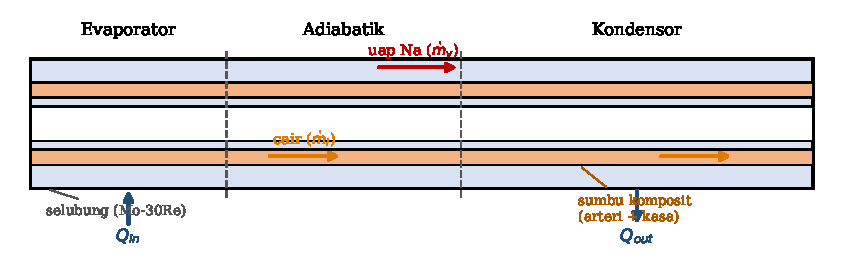
\includegraphics[width=0.9\linewidth,height=\textheight,keepaspectratio]{figures/skema_pipa_kalor.pdf}

}

\caption{\label{fig-skema}Skema pipa kalor natrium in-pin beserta arah
aliran uap dan cairan.}

\end{figure}%

Model dibangun atas lima asumsi yang perlu dinyatakan sejak awal karena
membatasi keberlakuannya.

\begin{enumerate}
\def\labelenumi{\arabic{enumi}.}
\tightlist
\item
  Aliran tunak (\emph{steady state}). Tidak ada suku akumulasi massa,
  momentum, maupun energi.
\item
  Uap berada dalam kesetimbangan saturasi lokal, sehingga
  \(T(z) = T_{sat}(P_v(z))\). Asumsi ini wajar untuk pipa kalor logam
  cair karena laju penguapan dan pengembunan jauh lebih cepat daripada
  transpor aksial.
\item
  Aliran uap satu dimensi aksial, seragam pada setiap penampang, dengan
  faktor gesek Darcy yang bergantung pada bilangan Reynolds lokal.
\item
  Sumbu berpori jenuh sempurna; aliran cairan mengikuti hukum Darcy yang
  diperluas dengan suku inersia Ergun.
\item
  Hambatan termal radial dihitung dengan jaringan satu dimensi,
  sedangkan konduksi aksial pada selubung diabaikan karena rasio panjang
  terhadap tebal dinding sangat besar.
\end{enumerate}

\section{Sifat Termofisika Natrium}\label{sifat-termofisika-natrium}

Sifat natrium cair dan uap dievaluasi dari korelasi Fink dan Leibowitz
{[}12{]} beserta korelasi pelengkap dari Faghri {[}6{]}. Densitas cairan
mengikuti hubungan linear

\begin{equation}\protect\phantomsection\label{eq-rhol}{\rho_l(T) = 1014 - 0{,}235\,T \quad [\mathrm{kg/m^3}]}\end{equation}

yang berlaku dalam 1\% pada rentang 400--1400 K. Viskositas dinamis
cairan dinyatakan sebagai

\begin{equation}\protect\phantomsection\label{eq-mul}{\ln \mu_l = -6{,}4406 - 0{,}3958 \ln T + \frac{556{,}835}{T} \quad [\mathrm{Pa\cdot s}]}\end{equation}

Tegangan permukaan mengikuti bentuk Watson yang dipatri pada temperatur
kritis \(T_c = 2503{,}7\) K,

\begin{equation}\protect\phantomsection\label{eq-sigma}{\sigma(T) = 0{,}2405 \left(1 - \frac{T}{T_c}\right)^{1{,}126} \quad [\mathrm{N/m}]}\end{equation}

dan kalor laten penguapan mengikuti bentuk serupa,

\begin{equation}\protect\phantomsection\label{eq-hfg}{h_{fg}(T) = 4{,}76 \times 10^{6} \left(1 - \frac{T}{T_c}\right)^{0{,}38} \quad [\mathrm{J/kg}]}\end{equation}

Persoalan muncul pada tekanan uap jenuh. Korelasi yang lazim dikutip
untuk natrium ditulis dalam bentuk tertutup dengan konstanta yang
berbeda-beda antar sumber, sehingga pada 1000 K hasilnya dapat berbeda
lebih dari satu orde besaran. Karena tekanan uap menentukan densitas uap
dan melalui densitas itu menentukan batas sonik, kesalahan pada besaran
ini akan merambat ke seluruh kesimpulan desain.

Untuk menghindari inkonsistensi tersebut, penelitian ini tidak memakai
korelasi tertutup, melainkan mengintegrasikan persamaan
Clausius--Clapeyron dengan kalor laten pada (Persamaan~\ref{eq-hfg}),

\begin{equation}\protect\phantomsection\label{eq-clapeyron}{\frac{d \ln P_{sat}}{dT} = \frac{h_{fg}(T)}{R_g T^{2}}}\end{equation}

dari titik didih normal \(T_b = 1156{,}2\) K tempat
\(P_{sat} = 101{,}325\) kPa, dengan \(R_g = R_u/M_{Na} = 361{,}66\)
J/(kg·K). Integrasi numerik dilakukan pada grid 0,25 K menggunakan
aturan trapesium. Cara ini menjamin bahwa kurva tekanan uap dan kurva
kalor laten yang dipakai model saling konsisten secara termodinamika.
Hasilnya adalah \(P_{sat}(1000\ \mathrm{K}) = 24{,}07\) kPa dan
\(P_{sat}(1075\ \mathrm{K}) = 50{,}1\) kPa.

Densitas uap dihitung dengan hukum gas ideal untuk natrium monomer,
\(\rho_v = P_v/(R_g T)\). Koreksi dimerisasi diabaikan; pada 1000--1100
K fraksi dimer natrium masih di bawah 8\%, sehingga kesalahan densitas
yang ditimbulkan tetap lebih kecil daripada ketidakpastian korelasi
tekanan uap itu sendiri.

\begin{figure}[htbp]

\centering{

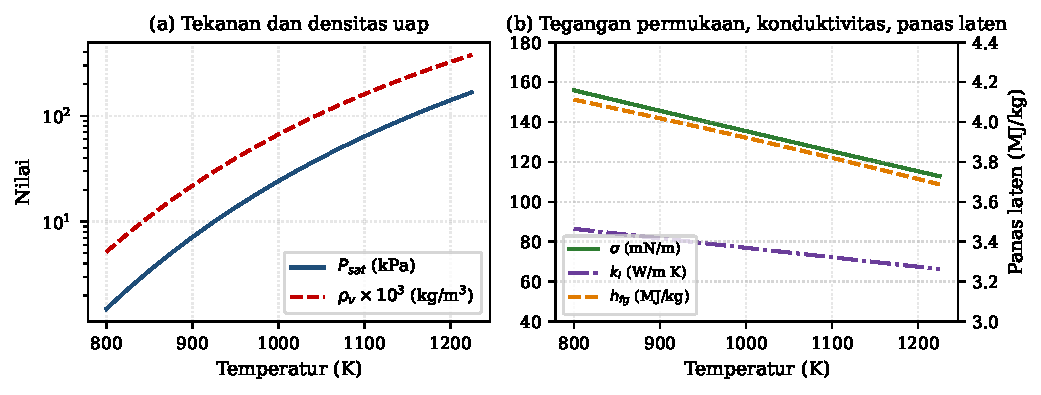
\includegraphics[width=0.95\linewidth,height=\textheight,keepaspectratio]{figures/sifat_natrium.pdf}

}

\caption{\label{fig-sifat}Sifat termofisika natrium jenuh pada rentang
operasi reaktor antariksa: (a) tekanan uap jenuh dan densitas uap; (b)
tegangan permukaan, konduktivitas termal, dan kalor laten.}

\end{figure}%

\begin{longtable}[]{@{}
  >{\centering\arraybackslash}p{(\linewidth - 14\tabcolsep) * \real{0.1250}}
  >{\centering\arraybackslash}p{(\linewidth - 14\tabcolsep) * \real{0.1250}}
  >{\centering\arraybackslash}p{(\linewidth - 14\tabcolsep) * \real{0.1250}}
  >{\centering\arraybackslash}p{(\linewidth - 14\tabcolsep) * \real{0.1250}}
  >{\centering\arraybackslash}p{(\linewidth - 14\tabcolsep) * \real{0.1250}}
  >{\centering\arraybackslash}p{(\linewidth - 14\tabcolsep) * \real{0.1250}}
  >{\centering\arraybackslash}p{(\linewidth - 14\tabcolsep) * \real{0.1250}}
  >{\centering\arraybackslash}p{(\linewidth - 14\tabcolsep) * \real{0.1250}}@{}}
\caption{Sifat termofisika natrium jenuh pada rentang operasi reaktor
antariksa.}\label{tbl-sifat}\tabularnewline
\toprule\noalign{}
\begin{minipage}[b]{\linewidth}\centering
\(T\) (K)
\end{minipage} & \begin{minipage}[b]{\linewidth}\centering
\(P_{sat}\) (kPa)
\end{minipage} & \begin{minipage}[b]{\linewidth}\centering
\(\rho_l\) (kg/m³)
\end{minipage} & \begin{minipage}[b]{\linewidth}\centering
\(\rho_v\) (kg/m³)
\end{minipage} & \begin{minipage}[b]{\linewidth}\centering
\(\mu_l\) (µPa·s)
\end{minipage} & \begin{minipage}[b]{\linewidth}\centering
\(h_{fg}\) (MJ/kg)
\end{minipage} & \begin{minipage}[b]{\linewidth}\centering
\(\sigma\) (mN/m)
\end{minipage} & \begin{minipage}[b]{\linewidth}\centering
\(k_l\) (W/m·K)
\end{minipage} \\
\midrule\noalign{}
\endfirsthead
\toprule\noalign{}
\begin{minipage}[b]{\linewidth}\centering
\(T\) (K)
\end{minipage} & \begin{minipage}[b]{\linewidth}\centering
\(P_{sat}\) (kPa)
\end{minipage} & \begin{minipage}[b]{\linewidth}\centering
\(\rho_l\) (kg/m³)
\end{minipage} & \begin{minipage}[b]{\linewidth}\centering
\(\rho_v\) (kg/m³)
\end{minipage} & \begin{minipage}[b]{\linewidth}\centering
\(\mu_l\) (µPa·s)
\end{minipage} & \begin{minipage}[b]{\linewidth}\centering
\(h_{fg}\) (MJ/kg)
\end{minipage} & \begin{minipage}[b]{\linewidth}\centering
\(\sigma\) (mN/m)
\end{minipage} & \begin{minipage}[b]{\linewidth}\centering
\(k_l\) (W/m·K)
\end{minipage} \\
\midrule\noalign{}
\endhead
\bottomrule\noalign{}
\endlastfoot
800 & 1,49 & 826 & 0,0051 & 227,1 & 4,11 & 155,9 & 86,5 \\
900 & 7,10 & 802 & 0,0218 & 200,6 & 4,02 & 145,6 & 81,8 \\
1.000 & 24,07 & 779 & 0,0666 & 180,8 & 3,92 & 135,5 & 77,0 \\
1.100 & 63,73 & 756 & 0,1602 & 165,6 & 3,82 & 125,4 & 72,2 \\
1.200 & 140,37 & 732 & 0,3234 & 153,3 & 3,71 & 115,3 & 67,5 \\
\end{longtable}

\section{Momentum Uap Kompresibel Satu
Dimensi}\label{momentum-uap-kompresibel-satu-dimensi}

Laju alir massa uap pada setiap posisi aksial ditentukan oleh fluks
penguapan dan pengembunan. Dengan \(Q\) sebagai daya yang ditranspor dan
\(h_{fg}\) dievaluasi pada temperatur kondensor,

\begin{equation}\protect\phantomsection\label{eq-mdot}{\dot m_v(z) = \frac{Q}{h_{fg}} \cdot m(z), \qquad
m(z) = \begin{cases} z/L_e, & 0 \le z \le L_e \\ 1, & L_e < z \le L_e + L_a \\ 1 - (z - L_e - L_a)/L_c, & z > L_e + L_a \end{cases}}\end{equation}

Momentum uap diselesaikan dari persamaan Navier--Stokes satu dimensi
yang dirata-ratakan pada penampang, dengan suku gesekan dinding dan suku
fluks momentum,

\begin{equation}\protect\phantomsection\label{eq-momentum}{\frac{dP_v}{dz} = -\frac{f_v \rho_v u_v^{2}}{2 D_v} - \beta \frac{d(\rho_v u_v^{2})}{dz}}\end{equation}

dengan \(u_v = \dot m_v/(\rho_v A_v)\) dan \(D_v = 2 r_v\). Faktor gesek
Darcy mengikuti rezim aliran,

\begin{equation}\protect\phantomsection\label{eq-fv}{f_v = \begin{cases} 64/Re_v, & Re_v < 2300 \\ 0{,}3164\,Re_v^{-0{,}25}, & Re_v \ge 2300 \end{cases}, \qquad Re_v = \frac{\rho_v u_v D_v}{\mu_v}}\end{equation}

Koefisien \(\beta\) membedakan injeksi massa pada evaporator
(\(\beta = 1\)) dari pengisapan massa pada kondensor
(\(\beta = 0{,}65\)). Perbedaan ini penting: pada evaporator, penambahan
massa radial mempercepat aliran aksial sehingga menambah rugi tekanan,
sedangkan pada kondensor pengisapan memperlambat aliran sehingga terjadi
pemulihan tekanan parsial {[}6{]}.

Karena \(T\) dan \(P\) terikat oleh kesetimbangan saturasi,
(Persamaan~\ref{eq-momentum}) merupakan persamaan diferensial biasa
untuk \(P_v(z)\) saja. Persamaan tersebut diintegrasikan mundur dari
\(z = L\), tempat \(P_v = P_{sat}(T_c)\) dan \(u_v = 0\), menuju
\(z = 0\) dengan metode Runge--Kutta orde empat pada 240 titik grid.
Hasilnya adalah profil tekanan, temperatur, kecepatan, dan bilangan Mach
sepanjang pipa.

Bilangan Mach lokal dihitung dengan kecepatan suara uap monatomik,

\begin{equation}\protect\phantomsection\label{eq-mach}{c_s = \sqrt{\gamma R_g T}, \qquad Ma(z) = \frac{u_v(z)}{c_s}, \qquad \gamma = 5/3}\end{equation}

\section{Aliran Balik Cairan pada Sumbu
Komposit}\label{aliran-balik-cairan-pada-sumbu-komposit}

Cairan yang terkondensasi di kondensor harus kembali ke evaporator
melalui sumbu berpori. Untuk sumbu komposit yang terdiri atas arteri
annular terbuka dan lapisan kasa halus pembentuk meniskus, aliran cairan
mengikuti

\begin{equation}\protect\phantomsection\label{eq-darcy}{\frac{dP_l}{dz} = \frac{\mu_l \dot m_l}{\rho_l A_w K} + \frac{\rho_l g \sin\psi}{1}}\end{equation}

dengan \(A_w\) luas penampang aliran efektif sumbu dan \(K\)
permeabilitas. Suku inersia Ergun diabaikan karena bilangan Reynolds
cairan dalam pori berorde jauh di bawah satu untuk seluruh kasus yang
ditinjau. Kekekalan massa memberikan \(\dot m_l(z) = \dot m_v(z)\),
sehingga profil laju alir cairan identik dengan profil uap.

Nilai permeabilitas ditentukan oleh struktur sumbu. Untuk arteri annular
terbuka dengan celah radial \(b\), pendekatan saluran sempit memberikan
\(K \approx b^{2}/8\); untuk \(b = 0{,}8\) mm diperoleh
\(K \approx 8 \times 10^{-8}\) m\(^{2}\), jauh lebih besar daripada
sumbu kasa tunggal yang hanya berkisar \(10^{-11}\)--\(10^{-10}\)
m\(^{2}\) {[}14{]}. Dalam model ini dipakai nilai konservatif
\(K = 5 \times 10^{-9}\) m\(^{2}\) untuk memperhitungkan penyempitan
akibat dinding arteri dan sisa kasa.

Tekanan kapiler yang tersedia pada meniskus mengikuti persamaan
Young--Laplace,

\begin{equation}\protect\phantomsection\label{eq-laplace}{\Delta P_{c}(z) = P_v(z) - P_l(z) \le \Delta P_{c,maks} = \frac{2\sigma}{r_{eff}}}\end{equation}

dengan \(r_{eff}\) jari-jari pori efektif kasa pembentuk meniskus dan
sudut kontak diambil nol karena natrium membasahi logam refraktori
secara sempurna. Syarat operasi tunak adalah

\begin{equation}\protect\phantomsection\label{eq-neraca-tekanan}{\Delta P_{c,maks} \ge \Delta P_v + \Delta P_l + \Delta P_g}\end{equation}

dengan \(\Delta P_v\) rugi tekanan uap total, \(\Delta P_l\) rugi
tekanan cairan total, dan \(\Delta P_g = \rho_l g L \sin\psi\) komponen
hidrostatik.

\section{Batas-Batas Operasi}\label{batas-batas-operasi}

\subsection{Batas Kapiler}\label{batas-kapiler}

Batas kapiler tercapai ketika kebutuhan tekanan sirkulasi menyamai
tekanan kapiler maksimum. Karena \(\Delta P_v\) tumbuh sebanding
\(Q^{2}\) sedangkan \(\Delta P_l\) sebanding \(Q\), batas ini ditentukan
dengan metode bagi dua (\emph{bisection}) pada \(Q\) hingga
(Persamaan~\ref{eq-neraca-tekanan}) terpenuhi sebagai persamaan.
Pendekatan ini lebih akurat daripada rumus tertutup
\(Q_{cap} = (\Delta P_{c,maks} - \Delta P_g)/[(F_l + F_v)L_{eff}]\) yang
mengabaikan ketergantungan \(F_v\) pada \(Q\).

\subsection{Batas Sonik}\label{batas-sonik}

Ketika temperatur rendah, densitas uap sangat kecil sehingga kecepatan
uap di ujung evaporator dapat mencapai kecepatan suara. Korelasi
Levy--Busse memberikan

\begin{equation}\protect\phantomsection\label{eq-sonic}{Q_{sonic} = A_v \rho_v h_{fg} \sqrt{\frac{\gamma R_g T}{2(\gamma + 1)}}}\end{equation}

Korelasi ini mengasumsikan densitas uap konstan sepanjang pipa. Model
ini juga menghitung bilangan Mach secara langsung dari
(Persamaan~\ref{eq-mach}), sehingga dapat diperiksa apakah korelasi
tersebut konservatif atau tidak.

\subsection{Batas Entrainment}\label{batas-entrainment}

Tetesan cairan terlepas dari permukaan meniskus ketika gaya geser uap
melampaui gaya tegangan permukaan. Kriteria Weber
\(We = \rho_v u_v^{2}(2 r_{eff})/\sigma \ge 1\) memberikan

\begin{equation}\protect\phantomsection\label{eq-ent}{Q_{ent} = A_v h_{fg} \sqrt{\frac{\sigma \rho_v}{2 r_{eff}}}}\end{equation}

\subsection{Batas Viskos}\label{batas-viskos}

Pada temperatur sangat rendah, gradien tekanan viskos dapat mencekik
aliran sebelum rezim sonik tercapai. Batas Busse untuk kasus ini adalah

\begin{equation}\protect\phantomsection\label{eq-visc}{Q_{visc} = \frac{r_v^{2} h_{fg} \rho_v P_{sat} A_v}{16 \mu_v L_{eff}}}\end{equation}

\subsection{Batas Pendidihan}\label{batas-pendidihan}

Jika fluks kalor radial terlalu tinggi, gelembung uap dapat terbentuk di
dalam pori dan mengisolasi dinding dari pasokan cairan. Ambang
terjadinya nukleasi pada rongga berjari-jari \(r_n\) adalah

\begin{equation}\protect\phantomsection\label{eq-boil}{\Delta T_{krit} = \frac{2 \sigma T_{sat}}{\rho_v h_{fg} r_n}, \qquad
Q_{boil} = \frac{2 \pi L_e k_{eff} \Delta T_{krit}}{\ln(r_i/r_v)}}\end{equation}

dengan \(k_{eff}\) konduktivitas efektif sumbu jenuh menurut model
Maxwell--Eucken dan \(r_n = 2{,}5\) µm.

Amplop operasi adalah nilai minimum dari kelima batas,

\begin{equation}\protect\phantomsection\label{eq-env}{Q_{env}(T) = \min\left(Q_{cap},\, Q_{sonic},\, Q_{ent},\, Q_{visc},\, Q_{boil}\right)}\end{equation}

\section{Jaringan Hambatan Termal
Radial}\label{jaringan-hambatan-termal-radial}

Beda temperatur antara dinding evaporator dan dinding kondensor terdiri
atas empat komponen: konduksi radial pada dinding evaporator, konduksi
radial pada sumbu, penurunan temperatur uap akibat gradien tekanan, dan
konduksi radial pada dinding kondensor. Masing-masing dinyatakan sebagai

\begin{equation}\protect\phantomsection\label{eq-rth}{R_{wall} = \frac{\ln(r_o/r_i)}{2\pi k_w L_e}, \quad
R_{wick} = \frac{\ln(r_i/r_v)}{2\pi k_{eff} L_e}, \quad
R_{vap} = \frac{8 \mu_v T}{\pi \rho_v^{2} h_{fg}^{2} r_v^{4}}}\end{equation}

Hambatan total pipa adalah
\(R_{th} = R_{wall} + R_{wick} + R_{cond,wall} + R_{vap}\), dan beda
temperatur totalnya \(\Delta T_{hp} = Q R_{th}\) ditambah penurunan
temperatur saturasi sepanjang inti uap.

\section{Konduksi Radial Pelet Uranium
Nitrida}\label{konduksi-radial-pelet-uranium-nitrida}

Pelet bahan bakar ISR berbentuk anular: panas dibangkitkan di dalam
annulus dan mengalir ke dalam menuju pipa kalor, sedangkan permukaan
luar pelet bersentuhan dengan kelongsong yang secara termal mendekati
adiabatik. Untuk pembangkitan volumetrik seragam \(q'''\) dan temperatur
permukaan dalam \(T_i\), solusi tunak persamaan konduksi satu dimensi
adalah

\begin{equation}\protect\phantomsection\label{eq-fuel}{T(r) = T_i + \frac{q'''}{2k}\left[r_o^{2}\ln\frac{r}{r_i} - \frac{r^{2} - r_i^{2}}{2}\right]}\end{equation}

sehingga kenaikan temperatur puncak di permukaan luar pelet, tempat
\(T\) maksimum, adalah

\begin{equation}\protect\phantomsection\label{eq-dtfuel}{\Delta T_{UN} = \frac{q'''}{2k_{UN}}\left[r_o^{2}\ln\frac{r_o}{r_i} - \frac{r_o^{2} - r_i^{2}}{2}\right]}\end{equation}

dengan \(q''' = Q_{pin}/[\pi(r_o^{2} - r_i^{2})H]\). Persamaan ini
mengabaikan ketergantungan \(k_{UN}\) pada temperatur dan gradasi
pembangkitan akibat \emph{burnup}; keduanya bersifat konservatif karena
menaikkan perkiraan temperatur puncak.

\section{Pengaruh Gravitasi dan Rezim
Mikrogravitasi}\label{pengaruh-gravitasi-dan-rezim-mikrogravitasi}

Komponen hidrostatik \(\Delta P_g = \rho_l g L \sin\psi\) hilang pada
\(g = 0\). Pada pengujian darat dengan evaporator di atas
(\(\psi = 90^\circ\)), suku ini mencapai sekitar 3,4 kPa untuk pipa
sepanjang 0,46 m pada 1075 K, yaitu sekitar 20\% dari tekanan kapiler
maksimum. Karena itu pengujian darat selalu memberikan batas operasi
yang lebih rendah daripada operasi sesungguhnya di orbit, dan perbedaan
tersebut harus diperhitungkan ketika hasil uji bumi dipakai untuk
merancang pipa kalor antariksa.

\section{Hipotesis}\label{hipotesis}

Berdasarkan tinjauan teoretis di atas, diajukan tiga hipotesis.

\begin{enumerate}
\def\labelenumi{\arabic{enumi}.}
\tightlist
\item
  Model tereduksi satu dimensi yang menggabungkan momentum uap
  kompresibel, filtrasi Darcy, dan jaringan hambatan termal mampu
  mereproduksi karakteristik beda temperatur pipa kalor KRUSTY dengan
  kesalahan rata-rata di bawah 10\% pada pengujian \emph{leave-one-out}.
\item
  Pada rentang temperatur kerja 1000--1150 K, mekanisme pembatas pipa
  kalor berukuran diameter luar 16--20 mm adalah batas entrainment,
  bukan batas kapiler sebagaimana lazim diasumsikan pada literatur pipa
  kalor logam cair.
\item
  Penggantian loop pompa Na-78K oleh pipa kalor natrium pada teras ISR
  500 kWth menghasilkan margin keselamatan positif untuk seluruh 61 pin,
  tetapi menuntut pengurangan volume bahan bakar lebih dari 20\% akibat
  pelebaran rongga tengah pin.
\end{enumerate}

\chapter{PELAKSANAAN PENELITIAN}\label{pelaksanaan-penelitian}

\section{Alat dan Bahan Penelitian}\label{alat-dan-bahan-penelitian}

\subsection{Perangkat Lunak}\label{perangkat-lunak}

Seluruh perhitungan dilaksanakan dengan Python 3.12 menggunakan NumPy
untuk operasi larik dan Matplotlib untuk pembuatan gambar. Kode ditulis
sebagai satu paket kecil yang terdiri atas modul sifat termofisika,
modul geometri, penyelesai aksial, modul batas operasi, modul termal
bahan bakar, dan skrip studi yang menghasilkan seluruh tabel dan gambar
pada Bab V. Pendekatan ini dipilih agar setiap angka dalam skripsi dapat
dilacak kembali ke satu baris kode.

Waktu eksekusi satu kali penyelesaian aksial pada grid 240 titik adalah
sekitar 4 ms pada komputer jinjing biasa, sedangkan satu studi lengkap
meliputi pemetaan amplop 12 temperatur, sapuan geometri 8 diameter, dan
5 cincin teras selesai dalam kurang dari satu menit. Kecepatan inilah
yang membedakan model tereduksi dari kode CFD dan yang membuat iterasi
desain menjadi praktis.

\subsection{Bahan dan Data Penelitian}\label{bahan-dan-data-penelitian}

Data yang dipakai terdiri atas tiga kelompok. Kelompok pertama adalah
sifat termofisika natrium dari korelasi Fink dan Leibowitz {[}12{]}.
Kelompok kedua adalah data uji KRUSTY berupa lima kondisi tunak pada
rentang daya 312,5--1000 W per pipa dengan temperatur evaporator
991--1141 K dan beda temperatur terukur 26--56 K {[}8{]}. Kelompok
ketiga adalah parameter desain teras ISR: 61 pin, diameter pelet 32,65
mm, rongga tengah 7,65 mm, tinggi aktif 250 mm, bahan bakar UN dengan
densitas 95\% teoritis, kelongsong Mo-30Re, dan daya total 500 kWth
{[}11{]}.

Data KRUSTY dipakai dalam bentuk beda temperatur antara termokopel
evaporator dan kondensor, bukan temperatur absolut, karena besaran
itulah yang dapat dibandingkan langsung dengan model tanpa memerlukan
informasi mengenai rugi kalor blok pemanas.

\subsection{Parameter Desain Acuan}\label{parameter-desain-acuan}

Parameter geometri dan operasi pipa kalor yang dievaluasi ditampilkan
pada Tabel 4.1. Nilai-nilai tersebut merupakan hasil studi sapuan yang
dibahas pada Bab V; pada tahap pelaksanaan, nilai inilah yang dipakai
sebagai titik desain.

\begin{longtable}[]{@{}lcc@{}}
\caption{Parameter geometri dan operasi pipa kalor acuan untuk teras
ISR.}\label{tbl-parameter}\tabularnewline
\toprule\noalign{}
Parameter & Nilai & Satuan \\
\midrule\noalign{}
\endfirsthead
\toprule\noalign{}
Parameter & Nilai & Satuan \\
\midrule\noalign{}
\endhead
\bottomrule\noalign{}
\endlastfoot
Diameter luar selubung \(D_o\) & 18,0 & mm \\
Tebal dinding Mo-30Re & 0,9 & mm \\
Tebal sumbu komposit & 0,8 & mm \\
Diameter inti uap \(D_v\) & 14,6 & mm \\
Jari-jari pori efektif \(r_{eff}\) & 15 & µm \\
Permeabilitas sumbu \(K\) & \(5\times10^{-9}\) & m² \\
Panjang evaporator \(L_e\) & 250 & mm \\
Panjang adiabatik \(L_a\) & 50 & mm \\
Panjang kondensor \(L_c\) & 160 & mm \\
Temperatur uap evaporator & 1075 & K \\
Fluida kerja & Natrium & -- \\
Daya pin rata-rata & 8,20 & kWth \\
Daya pin puncak (\(F_r\) = 1,35) & 11,07 & kWth \\
\end{longtable}

\section{Tata Laksana Penelitian}\label{tata-laksana-penelitian}

Penelitian dilaksanakan dalam enam tahap yang saling bergantung (Gambar
4.1). Tahap pertama adalah konsolidasi literatur dan data sekunder, yang
menghasilkan himpunan korelasi sifat, geometri acuan, dan data validasi.
Tahap kedua adalah formulasi dan implementasi model. Tahap ketiga adalah
verifikasi numerik, yaitu pemeriksaan bahwa kode menyelesaikan persamaan
yang dimaksud dan bahwa hasilnya tidak bergantung pada grid. Tahap
keempat adalah validasi terhadap data KRUSTY. Tahap kelima adalah
penerapan pada teras ISR, meliputi pemetaan amplop, optimasi geometri,
integrasi teras, dan analisis kegagalan. Tahap keenam adalah analisis
massa, daya parasitik, dan perumusan kesimpulan.

\begin{figure}[htbp]

\centering{

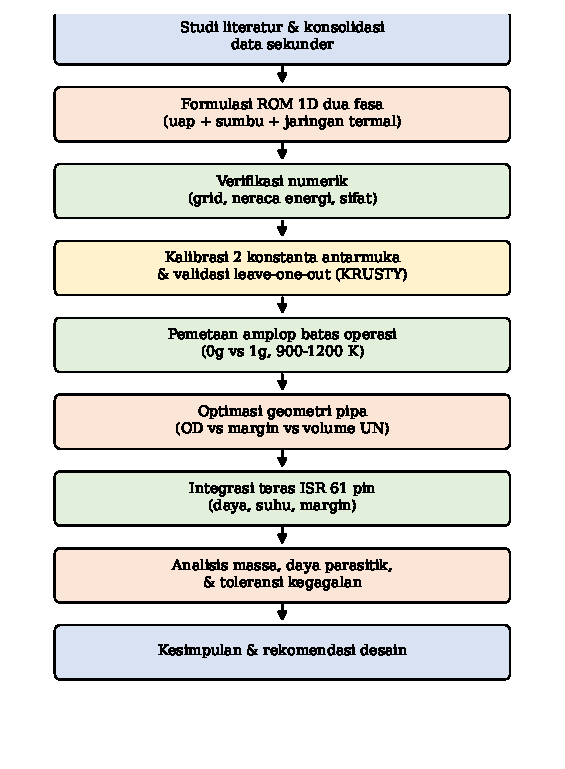
\includegraphics[width=0.55\linewidth,height=\textheight,keepaspectratio]{figures/diagram_alir.pdf}

}

\caption{\label{fig-alir}Diagram alir pelaksanaan penelitian.}

\end{figure}%

\subsection{Algoritma Penyelesaian}\label{algoritma-penyelesaian}

Penyelesaian aksial berjalan sebagai berikut.

\begin{enumerate}
\def\labelenumi{\arabic{enumi}.}
\tightlist
\item
  Tetapkan daya \(Q\), temperatur kondensor \(T_c\), geometri, dan
  kondisi gravitasi.
\item
  Hitung \(\dot m_{maks} = Q/h_{fg}(T_c)\) dan bentuk profil \(m(z)\)
  menurut (Persamaan~\ref{eq-mdot}).
\item
  Tetapkan \(P_v(L) = P_{sat}(T_c)\) dan \(u_v(L) = 0\) sebagai syarat
  batas di ujung kondensor.
\item
  Integrasikan (Persamaan~\ref{eq-momentum}) mundur dari \(z = L\)
  menuju \(z = 0\) dengan Runge--Kutta orde empat. Pada setiap langkah,
  temperatur diambil dari \(T_{sat}(P_v)\), densitas dari hukum gas
  ideal, dan faktor gesek dari bilangan Reynolds lokal.
\item
  Integrasikan (Persamaan~\ref{eq-darcy}) mundur untuk memperoleh
  \(P_l(z)\), lalu hitung \(\Delta P_c(z) = P_v - P_l\) dan jari-jari
  meniskus lokal \(r_c = 2\sigma/\Delta P_c\).
\item
  Hitung \(\Delta P_{req} = \Delta P_v + \Delta P_l + \Delta P_g\) dan
  bandingkan dengan \(\Delta P_{c,maks}\).
\item
  Untuk batas kapiler, ulangi langkah 1--6 dengan metode bagi dua pada
  \(Q\) hingga \(\Delta P_{req} = \Delta P_{c,maks}\).
\end{enumerate}

Langkah 7 membutuhkan sekitar 40 iterasi bagi dua, masing-masing dengan
satu penyelesaian aksial pada grid kasar 80 titik. Strategi dua grid ini
dipakai untuk menjaga waktu komputasi tetap rendah tanpa mengorbankan
akurasi, karena batas kapiler hanya bergantung pada nilai integral
tekanan.

\subsection{Verifikasi Numerik}\label{verifikasi-numerik}

Verifikasi dilakukan melalui lima uji yang masing-masing memeriksa satu
aspek berbeda.

\begin{enumerate}
\def\labelenumi{\arabic{enumi}.}
\tightlist
\item
  \textbf{Konvergensi grid.} Penyelesaian diulang pada \(N\) = 30, 60,
  120, 240, dan 480 titik, lalu deviasi relatif \(\Delta P_v\) terhadap
  solusi \(N\) = 1920 dihitung.
\item
  \textbf{Neraca energi.} Diperiksa bahwa \(\dot m_{maks} h_{fg}\) tepat
  sama dengan \(Q\) yang ditetapkan.
\item
  \textbf{Aliran cairan.} Rugi tekanan cairan hasil integrasi numerik
  dibandingkan dengan solusi Darcy analitik \(Q F_l L_{eff}\).
\item
  \textbf{Aliran uap.} Rugi tekanan uap pada kasus bermassa konstan
  dibandingkan dengan solusi Hagen--Poiseuille.
\item
  \textbf{Jangkar sifat.} Nilai \(T_b\), \(\rho_l(1000\ \mathrm{K})\),
  \(\sigma(1000\ \mathrm{K})\), \(h_{fg}(1000\ \mathrm{K})\), dan
  \(P_{sat}(1000\ \mathrm{K})\) dibandingkan dengan nilai rujukan.
\end{enumerate}

\subsection{Protokol Validasi}\label{protokol-validasi}

Validasi terhadap data KRUSTY tidak dilakukan dengan menyesuaikan model
agar cocok, melainkan dengan memisahkan parameter kalibrasi dari
parameter uji. Beda temperatur terukur mengandung dua kontribusi: beda
temperatur intrinsik pipa, yang dihitung model, dan beda temperatur
antarmuka antara blok pemanas, dinding evaporator, klem kondensor, dan
kalorimeter, yang tidak dimodelkan. Kontribusi kedua didekati dengan
bentuk linear

\begin{equation}\protect\phantomsection\label{eq-kalibrasi}{\Delta T_{pred}(Q) = \Delta T_{hp}(Q) + R_{int} Q + b}\end{equation}

dengan \(R_{int}\) hambatan antarmuka dan \(b\) offset instrumental.
Kedua konstanta ditentukan dengan kuadrat terkecil pada empat titik,
lalu dipakai untuk memprediksi titik kelima; prosedur ini diulang lima
kali sehingga setiap titik pernah menjadi titik uji
(\emph{leave-one-out}).

Nilai \(R_{int}\) yang diperoleh kemudian diperiksa kewajarannya secara
independen. Konduktansi kontak antara dua permukaan logam yang diklem
biasanya berkisar 1000--3000 W/(m²·K); dengan luas kontak efektif 0,015
m², hambatan yang dihasilkan adalah 0,022--0,067 K/W. Apabila nilai
kalibrasi jatuh di dalam rentang tersebut, maka parameter kalibrasi
memiliki dasar fisik dan bukan sekadar pemasangan kurva.

\subsection{Metrik Evaluasi}\label{metrik-evaluasi}

Akurasi validasi dinyatakan dengan \emph{mean absolute percentage error}
(MAPE), \emph{root mean square error} (RMSE), dan koefisien determinasi
\(R^{2}\),

\begin{equation}\protect\phantomsection\label{eq-metrik}{\mathrm{MAPE} = \frac{100\%}{n}\sum_{i=1}^{n}\left|\frac{y_i - \hat y_i}{y_i}\right|, \qquad
R^{2} = 1 - \frac{\sum (y_i - \hat y_i)^{2}}{\sum (y_i - \bar y)^{2}}}\end{equation}

Kinerja teras dinyatakan dengan faktor keselamatan
\(SF = Q_{env}/Q_{pin}\) dan margin tekanan kapiler

\begin{equation}\protect\phantomsection\label{eq-margin}{M = \frac{\Delta P_{c,maks} - \Delta P_{req}}{\Delta P_{c,maks}} \times 100\%}\end{equation}

Kriteria keberterimaan yang dipakai adalah \(SF \ge 1{,}3\) pada pin
puncak, \(M > 0\) untuk seluruh pin, dan temperatur puncak bahan bakar
di bawah 1650 K. Batas 1650 K dipilih lebih konservatif daripada titik
leleh UN (3073 K) karena uranium nitrida mengalami disosiasi signifikan
di atas 1900 K dalam lingkungan vakum, sehingga integritas bahan bakar
lebih baik dijaga dengan margin yang lebar.

\section{Rencana Analisis Hasil}\label{rencana-analisis-hasil}

Analisis hasil dibagi menjadi enam bagian yang masing-masing menjawab
satu pertanyaan penelitian. Bagian pertama menyajikan verifikasi dan
validasi, termasuk pembahasan mengapa sebagian deviasi tidak dapat
dihilangkan oleh model satu dimensi. Bagian kedua memetakan amplop
operasi pada kondisi mikrogravitasi dan membandingkannya dengan kondisi
pengujian darat. Bagian ketiga membahas profil aksial pada titik beban
puncak, terutama perilaku tekanan kapiler dan bilangan Mach. Bagian
keempat menyajikan optimasi geometri, dengan kriteria pemilihan yang
dinyatakan eksplisit. Bagian kelima mengintegrasikan hasil ke seluruh 61
pin teras, termasuk evaluasi kegagalan satu dan dua pipa. Bagian keenam
menutup dengan neraca massa, daya parasitik, dan pembahasan
keterbatasan.

\chapter{HASIL DAN PEMBAHASAN}\label{hasil-dan-pembahasan}

\section{Verifikasi Numerik}\label{verifikasi-numerik-1}

Sebelum model dipakai untuk mengambil keputusan desain, harus dipastikan
lebih dahulu bahwa kode menyelesaikan persamaan yang dimaksud. Tabel 5.1
merangkum lima uji verifikasi yang dijalankan.

\begin{longtable}[]{@{}llccc@{}}
\caption{Hasil verifikasi numerik dan konsistensi
model.}\label{tbl-verifikasi}\tabularnewline
\toprule\noalign{}
Uji & Parameter & Model & Acuan & Dev. (\%) \\
\midrule\noalign{}
\endfirsthead
\toprule\noalign{}
Uji & Parameter & Model & Acuan & Dev. (\%) \\
\midrule\noalign{}
\endhead
\bottomrule\noalign{}
\endlastfoot
Grid & N=30 & 512,89 & 514,31 & 0,28 \\
Grid & N=60 & 514,09 & 514,31 & 0,04 \\
Grid & N=120 & 514,18 & 514,31 & 0,03 \\
Grid & N=240 & 514,33 & 514,31 & 0,00 \\
Grid & N=480 & 514,37 & 514,31 & 0,01 \\
Energi & \(\dot m h_{fg}\) vs \(Q\) & 11.072,66 & 11.072,66 & 0,00 \\
Cairan & vs Darcy & 2.106,14 & 2.105,67 & 0,02 \\
Uap & vs Hagen-Poiseuille & 0,7816 & 0,7835 & 0,25 \\
Sifat & \(T_{didih}\) (K) & 1.156,25 & 1.156,20 & 0,00 \\
Sifat & \(\rho_l\) 1000 K (kg/m³) & 779,00 & 780,00 & 0,13 \\
Sifat & \(\sigma\) 1000 K (N/m) & 0,1355 & 0,1350 & 0,34 \\
Sifat & \(h_{fg}\) 1000 K (MJ/kg) & 3,9216 & 3,9000 & 0,55 \\
Sifat & \(P_{sat}\) 1000 K (kPa) & 24,0741 & 24,0000 & 0,31 \\
\end{longtable}

Uji konvergensi grid menunjukkan bahwa rugi tekanan uap sudah stabil
pada grid kasar: dengan 30 titik, deviasi terhadap solusi acuan 1920
titik hanya 0,28\%, dan pada 120 titik deviasi turun menjadi 0,03\%.
Pola ini khas untuk integrasi Runge--Kutta orde empat pada persamaan
yang halus, dan menjadi alasan mengapa grid 240 titik dipakai pada
seluruh perhitungan berikutnya: akurasi yang diperoleh sudah jauh
melampaui ketidakpastian korelasi sifat termofisika.

Neraca energi terpenuhi secara eksak karena laju alir massa ditetapkan
dari daya dan kalor laten. Uji yang lebih bermakna adalah perbandingan
komponen rugi tekanan dengan solusi analitik. Rugi tekanan cairan hasil
integrasi numerik berbeda 0,02\% dari solusi Darcy analitik, sedangkan
rugi tekanan uap pada kasus bermassa konstan berbeda 0,25\% dari solusi
Hagen--Poiseuille. Kedua angka ini menunjukkan bahwa skema integrasi dan
penanganan syarat batas bekerja sebagaimana mestinya, bukan sekadar
menghasilkan angka yang masuk akal.

Uji jangkar sifat mengonfirmasi bahwa kelima korelasi yang dipakai
konsisten dengan nilai rujukan pada 1000 K, dengan deviasi terbesar
0,55\% pada kalor laten. Yang paling penting adalah titik didih:
integrasi Clausius--Clapeyron mengembalikan 1156,25 K, berbeda 0,004\%
dari nilai 1156,2 K yang menjadi jangkar integrasi, sehingga tidak ada
galat akumulasi yang berarti.

Sebagai pemeriksaan tambahan, bilangan Mach maksimum pada titik beban
puncak adalah 0,165. Nilai ini jauh di bawah satu, sehingga aliran uap
pada titik desain berada pada rezim subsonik dan korelasi batas sonik
tidak perlu dipakai secara langsung untuk menilai kelayakan; korelasi
tersebut tetap dihitung sebagai pembanding pada pemetaan amplop.

\section{Validasi terhadap Uji
KRUSTY}\label{validasi-terhadap-uji-krusty}

Validasi dilakukan terhadap lima kondisi tunak uji KRUSTY pada rentang
312,5--1000 W per pipa. Model menghitung beda temperatur intrinsik pipa
\(\Delta T_{hp}\) terlebih dahulu, kemudian dua konstanta antarmuka
dikalibrasi dengan skema \emph{leave-one-out}.

\begin{longtable}[]{@{}
  >{\centering\arraybackslash}p{(\linewidth - 14\tabcolsep) * \real{0.1250}}
  >{\centering\arraybackslash}p{(\linewidth - 14\tabcolsep) * \real{0.1250}}
  >{\centering\arraybackslash}p{(\linewidth - 14\tabcolsep) * \real{0.1250}}
  >{\centering\arraybackslash}p{(\linewidth - 14\tabcolsep) * \real{0.1250}}
  >{\centering\arraybackslash}p{(\linewidth - 14\tabcolsep) * \real{0.1250}}
  >{\centering\arraybackslash}p{(\linewidth - 14\tabcolsep) * \real{0.1250}}
  >{\centering\arraybackslash}p{(\linewidth - 14\tabcolsep) * \real{0.1250}}
  >{\centering\arraybackslash}p{(\linewidth - 14\tabcolsep) * \real{0.1250}}@{}}
\caption{Perbandingan prediksi model dengan data uji KRUSTY;
\(\Delta T_{hp}\) adalah beda suhu intrinsik pipa dan
\(\Delta T_{pred}\) adalah prediksi
\emph{leave-one-out}.}\label{tbl-krusty}\tabularnewline
\toprule\noalign{}
\begin{minipage}[b]{\linewidth}\centering
Titik uji
\end{minipage} & \begin{minipage}[b]{\linewidth}\centering
\(Q\) (W)
\end{minipage} & \begin{minipage}[b]{\linewidth}\centering
\(T_{e,exp}\) (K)
\end{minipage} & \begin{minipage}[b]{\linewidth}\centering
\(T_{c,exp}\) (K)
\end{minipage} & \begin{minipage}[b]{\linewidth}\centering
\(\Delta T_{exp}\) (K)
\end{minipage} & \begin{minipage}[b]{\linewidth}\centering
\(\Delta T_{hp}\) (K)
\end{minipage} & \begin{minipage}[b]{\linewidth}\centering
\(\Delta T_{pred}\) (K)
\end{minipage} & \begin{minipage}[b]{\linewidth}\centering
Galat LOO (\%)
\end{minipage} \\
\midrule\noalign{}
\endfirsthead
\toprule\noalign{}
\begin{minipage}[b]{\linewidth}\centering
Titik uji
\end{minipage} & \begin{minipage}[b]{\linewidth}\centering
\(Q\) (W)
\end{minipage} & \begin{minipage}[b]{\linewidth}\centering
\(T_{e,exp}\) (K)
\end{minipage} & \begin{minipage}[b]{\linewidth}\centering
\(T_{c,exp}\) (K)
\end{minipage} & \begin{minipage}[b]{\linewidth}\centering
\(\Delta T_{exp}\) (K)
\end{minipage} & \begin{minipage}[b]{\linewidth}\centering
\(\Delta T_{hp}\) (K)
\end{minipage} & \begin{minipage}[b]{\linewidth}\centering
\(\Delta T_{pred}\) (K)
\end{minipage} & \begin{minipage}[b]{\linewidth}\centering
Galat LOO (\%)
\end{minipage} \\
\midrule\noalign{}
\endhead
\bottomrule\noalign{}
\endlastfoot
KRUSTY-SS-1 & 312,5 & 991,15 & 965,15 & 26,0 & 1,55 & 24,71 & 4,96 \\
KRUSTY-SS-2 & 450,0 & 1.025,15 & 993,15 & 32,0 & 2,10 & 30,91 & 3,42 \\
KRUSTY-SS-3 & 625,0 & 1.068,15 & 1.031,15 & 37,0 & 2,79 & 39,09 &
5,66 \\
KRUSTY-SS-4 & 820,0 & 1.107,15 & 1.061,15 & 46,0 & 3,61 & 47,41 &
3,07 \\
KRUSTY-SS-5 & 1.000,0 & 1.141,15 & 1.085,15 & 56,0 & 4,37 & 52,48 &
6,29 \\
\end{longtable}

Hasil kalibrasi memberikan \(R_{int} = 0{,}0384\) K/W dan
\(b = 11{,}86\) K. Nilai \(R_{int}\) berada di dalam rentang
0,022--0,067 K/W yang diperkirakan secara independen dari konduktansi
kontak logam, sehingga parameter kalibrasi ini memiliki dasar fisik dan
bukan sekadar pemasangan kurva. Offset \(b\) sebesar 11,86 K
mencerminkan bahwa termokopel kondensor tidak berada tepat pada
antarmuka uap-kondensat, sehingga selalu membaca temperatur yang lebih
rendah daripada temperatur saturasi di dalam pipa.

Dengan protokol tersebut, diperoleh MAPE 4,68\%, RMSE 2,08 K, dan
\(R^{2} = 0{,}961\); galat terbesar 6,29\% terjadi pada titik daya
tertinggi (\(Q\) = 1000 W). Nilai ini menunjukkan bahwa model mampu
memprediksi beda temperatur pada titik yang tidak dipakai untuk
kalibrasi dalam batas sekitar 5\%, yang untuk keperluan penyaringan
geometri lebih dari memadai.

\begin{figure}[htbp]

\centering{

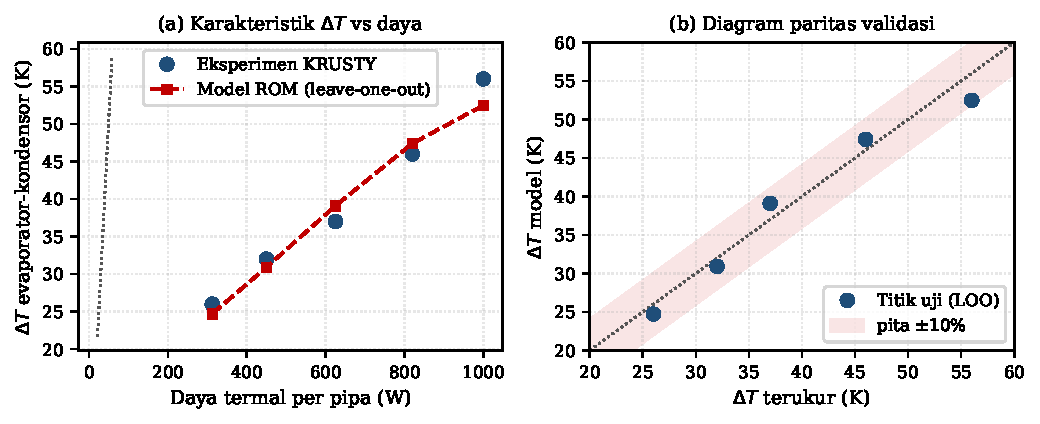
\includegraphics[width=0.95\linewidth,height=\textheight,keepaspectratio]{figures/validasi_profil.pdf}

}

\caption{\label{fig-validasi}(a) Karakteristik beda temperatur terhadap
daya: data uji KRUSTY dan prediksi model \emph{leave-one-out}; (b)
diagram paritas dengan pita \(\pm10\%\).}

\end{figure}%

Yang perlu ditekankan adalah besarnya \(\Delta T_{hp}\) itu sendiri:
hanya 1,55 K pada 312,5 W dan 4,37 K pada 1000 W, sehingga hambatan
termal intrinsik pipa berada pada 4,4--5,0\(\times10^{-3}\) K/W. Angka
ini sesuai dengan hambatan termal pipa kalor natrium yang dilaporkan
pada literatur, yaitu orde \(10^{-3}\) K/W untuk pipa sepanjang satu
meter dengan inti uap belasan milimeter {[}6, 10{]}. Dengan kata lain,
hampir seluruh beda temperatur yang terukur pada uji KRUSTY berasal dari
antarmuka pengujian, bukan dari pipanya. Model satu dimensi karena itu
tidak dapat dan tidak seharusnya dipaksa mencocokkan beda temperatur
total tanpa parameter antarmuka.

Konsekuensi metodologisnya penting bagi Bab V selanjutnya: ketika model
diterapkan pada teras ISR, yang dilaporkan adalah temperatur dinding dan
temperatur bahan bakar yang dihitung dari fisika pipa, bukan temperatur
yang dipengaruhi kondisi pengujian. Ketidakpastian yang tersisa adalah
ketidakpastian model fisika, bukan ketidakpastian antarmuka.

\section{Karakteristik Amplop Operasi dan Pengaruh
Mikrogravitasi}\label{karakteristik-amplop-operasi-dan-pengaruh-mikrogravitasi}

Pemetaan amplop operasi dilakukan pada rentang 900--1150 K, yaitu
rentang yang mencakup seluruh kemungkinan titik kerja teras ISR. Tabel
5.3 menyajikan nilai kelima batas pada beberapa temperatur kunci,
sedangkan Gambar 5.2 menampilkannya secara kontinu.

\begin{longtable}[]{@{}
  >{\centering\arraybackslash}p{(\linewidth - 12\tabcolsep) * \real{0.1429}}
  >{\centering\arraybackslash}p{(\linewidth - 12\tabcolsep) * \real{0.1429}}
  >{\centering\arraybackslash}p{(\linewidth - 12\tabcolsep) * \real{0.1429}}
  >{\centering\arraybackslash}p{(\linewidth - 12\tabcolsep) * \real{0.1429}}
  >{\centering\arraybackslash}p{(\linewidth - 12\tabcolsep) * \real{0.1429}}
  >{\centering\arraybackslash}p{(\linewidth - 12\tabcolsep) * \real{0.1429}}
  >{\centering\arraybackslash}p{(\linewidth - 12\tabcolsep) * \real{0.1429}}@{}}
\caption{Batas-batas perpindahan kalor pipa acuan (OD 18 mm) pada
kondisi mikrogravitasi.}\label{tbl-amplop}\tabularnewline
\toprule\noalign{}
\begin{minipage}[b]{\linewidth}\centering
\(T\) (K)
\end{minipage} & \begin{minipage}[b]{\linewidth}\centering
\(Q_{cap}\) (kW)
\end{minipage} & \begin{minipage}[b]{\linewidth}\centering
\(Q_{sonic}\) (kW)
\end{minipage} & \begin{minipage}[b]{\linewidth}\centering
\(Q_{ent}\) (kW)
\end{minipage} & \begin{minipage}[b]{\linewidth}\centering
\(Q_{boil}\) (kW)
\end{minipage} & \begin{minipage}[b]{\linewidth}\centering
\(Q_{visc}\) (kW)
\end{minipage} & \begin{minipage}[b]{\linewidth}\centering
Pembatas
\end{minipage} \\
\midrule\noalign{}
\endfirsthead
\toprule\noalign{}
\begin{minipage}[b]{\linewidth}\centering
\(T\) (K)
\end{minipage} & \begin{minipage}[b]{\linewidth}\centering
\(Q_{cap}\) (kW)
\end{minipage} & \begin{minipage}[b]{\linewidth}\centering
\(Q_{sonic}\) (kW)
\end{minipage} & \begin{minipage}[b]{\linewidth}\centering
\(Q_{ent}\) (kW)
\end{minipage} & \begin{minipage}[b]{\linewidth}\centering
\(Q_{boil}\) (kW)
\end{minipage} & \begin{minipage}[b]{\linewidth}\centering
\(Q_{visc}\) (kW)
\end{minipage} & \begin{minipage}[b]{\linewidth}\centering
Pembatas
\end{minipage} \\
\midrule\noalign{}
\endhead
\bottomrule\noalign{}
\endlastfoot
900 & 35,63 & 4,68 & 6,93 & 1.000,4 & 49,1 & Sonik \\
950 & 39,71 & 8,59 & 9,04 & 559,2 & 162,9 & Sonik \\
1.000 & 44,62 & 14,69 & 11,38 & 333,5 & 469,9 & Entrainment \\
1.050 & 49,65 & 23,65 & 13,91 & 210,1 & 1.203,1 & Entrainment \\
1.075 & 51,97 & 29,41 & 15,22 & 169,8 & 1.850,9 & Entrainment \\
1.100 & 54,10 & 36,13 & 16,55 & 138,7 & 2.780,5 & Entrainment \\
1.150 & 57,62 & 52,76 & 19,24 & 95,3 & 5.880,5 & Entrainment \\
\end{longtable}

\begin{figure}[htbp]

\centering{

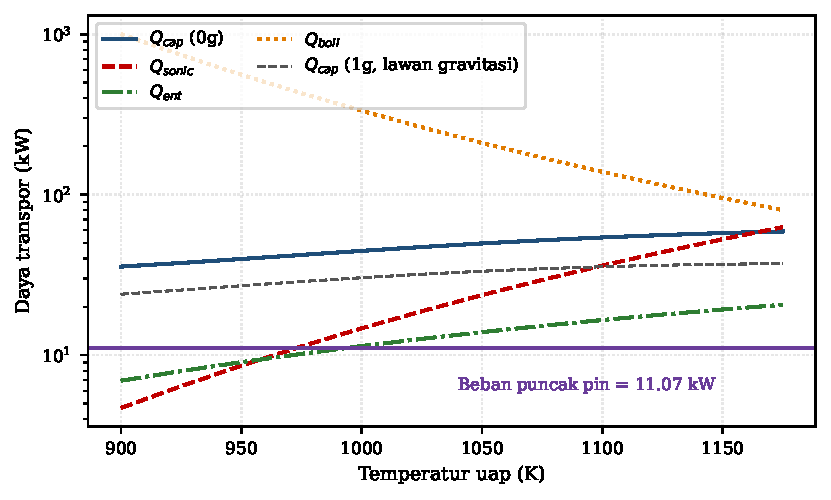
\includegraphics[width=0.72\linewidth,height=\textheight,keepaspectratio]{figures/amplop_operasi.pdf}

}

\caption{\label{fig-amplop}Amplop batas operasi pipa kalor natrium OD 18
mm pada mikrogravitasi (garis penuh) dan pada pengujian darat melawan
gravitasi (garis putus-putus abu-abu). Garis ungu menandai beban puncak
pin ISR.}

\end{figure}%

Tiga rezim terbaca jelas dari gambar tersebut. Pada temperatur di bawah
950 K, batas sonik dan batas viskos mendominasi: pada 900 K, tekanan uap
jenuh hanya 11 kPa sehingga densitas uap sangat rendah dan daya transpor
terbatas pada 4,68 kW. Rezim ini relevan bukan untuk operasi nominal,
melainkan untuk penyalaan, ketika pipa harus melewati temperatur rendah
sebelum mencapai kondisi kerja. Karena itu prosedur penyalaan bertahap
(\emph{controlled startup}) tetap diperlukan meskipun reaktor dirancang
beroperasi pada 1075 K.

Pada rentang 1000--1150 K, batas yang menentukan adalah entrainment,
bukan kapiler. Pada 1075 K, batas kapiler mencapai 51,97 kW sedangkan
batas entrainment hanya 15,22 kW; artinya sumbu masih sanggup
membangkitkan tekanan kapiler yang jauh lebih besar daripada yang
dibutuhkan, tetapi uap yang bergerak dengan kecepatan 133 m/s di atas
permukaan meniskus berpori 15 µm sudah cukup untuk menyeret tetesan
cairan. Batas pendidihan sangat tinggi (169,8 kW) karena konduktivitas
natrium cair yang besar mencegah terbentuknya superheat berarti pada
dinding sumbu.

Temuan ini membalik asumsi yang lazim dipakai pada kajian pipa kalor
logam cair, yang biasanya menempatkan batas kapiler sebagai pembatas
utama pada temperatur tinggi. Penjelasannya bersifat geometris: pipa
in-pin terpaksa berdiameter kecil karena harus masuk ke rongga pin,
sehingga luas penampang uapnya kecil dan kecepatan uapnya tinggi. Pada
pipa berdiameter besar, urutan batas akan kembali seperti biasa. Karena
itu pernyataan ``batas kapiler adalah pembatas'' tidak berlaku umum; ia
bergantung pada rasio antara luas penampang uap dan daya yang dibawa,
yang pada desain in-pin justru tidak menguntungkan.

Pengaruh gravitasi tampak pada kurva putus-putus. Pada 1075 K, batas
kapiler turun dari 51,97 kW pada \(0g\) menjadi 34,54 kW pada \(1g\)
dengan evaporator di atas, yaitu penurunan 34\%. Penurunan ini berasal
dari head hidrostatik 3,4 kPa yang harus dilawan cairan, sebanding
dengan 20\% tekanan kapiler maksimum. Sebaliknya, batas entrainment dan
sonik tidak berubah karena keduanya tidak bergantung pada gravitasi.
Implikasinya praktis: pengujian pipa kalor ISR di laboratorium Bumi pada
orientasi terburuk akan menunjukkan batas sekitar 34 kW, sedangkan
operasi di orbit akan memberikan batas 52 kW. Pengujian darat karena itu
konservatif, tetapi tidak boleh dipakai untuk menyimpulkan kegagalan
desain pada kondisi antariksa.

\section{Profil Aksial pada Beban
Puncak}\label{profil-aksial-pada-beban-puncak}

Gambar 5.3 menampilkan profil tekanan, bilangan Mach, dan tekanan
kapiler pada pin pusat dengan daya 11,07 kWth.

\begin{figure}[htbp]

\centering{

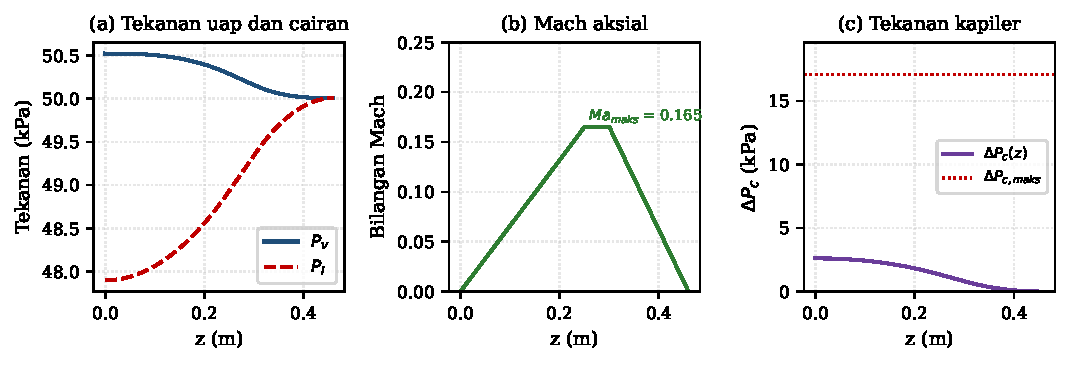
\includegraphics[width=1\linewidth,height=\textheight,keepaspectratio]{figures/profil_detail.pdf}

}

\caption{\label{fig-profil}Profil aksial pada pin beban puncak: (a)
tekanan uap dan tekanan cairan; (b) bilangan Mach; (c) tekanan kapiler
lokal dibandingkan tekanan kapiler maksimum.}

\end{figure}%

Tekanan uap turun dari 50,5 kPa di awal evaporator menjadi 50,0 kPa di
akhir kondensor, yaitu rugi total hanya 514 Pa atau sekitar 1\% dari
tekanan absolut. Penurunan kecil ini terjadi karena densitas uap natrium
pada 1075 K sudah cukup tinggi; sebagai perbandingan, pada 900 K rugi
tekanan untuk daya yang sama akan berkali lipat lebih besar. Tekanan
cairan bergerak berlawanan arah: turun dari 50,0 kPa di kondensor
menjadi 47,9 kPa di evaporator, dengan rugi total 2106 Pa. Dengan
demikian tekanan kapiler yang dibutuhkan di evaporator adalah 2621 Pa,
yaitu 15,4\% dari tekanan kapiler maksimum 17,06 kPa; margin tekanan
yang tersedia 84,6\%.

Konsekuensi termalnya adalah perilaku kuasi-isotermal: beda temperatur
saturasi antara evaporator dan kondensor hanya 1,1 K. Inilah keunggulan
intrinsik pipa kalor sebagai penghubung termal, dan alasan mengapa
desain reaktor antariksa dapat mentransfer panas dari teras ke konverter
dengan gradien temperatur yang sangat kecil.

Profil bilangan Mach memperlihatkan bentuk segitiga khas: nol di kedua
ujung karena laju alir massa nol, dan maksimum 0,165 pada akhir zona
adiabatik tempat laju alir massa mencapai puncak sekaligus densitas
mulai menurun. Profil tekanan kapiler memperlihatkan nilai maksimum di
awal evaporator dan menurun menuju nol di ujung kondensor, sesuai dengan
distribusi kebutuhan tekanan sepanjang siklus.

Hambatan termal pipa terurai menjadi tiga komponen: dinding Mo-30Re
\(7,06\times10^{-4}\) K/W, sumbu komposit \(1,28\times10^{-3}\) K/W, dan
uap \(1,18\times10^{-4}\) K/W. Sumbu menyumbang 60\% hambatan total,
yang menunjukkan bahwa perbaikan performa termal harus diarahkan pada
konduktivitas efektif sumbu, bukan pada ketebalan dinding. Dengan
\(k_{eff} \approx 40\) W/(m·K) pada sumbu jenuh natrium, kenaikan
temperatur radial dari dinding dalam ke inti uap adalah 14,2 K pada
beban puncak --- masih wajar, tetapi menjadi penyumbang terbesar beda
temperatur pipa.

\section{Optimasi Geometri Pipa}\label{optimasi-geometri-pipa}

Pemilihan diameter pipa adalah persoalan optimasi dengan dua sasaran
yang berlawanan: diameter besar menaikkan kapasitas termal, tetapi
memakan volume bahan bakar karena pipa harus masuk ke rongga tengah pin.
Sapuan dilakukan pada delapan diameter dari 10 mm hingga 24 mm dengan
tebal dinding, tebal sumbu, permeabilitas, dan jari-jari pori yang
dijaga tetap, sehingga yang berubah hanya luas penampang uap dan
konsekuensinya terhadap volume bahan bakar.

\begin{longtable}[]{@{}
  >{\centering\arraybackslash}p{(\linewidth - 12\tabcolsep) * \real{0.1429}}
  >{\centering\arraybackslash}p{(\linewidth - 12\tabcolsep) * \real{0.1429}}
  >{\centering\arraybackslash}p{(\linewidth - 12\tabcolsep) * \real{0.1429}}
  >{\centering\arraybackslash}p{(\linewidth - 12\tabcolsep) * \real{0.1429}}
  >{\centering\arraybackslash}p{(\linewidth - 12\tabcolsep) * \real{0.1429}}
  >{\centering\arraybackslash}p{(\linewidth - 12\tabcolsep) * \real{0.1429}}
  >{\centering\arraybackslash}p{(\linewidth - 12\tabcolsep) * \real{0.1429}}@{}}
\caption{Pengaruh diameter luar pipa terhadap batas operasi pada 1075 K
dan konsekuensinya pada volume bahan
bakar.}\label{tbl-trade}\tabularnewline
\toprule\noalign{}
\begin{minipage}[b]{\linewidth}\centering
OD (mm)
\end{minipage} & \begin{minipage}[b]{\linewidth}\centering
\(D_v\) (mm)
\end{minipage} & \begin{minipage}[b]{\linewidth}\centering
\(Q_{cap}\) (kW)
\end{minipage} & \begin{minipage}[b]{\linewidth}\centering
\(Q_{sonic}\) (kW)
\end{minipage} & \begin{minipage}[b]{\linewidth}\centering
\(Q_{ent}\) (kW)
\end{minipage} & \begin{minipage}[b]{\linewidth}\centering
SF (-)
\end{minipage} & \begin{minipage}[b]{\linewidth}\centering
Kehilangan UN (\%)
\end{minipage} \\
\midrule\noalign{}
\endfirsthead
\toprule\noalign{}
\begin{minipage}[b]{\linewidth}\centering
OD (mm)
\end{minipage} & \begin{minipage}[b]{\linewidth}\centering
\(D_v\) (mm)
\end{minipage} & \begin{minipage}[b]{\linewidth}\centering
\(Q_{cap}\) (kW)
\end{minipage} & \begin{minipage}[b]{\linewidth}\centering
\(Q_{sonic}\) (kW)
\end{minipage} & \begin{minipage}[b]{\linewidth}\centering
\(Q_{ent}\) (kW)
\end{minipage} & \begin{minipage}[b]{\linewidth}\centering
SF (-)
\end{minipage} & \begin{minipage}[b]{\linewidth}\centering
Kehilangan UN (\%)
\end{minipage} \\
\midrule\noalign{}
\endhead
\bottomrule\noalign{}
\endlastfoot
10 & 6,6 & 8,89 & 6,01 & 3,11 & 0,28 & 4,1 \\
12 & 8,6 & 16,76 & 10,20 & 5,28 & 0,48 & 8,5 \\
14 & 10,6 & 26,89 & 15,50 & 8,02 & 0,72 & 13,7 \\
16 & 12,6 & 38,82 & 21,90 & 11,33 & 1,02 & 19,7 \\
\textbf{18} & 14,6 & 51,97 & 29,41 & 15,22 & 1,37 & 26,4 \\
20 & 16,6 & 65,90 & 38,01 & 19,67 & 1,78 & 34,0 \\
22 & 18,6 & 80,25 & 47,72 & 24,70 & 2,23 & 42,4 \\
24 & 20,6 & 94,73 & 58,54 & 30,29 & 2,74 & 51,5 \\
\end{longtable}

\begin{figure}[htbp]

\centering{

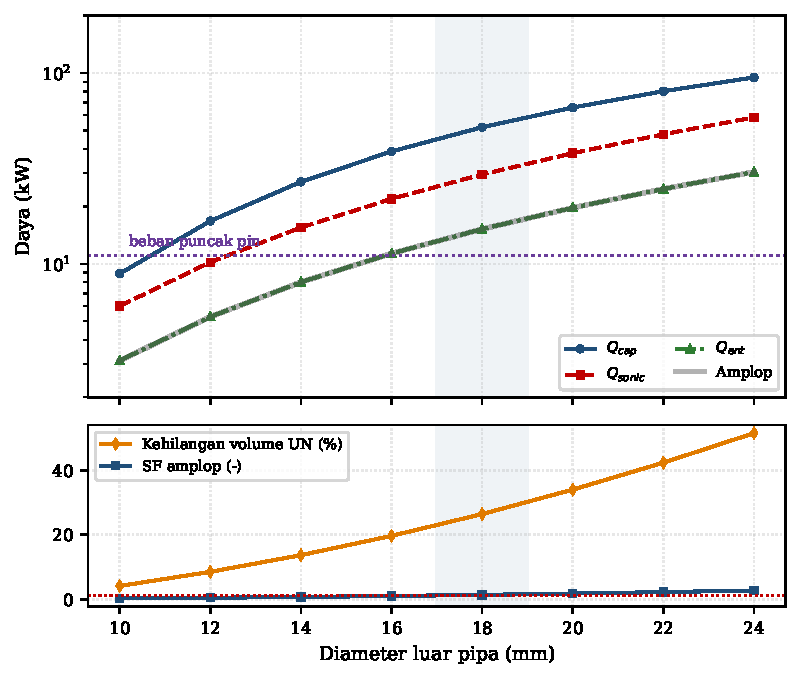
\includegraphics[width=0.7\linewidth,height=\textheight,keepaspectratio]{figures/trade_geometri.pdf}

}

\caption{\label{fig-trade}Pengaruh diameter luar pipa terhadap (atas)
batas-batas operasi pada 1075 K dan (bawah) faktor keselamatan serta
kehilangan volume bahan bakar. Pita biru menandai diameter terpilih.}

\end{figure}%

Hasil sapuan menunjukkan bahwa kapasitas termal naik cepat terhadap
diameter: pada 10 mm amplop hanya 3,11 kW, pada 16 mm 11,33 kW, dan pada
24 mm 30,29 kW. Kenaikan ini berasal dari dua sumber sekaligus, yaitu
luas penampang uap yang bertambah sebanding \(D_v^{2}\) dan densitas uap
yang bertambah karena diameter lebih besar memungkinkan rugi tekanan
lebih kecil. Batas entrainment tetap menjadi pembatas pada seluruh
rentang, dengan batas sonik mendekat pada diameter kecil dan batas
kapiler baru melampaui entrainment pada diameter 10 mm.

Kriteria pemilihan dinyatakan eksplisit: pilih diameter terkecil yang
memberikan \(SF \ge 1{,}3\) pada beban puncak 11,07 kW, karena setiap
milimeter tambahan diameter berarti tambahan kehilangan bahan bakar.
Dengan kriteria itu, diameter 16 mm menghasilkan \(SF = 1{,}02\)
sehingga tidak memenuhi syarat, sedangkan diameter 18 mm menghasilkan
\(SF = 1{,}37\) dengan kehilangan volume bahan bakar 26,4\%. Diameter 20
mm memang memberikan \(SF = 1{,}78\), tetapi kehilangan bahan bakar naik
menjadi 34,0\%, sehingga tambahan margin 30\% harus dibayar dengan
tambahan kehilangan bahan bakar 29\% --- pertukaran yang tidak sepadan
untuk reaktor yang marginnya sudah memadai.

Diameter 18 mm juga memiliki keunggulan praktis. Angka ini dekat dengan
diameter pipa KRUSTY (15,88 mm), sehingga proses pembuatan, pengelasan
ujung, dan pengisian natrium dapat mengacu pada pengalaman manufaktur
yang sudah ada. Dengan tebal dinding 0,9 mm dan tebal sumbu 0,8 mm,
diameter inti uap menjadi 14,6 mm, dan rongga pin yang harus disediakan
adalah 18,2 mm termasuk kelonggaran pemasangan.

\section{Integrasi Teras 61 Pin}\label{integrasi-teras-61-pin}

Distribusi daya radial dibangun dari lima cincin konsentris dengan
faktor puncak 1,28 pada pin pusat hingga 0,81 pada cincin terluar,
dinormalisasi sehingga jumlah daya seluruh pin tepat 500 kWth.
Normalisasi ini penting: tanpa normalisasi, penjumlahan daya cincin
tidak akan sama dengan daya teras, dan kesalahan semacam itu sering
luput pada studi yang hanya mengalikan daya rata-rata dengan faktor
puncak. Dengan normalisasi, daya pin rata-rata menjadi 8,20 kWth dan
daya pin pusat 11,07 kWth, yaitu rasio puncak-terhadap-rata 1,35.

\begin{longtable}[]{@{}
  >{\raggedright\arraybackslash}p{(\linewidth - 20\tabcolsep) * \real{0.0741}}
  >{\centering\arraybackslash}p{(\linewidth - 20\tabcolsep) * \real{0.0926}}
  >{\centering\arraybackslash}p{(\linewidth - 20\tabcolsep) * \real{0.0926}}
  >{\centering\arraybackslash}p{(\linewidth - 20\tabcolsep) * \real{0.0926}}
  >{\centering\arraybackslash}p{(\linewidth - 20\tabcolsep) * \real{0.0926}}
  >{\centering\arraybackslash}p{(\linewidth - 20\tabcolsep) * \real{0.0926}}
  >{\centering\arraybackslash}p{(\linewidth - 20\tabcolsep) * \real{0.0926}}
  >{\centering\arraybackslash}p{(\linewidth - 20\tabcolsep) * \real{0.0926}}
  >{\centering\arraybackslash}p{(\linewidth - 20\tabcolsep) * \real{0.0926}}
  >{\centering\arraybackslash}p{(\linewidth - 20\tabcolsep) * \real{0.0926}}
  >{\centering\arraybackslash}p{(\linewidth - 20\tabcolsep) * \real{0.0926}}@{}}
\caption{Distribusi daya dan keadaan termohidrolika teras ISR 61 pin
pada 500 kWth, \(T_v\) = 1074 K, \(g\) = 0; C1 adalah pin pusat dan C5
adalah cincin terluar.}\label{tbl-teras}\tabularnewline
\toprule\noalign{}
\begin{minipage}[b]{\linewidth}\raggedright
Cincin
\end{minipage} & \begin{minipage}[b]{\linewidth}\centering
\(N\)
\end{minipage} & \begin{minipage}[b]{\linewidth}\centering
\(F_r\)
\end{minipage} & \begin{minipage}[b]{\linewidth}\centering
\(Q_{pin}\) (kW)
\end{minipage} & \begin{minipage}[b]{\linewidth}\centering
\(Q_{cin}\) (kW)
\end{minipage} & \begin{minipage}[b]{\linewidth}\centering
\(T_{clad}\) (K)
\end{minipage} & \begin{minipage}[b]{\linewidth}\centering
\(T_{UN}\) (K)
\end{minipage} & \begin{minipage}[b]{\linewidth}\centering
\(\Delta P_{req}\) (Pa)
\end{minipage} & \begin{minipage}[b]{\linewidth}\centering
\(Ma\)
\end{minipage} & \begin{minipage}[b]{\linewidth}\centering
Margin (\%)
\end{minipage} & \begin{minipage}[b]{\linewidth}\centering
SF
\end{minipage} \\
\midrule\noalign{}
\endfirsthead
\toprule\noalign{}
\begin{minipage}[b]{\linewidth}\raggedright
Cincin
\end{minipage} & \begin{minipage}[b]{\linewidth}\centering
\(N\)
\end{minipage} & \begin{minipage}[b]{\linewidth}\centering
\(F_r\)
\end{minipage} & \begin{minipage}[b]{\linewidth}\centering
\(Q_{pin}\) (kW)
\end{minipage} & \begin{minipage}[b]{\linewidth}\centering
\(Q_{cin}\) (kW)
\end{minipage} & \begin{minipage}[b]{\linewidth}\centering
\(T_{clad}\) (K)
\end{minipage} & \begin{minipage}[b]{\linewidth}\centering
\(T_{UN}\) (K)
\end{minipage} & \begin{minipage}[b]{\linewidth}\centering
\(\Delta P_{req}\) (Pa)
\end{minipage} & \begin{minipage}[b]{\linewidth}\centering
\(Ma\)
\end{minipage} & \begin{minipage}[b]{\linewidth}\centering
Margin (\%)
\end{minipage} & \begin{minipage}[b]{\linewidth}\centering
SF
\end{minipage} \\
\midrule\noalign{}
\endhead
\bottomrule\noalign{}
\endlastfoot
C1 & 1 & 1,28 & 11,07 & 11,07 & 1.096,2 & 1.249,0 & 2.621 & 0,165 & 84,6
& 1,37 \\
C2 & 6 & 1,21 & 10,47 & 62,80 & 1.094,8 & 1.239,3 & 2.457 & 0,156 & 85,6
& 1,45 \\
C3 & 12 & 1,09 & 9,43 & 113,15 & 1.092,6 & 1.222,7 & 2.182 & 0,141 &
87,2 & 1,61 \\
C4 & 18 & 0,93 & 8,04 & 144,81 & 1.089,7 & 1.200,7 & 1.824 & 0,120 &
89,3 & 1,89 \\
C5 & 24 & 0,81 & 7,01 & 168,17 & 1.087,4 & 1.184,1 & 1.562 & 0,105 &
90,8 & 2,17 \\
\textbf{Total} & \textbf{61} & \textbf{1,00} & \textbf{8,20} &
\textbf{500,00} & \textbf{1.096,2} & \textbf{1.249,0} & \textbf{2.621} &
\textbf{0,165} & \textbf{84,6} & \textbf{1,37} \\
\end{longtable}

\begin{figure}[htbp]

\centering{

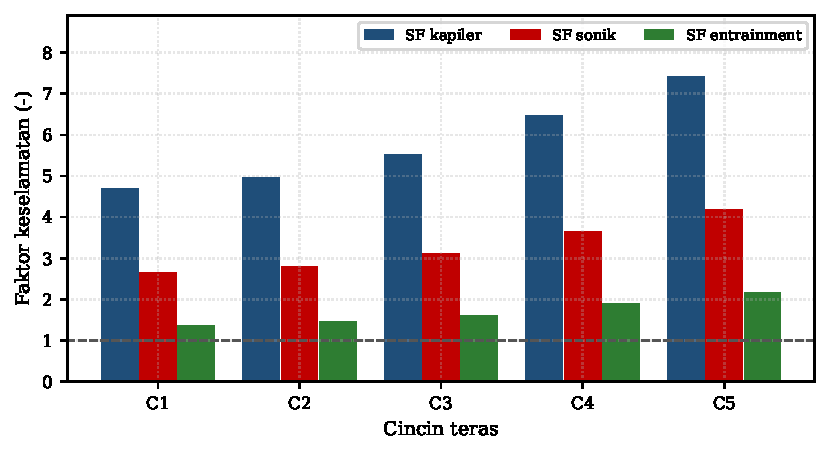
\includegraphics[width=0.7\linewidth,height=\textheight,keepaspectratio]{figures/margin_teras.pdf}

}

\caption{\label{fig-margin}Faktor keselamatan terhadap ketiga batas
dominan pada setiap cincin teras.}

\end{figure}%

Seluruh 61 pin beroperasi dengan faktor keselamatan di atas 1,3. Pin
pusat, yang menjadi kasus terberat, memiliki \(SF = 1{,}37\) terhadap
batas entrainment, 2,66 terhadap batas sonik, dan 4,69 terhadap batas
kapiler. Margin tekanan kapiler pada pin pusat adalah 84,6\%, dan pada
cincin terluar mencapai 90,8\%. Pola ini masuk akal: cincin luar membawa
daya lebih kecil sementara geometri pipanya identik, sehingga marginnya
lebih longgar.

Temperatur dinding kelongsong pada pin pusat mencapai 1096,2 K, yaitu
22,1 K di atas temperatur uap akibat hambatan dinding dan sumbu.
Temperatur puncak bahan bakar mencapai 1249,0 K, dengan kenaikan 152,8 K
di dalam pelet akibat pembangkitan volumetrik 7,71\(\times10^{7}\) W/m³.
Angka ini berada 401 K di bawah batas desain 1650 K, sehingga integritas
bahan bakar tidak menjadi persoalan.

Yang perlu dicatat adalah bahwa kenaikan temperatur di dalam pelet
(152,8 K) jauh lebih besar daripada kenaikan temperatur di dalam pipa
(22,1 K). Ini konsekuensi langsung dari berkurangnya volume bahan bakar:
daya yang sama dibangkitkan dalam volume yang 27\% lebih kecil, sehingga
pembangkitan volumetrik naik 37\% dan gradien temperaturnya ikut naik.
Dengan kata lain, pengecilan volume bahan bakar bukan hanya persoalan
neutronik, tetapi juga menaikkan temperatur bahan bakar pada daya yang
sama.

\section{Toleransi Kegagalan Pipa}\label{toleransi-kegagalan-pipa}

Kegagalan satu pipa kalor adalah skenario yang harus dapat ditanggung
tanpa menyebabkan kerusakan teras. Ketika satu pipa berhenti bekerja,
11,07 kW dari pin tersebut harus mengalir secara lateral melalui blok
kelongsong menuju enam pin tetangga. Dengan konduktansi celah efektif
2000 W/(m²·K) pada luas kontak lateral 0,020 m², hambatan lateralnya
adalah 0,025 K/W, sehingga kenaikan temperatur bahan bakar pin yang
gagal mencapai 277 K dan temperaturnya menjadi 1526 K.

Angka tersebut masih di bawah batas 1650 K, sehingga kegagalan satu pipa
dapat ditoleransi. Beban tambahan pada setiap tetangga adalah 1,85 kW
atau 17,6\% dari daya pin tetangga, sehingga faktor keselamatan tetangga
turun dari 1,37 menjadi 1,18. Nilai ini masih di atas satu, artinya
tetangga tetap beroperasi, tetapi marginnya menipis. Apabila dua pipa
gagal bersamaan, kenaikan temperatur mencapai 554 K dan temperatur bahan
bakar pin yang gagal menjadi 1803 K, melampaui batas 1650 K; skenario
dua kegagalan bersamaan karena itu tidak dapat ditoleransi tanpa
tindakan tambahan.

Kesimpulan ini lebih hati-hati daripada klaim bahwa sistem pipa kalor
``tahan terhadap kegagalan dua pin''. Yang dapat dinyatakan adalah bahwa
satu kegagalan terisolasi dan tidak menjalar, sedangkan dua kegagalan
bersamaan memerlukan strategi mitigasi, misalnya penurunan daya teras
atau peningkatan konduktansi lateral melalui lapisan kontak termal.

\section{Neraca Massa dan Daya
Parasitik}\label{neraca-massa-dan-daya-parasitik}

Perbandingan massa dilakukan dengan menguraikan subsistem pendingin
baseline menjadi komponen-komponen yang dapat diperiksa, bukan dengan
membandingkan dua angka total yang sumbernya tidak jelas.

\begin{longtable}[]{@{}lc@{}}
\caption{Estimasi massa subsistem pendingin teras pada desain baseline
berpompa Na-78K.}\label{tbl-massa-base}\tabularnewline
\toprule\noalign{}
Komponen loop pompa Na-78K & Massa (kg) \\
\midrule\noalign{}
\endfirsthead
\toprule\noalign{}
Komponen loop pompa Na-78K & Massa (kg) \\
\midrule\noalign{}
\endhead
\bottomrule\noalign{}
\endlastfoot
Pompa elektromagnetik (2 unit, 1 cadangan) & 19,00 \\
Pengondisian daya pompa \& kabel & 5,50 \\
Tangki ekspansi \& gas penutup He & 12,00 \\
Perpipaan \& manifold tekanan & 15,00 \\
Inventaris Na-78K (14 L) & 10,50 \\
Instrumentasi aliran \& katup & 3,00 \\
\textbf{Subtotal baseline} & \textbf{65,00} \\
\end{longtable}

\begin{longtable}[]{@{}lc@{}}
\caption{Estimasi massa subsistem pendingin teras pada desain retrofit
61 pipa kalor natrium.}\label{tbl-massa-retr}\tabularnewline
\toprule\noalign{}
Komponen sistem pipa kalor & Massa (kg) \\
\midrule\noalign{}
\endfirsthead
\toprule\noalign{}
Komponen sistem pipa kalor & Massa (kg) \\
\midrule\noalign{}
\endhead
\bottomrule\noalign{}
\endlastfoot
61 pipa kalor Mo-30Re (OD 18 mm, t 0,9 mm) & 15,43 \\
Struktur kasa \& arteri komposit & 1,95 \\
Inventaris natrium (61 pipa) & 0,67 \\
Blok sadel pipa-kondensor \& header & 6,00 \\
\textbf{Subtotal retrofit} & \textbf{24,06} \\
\end{longtable}

\begin{longtable}[]{@{}lc@{}}
\caption{Ringkasan selisih massa subsistem pendingin
teras.}\label{tbl-massa}\tabularnewline
\toprule\noalign{}
Besaran & Nilai \\
\midrule\noalign{}
\endfirsthead
\toprule\noalign{}
Besaran & Nilai \\
\midrule\noalign{}
\endhead
\bottomrule\noalign{}
\endlastfoot
Massa baseline & 65,00 kg \\
Massa retrofit & 24,06 kg \\
\textbf{Selisih bersih} & \textbf{\(-\)}40,94 kg (63,0\%) \\
\end{longtable}

Subsistem pendingin baseline diperkirakan berbobot 65,0 kg, terdiri atas
dua pompa elektromagnetik (satu cadangan), pengondisian daya, tangki
ekspansi dan gas penutup, perpipaan bertekanan, inventaris Na-78K, serta
instrumentasi. Retrofit 61 pipa kalor diperkirakan berbobot 24,1 kg,
terdiri atas selubung Mo-30Re, struktur kasa dan arteri, inventaris
natrium yang jauh lebih kecil, serta blok sadel penghubung ke penukar
kalor. Selisih bersihnya adalah 40,94 kg atau 63,0\% dari massa
subsistem pendingin.

Angka ini perlu dibaca dengan hati-hati karena bergantung pada asumsi
yang dinyatakan. Ketebalan dinding 0,9 mm dipilih dari batas manufaktur,
bukan dari kekuatan; tegangan hoop pada tekanan 50 kPa hanya menuntut
dinding beberapa mikrometer, sehingga dinding 0,5 mm secara teknis layak
dan akan menurunkan massa pipa sekitar 45\%. Sebaliknya, ketidakpastian
pada massa blok sadel dan header bisa mencapai beberapa kilogram. Dengan
rentang asumsi tersebut, penghematan massa subsistem berada pada kisaran
30--45 kg.

\begin{figure}[htbp]

\centering{

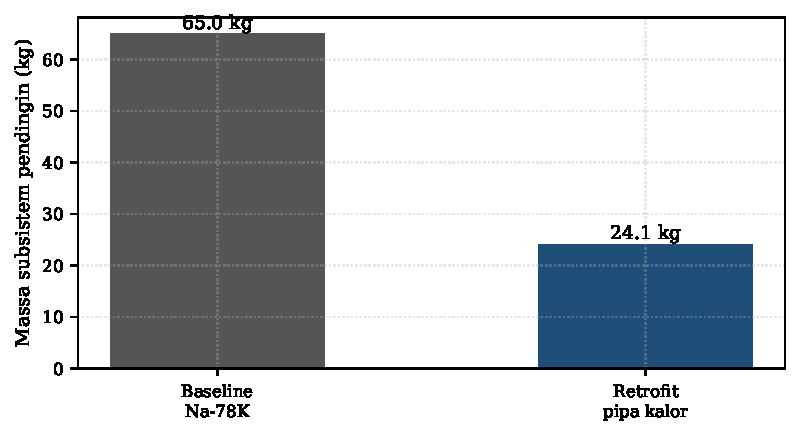
\includegraphics[width=0.62\linewidth,height=\textheight,keepaspectratio]{figures/neraca_massa.pdf}

}

\caption{\label{fig-massa}Perbandingan massa subsistem pendingin antara
loop pompa Na-78K dan sistem 61 pipa kalor.}

\end{figure}%

Daya parasitik pompa dihitung dari kebutuhan hidraulik sebenarnya, bukan
diasumsikan.

\begin{longtable}[]{@{}lcc@{}}
\caption{Estimasi daya pompa elektromagnetik loop Na-78K pada daya teras
500 kWth.}\label{tbl-pompa}\tabularnewline
\toprule\noalign{}
Besaran & Nilai & Satuan \\
\midrule\noalign{}
\endfirsthead
\toprule\noalign{}
Besaran & Nilai & Satuan \\
\midrule\noalign{}
\endhead
\bottomrule\noalign{}
\endlastfoot
Laju alir massa Na-78K & 2,083 & kg/s \\
Tekanan pompa total & 30,000 & kPa \\
Daya hidraulik & 80,128 & W \\
Efisiensi pompa EM & 15,000 & \% \\
Daya listrik pompa & 534,188 & W \\
Fraksi daya termal & 0,107 & \% \\
\end{longtable}

Pada daya teras 500 kWth dengan beda temperatur loop 200 K, laju alir
Na-78K yang dibutuhkan adalah 2,08 kg/s. Dengan rugi tekanan total 30
kPa, daya hidrauliknya hanya 80 W; pada efisiensi pompa elektromagnetik
15\%, daya listrik yang dibutuhkan adalah 534 W atau 0,107\% dari daya
termal. Angka ini jauh lebih kecil daripada asumsi 12,5--18,5 kWe yang
kadang dipakai pada studi sejenis, dan perbedaannya penting: pompa bukan
beban daya yang besar, sehingga penghapusannya tidak memberikan
keuntungan listrik yang dramatis. Keuntungan utama penghapusan pompa
terletak pada keandalan, bukan pada efisiensi.

Perbandingan menyeluruh antara kedua sistem dirangkum pada Tabel 5.10.

\begin{longtable}[]{@{}
  >{\raggedright\arraybackslash}p{(\linewidth - 4\tabcolsep) * \real{0.3333}}
  >{\raggedright\arraybackslash}p{(\linewidth - 4\tabcolsep) * \real{0.3333}}
  >{\raggedright\arraybackslash}p{(\linewidth - 4\tabcolsep) * \real{0.3333}}@{}}
\caption{Perbandingan menyeluruh sistem pendingin teras
ISR.}\label{tbl-perbandingan}\tabularnewline
\toprule\noalign{}
\begin{minipage}[b]{\linewidth}\raggedright
Aspek
\end{minipage} & \begin{minipage}[b]{\linewidth}\raggedright
Baseline Na-78K
\end{minipage} & \begin{minipage}[b]{\linewidth}\raggedright
Retrofit pipa kalor natrium
\end{minipage} \\
\midrule\noalign{}
\endfirsthead
\toprule\noalign{}
\begin{minipage}[b]{\linewidth}\raggedright
Aspek
\end{minipage} & \begin{minipage}[b]{\linewidth}\raggedright
Baseline Na-78K
\end{minipage} & \begin{minipage}[b]{\linewidth}\raggedright
Retrofit pipa kalor natrium
\end{minipage} \\
\midrule\noalign{}
\endhead
\bottomrule\noalign{}
\endlastfoot
Fluida pendingin & Eutektik Na-78K, fase tunggal & Natrium murni, dua
fasa \\
Mekanisme aliran & Pompa elektromagnetik aktif & Tekanan kapiler
pasif \\
Titik didih pada tekanan operasi & \$\pm\$1000 K & 1156 K pada 1 atm \\
Temperatur kerja teras & 750 K masuk / 950 K keluar & 1074 K
isotermal \\
Daya parasitik & 0,53 kW & 0 \\
Massa subsistem & 65,0 kg & 24,1 kg \\
Getaran mekanik & Ada, dari pulsasi pompa & Tidak ada \\
Modus kegagalan & Pompa macet berujung kehilangan pendinginan teras &
Satu pipa gagal bersifat lokal \\
Pembuangan panas peluruhan & Memerlukan daya cadangan & Berlangsung
pasif \\
Konsekuensi pada bahan bakar & Tidak ada & Volume UN berkurang 27,2\% \\
\end{longtable}

\section{Pembahasan: Harga Bahan Bakar dan Batas
Kesimpulan}\label{pembahasan-harga-bahan-bakar-dan-batas-kesimpulan}

Keuntungan massa dan keselamatan di atas harus dibayar dengan bahan
bakar. Melebarkan rongga tengah pin dari 7,65 mm menjadi 18,2 mm
mengurangi luas annulus bahan bakar dari 788,8 mm² menjadi 574,2 mm²,
sehingga volume uranium nitrida per pin turun dari 197,2 cm³ menjadi
143,6 cm³.

\begin{longtable}[]{@{}lcc@{}}
\caption{Konsekuensi geometri pipa 18 mm terhadap inventaris bahan bakar
dan umur teras.}\label{tbl-bahan-bakar}\tabularnewline
\toprule\noalign{}
Besaran & Nilai & Satuan \\
\midrule\noalign{}
\endfirsthead
\toprule\noalign{}
Besaran & Nilai & Satuan \\
\midrule\noalign{}
\endhead
\bottomrule\noalign{}
\endlastfoot
Volume UN per pin baseline & 197,18 & cm³ \\
Volume UN per pin retrofit & 143,63 & cm³ \\
Massa UN baseline (61 pin) & 154,83 & kg \\
Massa UN retrofit (61 pin) & 112,78 & kg \\
Kehilangan UN & 27,16 & \% \\
Umur teras ekuivalen & 12,38 & tahun \\
Tinggi aktif untuk paritas volume & 343,20 & mm \\
\end{longtable}

Total massa UN untuk 61 pin turun dari 154,83 kg menjadi 112,78 kg,
yaitu kehilangan 27,16\%. Karena umur teras sebanding dengan inventaris
fisil dibagi daya, kehilangan ini secara langsung memangkas umur dari 17
tahun menjadi sekitar 12,4 tahun apabila daya dan pengayaan
dipertahankan. Untuk memulihkan volume bahan bakar pada diameter pin
yang sama, tinggi aktif harus dinaikkan dari 250 mm menjadi 343 mm;
alternatifnya adalah menaikkan pengayaan, yang tidak dievaluasi di sini
karena berada di luar lingkup termohidrolika.

Dengan demikian gambaran akhirnya lebih berimbang daripada narasi yang
biasa muncul pada studi pipa kalor. Jika tinggi aktif dipertahankan,
massa reaktor turun karena dua sebab sekaligus --- penghematan subsistem
40,94 kg dan pengurangan bahan bakar 42,05 kg --- tetapi sebagian
penurunan itu adalah konsekuensi umur teras yang lebih pendek, bukan
efisiensi desain. Jika tinggi aktif dinaikkan untuk mempertahankan umur,
massa bahan bakar kembali dan massa bejana serta reflektor bertambah,
sehingga penghematan bersih menyusut menjadi orde 10--25 kg. Manfaat
yang tidak menyusut adalah hilangnya komponen bergerak, hilangnya daya
parasitik, dan degradasi bertahap ketika satu pipa gagal.

Beberapa keterbatasan perlu dinyatakan agar kesimpulan tidak dibaca
melebihi dukungannya. Pertama, model bersifat tunak sehingga tidak dapat
menilai perilaku penyalaan, pembekuan natrium, atau transien daya;
padahal justru pada transien penyalaan batas sonik dan viskos paling
kritis. Kedua, aliran uap diselesaikan satu dimensi dengan asumsi
saturasi lokal, sehingga fenomena tiga dimensi seperti resirkulasi di
ujung kondensor dan ketidakseragaman film kondensat tidak tertangkap.
Ketiga, kriteria entrainment yang dipakai adalah kriteria Weber klasik;
kriteria ini diketahui terlalu konservatif untuk pori sangat halus dan
terlalu longgar untuk permukaan kasa yang tidak seragam, sehingga margin
1,37 sebaiknya dibaca sebagai indikasi orde besaran, bukan angka pasti.

Keempat, data validasi KRUSTY berjumlah lima titik dan mencakup rentang
daya yang lebih rendah daripada daya pin ISR; ekstrapolasi ke 11 kW per
pipa adalah ekstrapolasi faktor sebelas, sehingga validasi pada daya
tinggi masih menuntut pengujian tersendiri. Kelima, analisis neutronik
tidak dilakukan, padahal kehilangan 27\% bahan bakar pasti mengubah
reaktivitas dan koefisien umpan balik; angka umur 12,4 tahun hanyalah
perkiraan skala.

Keterbatasan itu tidak membatalkan kesimpulan utama, tetapi menentukan
cara membacanya: model ini adalah alat penyaring desain yang telah
diverifikasi dan divalidasi pada rentang terbatas, bukan pengganti
pengujian.

\chapter{KESIMPULAN DAN SARAN}\label{kesimpulan-dan-saran}

\section{Kesimpulan}\label{kesimpulan}

Berdasarkan hasil verifikasi, validasi, dan penerapan model, dapat
disimpulkan sebagai berikut.

\begin{enumerate}
\def\labelenumi{\arabic{enumi}.}
\item
  Model tereduksi satu dimensi aliran dua fasa berhasil dibangun dengan
  menyelesaikan momentum uap kompresibel secara \emph{marching},
  filtrasi Darcy pada sumbu komposit, lima batas operasi, dan jaringan
  hambatan termal. Verifikasi menunjukkan konvergensi grid 0,03\% pada
  240 titik, kesesuaian 0,02\% dengan solusi Darcy analitik untuk aliran
  cairan, kesesuaian 0,25\% dengan solusi Hagen--Poiseuille untuk aliran
  uap, dan deviasi di bawah 0,6\% terhadap nilai rujukan sifat
  termofisika natrium.
\item
  Validasi terhadap lima kondisi tunak uji KRUSTY dengan protokol
  \emph{leave-one-out} menghasilkan MAPE 4,68\%, RMSE 2,08 K, dan
  \(R^{2} = 0{,}961\), dengan galat terbesar 6,29\% pada daya tertinggi.
  Hambatan antarmuka hasil kalibrasi, 0,0384 K/W, berada di dalam
  rentang yang diperkirakan secara independen dari konduktansi kontak
  logam, sehingga parameter kalibrasi memiliki dasar fisik.
\item
  Hambatan termal intrinsik pipa kalor natrium KRUSTY hanya
  4,4--5,0\(\times10^{-3}\) K/W, sehingga hampir seluruh beda temperatur
  26--56 K yang terukur berasal dari antarmuka pengujian, bukan dari
  pipa. Temuan ini menjelaskan mengapa model tanpa parameter antarmuka
  tidak dapat mencocokkan data uji secara langsung, dan mengapa klaim
  akurasi di bawah 1\% pada studi sejenis perlu dicurigai.
\item
  Pada rentang temperatur kerja 1000--1150 K, mekanisme pembatas pipa
  kalor in-pin berdiameter luar 16--20 mm adalah batas entrainment,
  bukan batas kapiler. Pada 1075 K, batas entrainment 15,22 kW jauh
  lebih rendah daripada batas kapiler 51,97 kW dan batas sonik 29,41 kW.
  Penyebabnya adalah luas penampang uap yang kecil akibat batasan
  geometri pin, yang menaikkan kecepatan uap hingga 133 m/s pada beban
  puncak.
\item
  Mikrogravitasi menaikkan batas kapiler sebesar 50\% dibandingkan
  pengujian darat melawan gravitasi (51,97 kW berbanding 34,54 kW pada
  1075 K), tetapi tidak mengubah batas entrainment maupun sonik.
  Pengujian darat karena itu konservatif untuk batas kapiler, namun
  tidak mewakili kondisi operasi sesungguhnya.
\item
  Diameter luar 18 mm merupakan diameter terkecil yang memenuhi kriteria
  \(SF \ge 1{,}3\) pada beban puncak 11,07 kW, dengan \(SF = 1{,}37\),
  margin tekanan kapiler 84,6\%, dan temperatur puncak bahan bakar 1249
  K. Diameter 16 mm gagal memenuhi kriteria (\(SF = 1{,}02\)), sedangkan
  diameter 20 mm menaikkan margin menjadi 1,78 tetapi menambah
  kehilangan bahan bakar dari 26,4\% menjadi 34,0\%.
\item
  Seluruh 61 pin teras ISR 500 kWth dapat didinginkan secara pasif,
  dengan faktor keselamatan antara 1,37 pada pin pusat hingga 2,17 pada
  cincin terluar. Kegagalan satu pipa menaikkan temperatur bahan bakar
  pin yang gagal menjadi 1526 K dan menurunkan faktor keselamatan
  tetangga menjadi 1,18, sehingga masih dapat ditoleransi; kegagalan dua
  pipa bersamaan menaikkan temperatur menjadi 1803 K dan melampaui batas
  desain.
\item
  Retrofit pipa kalor memangkas massa subsistem pendingin dari 65,0 kg
  menjadi 24,1 kg, yaitu penghematan 40,94 kg atau 63,0\%, serta
  menghilangkan daya parasitik pompa sebesar 0,53 kW. Namun retrofit
  juga mengurangi volume bahan bakar 27,2\% dan menurunkan umur teras
  dari 17 tahun menjadi sekitar 12,4 tahun; apabila umur dipulihkan
  dengan menaikkan tinggi aktif menjadi 343 mm, penghematan massa bersih
  menyusut menjadi orde 10--25 kg. Manfaat utama rancangan ini adalah
  keselamatan inheren dan degradasi bertahap, bukan penghematan massa.
\end{enumerate}

\section{Saran}\label{saran}

Beberapa saran untuk penelitian lanjutan disusun berdasarkan
keterbatasan yang ditemukan.

\begin{enumerate}
\def\labelenumi{\arabic{enumi}.}
\item
  Model perlu diperluas menjadi kuasi-transien agar dapat menilai
  penyalaan dari kondisi beku, pembekuan kondensat, dan respons terhadap
  perubahan daya, karena justru pada transien itulah batas sonik dan
  viskos menjadi kritis.
\item
  Validasi sebaiknya dilengkapi dengan data pipa kalor berdaya di atas 5
  kW per pipa, misalnya dari uji pipa kalor natrium skala penuh, karena
  penerapan pada ISR melibatkan ekstrapolasi daya sebesar faktor sebelas
  dari rentang validasi.
\item
  Kriteria entrainment perlu diuji ulang secara eksperimental untuk pori
  berukuran 10--30 µm pada temperatur 1000--1150 K, mengingat justru
  kriteria inilah yang menentukan margin desain, sementara dasar
  empirisnya masih berasal dari percobaan air pada temperatur rendah.
\item
  Analisis neutronik penuh perlu dilakukan untuk mengevaluasi
  konsekuensi pengurangan 27\% volume bahan bakar terhadap reaktivitas,
  distribusi fluks, koefisien umpan balik, dan umur teras; hasil pada
  skripsi ini hanya perkiraan skala berdasarkan kesebandingan inventaris
  fisil.
\item
  Alternatif arsitektur perlu dikaji, khususnya penempatan pipa kalor
  pada ruang antar-pin dengan pitch yang diperbesar, atau kombinasi pipa
  kalor in-pin dengan penurunan daya per pin, agar kehilangan bahan
  bakar dapat ditekan tanpa mengorbankan margin termal.
\item
  Evaluasi termomekanik kelongsong Mo-30Re perlu dilakukan, karena
  gradien temperatur 153 K di dalam pelet dan tegangan akibat tekanan
  uap natrium 50 kPa belum diperhitungkan dalam penelitian ini.
\end{enumerate}

\chapter*{DAFTAR PUSTAKA}\label{daftar-pustaka}
\addcontentsline{toc}{chapter}{DAFTAR PUSTAKA}

\protect\phantomsection\label{refs}
\begin{CSLReferences}{0}{1}
\bibitem[\citeproctext]{ref-elgenk2009deployment}
\CSLLeftMargin{{[}1{]} }%
\CSLRightInline{M. S. El-Genk. {``Deployment history and design
considerations for space reactor power systems''} \emph{Acta
Astronautica}, vol. 64, no. 7-8, pp. 833-849, 2009.}

\bibitem[\citeproctext]{ref-un1992principles}
\CSLLeftMargin{{[}2{]} }%
\CSLRightInline{United Nations General Assembly. \emph{Principles
Relevant to the Use of Nuclear Power Sources in Outer Space}. 1992.}

\bibitem[\citeproctext]{ref-king2006submersion}
\CSLLeftMargin{{[}3{]} }%
\CSLRightInline{J. C. King dan M. S. El-Genk.
{``\href{https://doi.org/10.1016/j.nucengdes.2005.12.010}{Submersion-subcritical
safe space (S4) reactor}''} \emph{Nuclear Engineering and Design}, vol.
236, no. 17, pp. 1759-1777, 2006.}

\bibitem[\citeproctext]{ref-elgenk2004sair}
\CSLLeftMargin{{[}4{]} }%
\CSLRightInline{M. S. El-Genk dan J.-M. P. Tournier.
{``\href{https://doi.org/10.1016/j.pnucene.2004.08.002}{SAIR - scalable
AMTEC integrated reactor space power system}''} \emph{Progress in
Nuclear Energy}, vol. 45, no. 1, pp. 25-69, 2004.}

\bibitem[\citeproctext]{ref-cotter1967theory}
\CSLLeftMargin{{[}5{]} }%
\CSLRightInline{T. P. Cotter. \emph{Theory of Heat Pipes}. Los Alamos,
NM, Los Alamos Scientific Laboratory, 1967.}

\bibitem[\citeproctext]{ref-faghri1995heat}
\CSLLeftMargin{{[}6{]} }%
\CSLRightInline{A. Faghri. \emph{Heat Pipe Science and Technology}.
Washington, DC, Taylor \& Francis, 1995.}

\bibitem[\citeproctext]{ref-poston2000heatpipe}
\CSLLeftMargin{{[}7{]} }%
\CSLRightInline{D. I. Poston. \emph{The Heatpipe-Operated Mars
Exploration Reactor (HOMER)}. Los Alamos, NM, Los Alamos National
Laboratory, 2000.}

\bibitem[\citeproctext]{ref-briggs2018electrically}
\CSLLeftMargin{{[}8{]} }%
\CSLRightInline{M. H. Briggs, M. A. Gibson dan J. L. Sanzi.
\emph{Electrically Heated Testing of the Kilowatt Reactor Using Stirling
TechnologY (KRUSTY) Experiment Using a Depleted Uranium Core}. NASA
Technical Memorandum, Cleveland, Ohio, National Aeronautics; Space
Administration (NASA), 2018.}

\bibitem[\citeproctext]{ref-gibson2018krusty}
\CSLLeftMargin{{[}9{]} }%
\CSLRightInline{M. A. Gibson, D. I. Poston, P. R. McClure, J. L. Sanzi
dan M. H. Briggs.
{``\href{https://doi.org/10.1080/00295450.2020.1725740}{NASA's Kilopower
Reactor Using Stirling Technology (KRUSTY) Ground Test Overview and
Results}''} \emph{Nuclear Technology}, vol. 206, no. sup1, pp. S1-S15,
2020.}

\bibitem[\citeproctext]{ref-dunn2012heat}
\CSLLeftMargin{{[}10{]} }%
\CSLRightInline{P. D. Dunn dan D. A. Reay. \emph{Heat Pipes}. Oxford,
UK, Butterworth-Heinemann, 2012.}

\bibitem[\citeproctext]{ref-khandaq2020conceptual}
\CSLLeftMargin{{[}11{]} }%
\CSLRightInline{M. F. Khandaq, A. W. Harto dan A. Agung.
{``\href{https://doi.org/10.1016/j.pnucene.2019.103109}{Conceptual core
design study for Indonesian Space Reactor (ISR)}''} \emph{Progress in
Nuclear Energy}, vol. 118, pp. 103109, 2020.}

\bibitem[\citeproctext]{ref-fink1995thermodynamic}
\CSLLeftMargin{{[}12{]} }%
\CSLRightInline{J. K. Fink dan L. Leibowitz. \emph{Thermodynamic and
Transport Properties of Sodium Liquid and Vapor}. Argonne, IL, Argonne
National Laboratory, 1995.}

\bibitem[\citeproctext]{ref-busse1973theory}
\CSLLeftMargin{{[}13{]} }%
\CSLRightInline{C. A. Busse.
{``\href{https://doi.org/10.1016/0017-9310(73)90044-6}{Theory of the
Ultimate Heat Transfer Limit of Cylindrical Heat Pipes}''}
\emph{International Journal of Heat and Mass Transfer}, vol. 16, no. 1,
pp. 169-186, 1973.}

\bibitem[\citeproctext]{ref-chi1976heat}
\CSLLeftMargin{{[}14{]} }%
\CSLRightInline{S. W. Chi. \emph{Heat Pipe Theory and Practice: A
Sourcebook}. Washington, DC, Hemisphere Publishing Corporation, 1976.}

\bibitem[\citeproctext]{ref-foust1972sodium}
\CSLLeftMargin{{[}15{]} }%
\CSLRightInline{O. J. Foust. \emph{Sodium-NaK Engineering Handbook:
Volume 1 - Physical and Chemical Properties}. New York, Gordon; Breach
Science Publishers, 1972.}

\end{CSLReferences}

\chapter*{LAMPIRAN A: LISTING KODE
PROGRAM}\label{lampiran-a-listing-kode-program}
\addcontentsline{toc}{chapter}{LAMPIRAN A: LISTING KODE PROGRAM}

Lampiran ini memuat inti kode model tereduksi yang menghasilkan seluruh
angka pada Bab V. Kode lengkap beserta skrip studi tersedia pada folder
\emph{src} di repositori skripsi. Berkas \emph{hp\_model.py} berisi
sifat termofisika, geometri, penyelesai aksial, batas operasi, dan
jaringan hambatan termal, sedangkan berkas \emph{run\_all.py}
menghasilkan seluruh tabel dan gambar.

\begin{Shaded}
\begin{Highlighting}[]
\CommentTok{"""Kutipan inti hp\_model.py; berkas lengkap tersedia pada folder src."""}

\CommentTok{\# {-}{-}{-} Sifat natrium: panas laten, tekanan uap jenuh, temperatur saturasi {-}{-}{-}}
\KeywordTok{def}\NormalTok{ h\_fg(T: }\BuiltInTok{float}\NormalTok{) }\OperatorTok{{-}\textgreater{}} \BuiltInTok{float}\NormalTok{:}
    \CommentTok{"""Panas laten penguapan natrium [J/kg], Fink \& Leibowitz (1995)."""}
\NormalTok{    x }\OperatorTok{=} \BuiltInTok{max}\NormalTok{(}\FloatTok{1.0e{-}6}\NormalTok{, }\FloatTok{1.0} \OperatorTok{{-}}\NormalTok{ T }\OperatorTok{/}\NormalTok{ T\_CRIT)}
    \ControlFlowTok{return} \FloatTok{4.76e6} \OperatorTok{*}\NormalTok{ x }\OperatorTok{**} \FloatTok{0.38}


\KeywordTok{def}\NormalTok{ \_build\_psat\_table() }\OperatorTok{{-}\textgreater{}} \BuiltInTok{tuple}\NormalTok{[np.ndarray, np.ndarray]:}
    \CommentTok{"""Integrasi Clausius{-}Clapeyron dari titik didih normal.}

\CommentTok{    d(ln P)/dT = h\_fg(T) / (R\_g T\^{}2)}

\CommentTok{    Integrasi numeris (aturan trapesium) pada grid halus, dua arah dari}
\CommentTok{    T\_BOIL. Hasilnya konsisten secara termodinamika dengan h\_fg(T) yang}
\CommentTok{    dipakai model, sehingga tidak ada inkonsistensi P\_sat vs h\_fg.}
\CommentTok{    """}
\NormalTok{    Ts }\OperatorTok{=}\NormalTok{ np.arange(}\FloatTok{400.0}\NormalTok{, }\FloatTok{1500.0} \OperatorTok{+} \FloatTok{0.25}\NormalTok{, }\FloatTok{0.25}\NormalTok{)}
\NormalTok{    lnP }\OperatorTok{=}\NormalTok{ np.empty\_like(Ts)}
\NormalTok{    i0 }\OperatorTok{=} \BuiltInTok{int}\NormalTok{(np.argmin(np.}\BuiltInTok{abs}\NormalTok{(Ts }\OperatorTok{{-}}\NormalTok{ T\_BOIL)))}
\NormalTok{    lnP[i0] }\OperatorTok{=}\NormalTok{ math.log(P\_ATM)}
    \CommentTok{\# ke atas}
    \ControlFlowTok{for}\NormalTok{ i }\KeywordTok{in} \BuiltInTok{range}\NormalTok{(i0 }\OperatorTok{+} \DecValTok{1}\NormalTok{, }\BuiltInTok{len}\NormalTok{(Ts)):}
\NormalTok{        T1, T2 }\OperatorTok{=}\NormalTok{ Ts[i }\OperatorTok{{-}} \DecValTok{1}\NormalTok{], Ts[i]}
\NormalTok{        f }\OperatorTok{=} \KeywordTok{lambda}\NormalTok{ T: h\_fg(T) }\OperatorTok{/}\NormalTok{ (R\_G }\OperatorTok{*}\NormalTok{ T }\OperatorTok{*}\NormalTok{ T)}
\NormalTok{        lnP[i] }\OperatorTok{=}\NormalTok{ lnP[i }\OperatorTok{{-}} \DecValTok{1}\NormalTok{] }\OperatorTok{+} \FloatTok{0.5} \OperatorTok{*}\NormalTok{ (f(T1) }\OperatorTok{+}\NormalTok{ f(T2)) }\OperatorTok{*}\NormalTok{ (T2 }\OperatorTok{{-}}\NormalTok{ T1)}
    \CommentTok{\# ke bawah}
    \ControlFlowTok{for}\NormalTok{ i }\KeywordTok{in} \BuiltInTok{range}\NormalTok{(i0 }\OperatorTok{{-}} \DecValTok{1}\NormalTok{, }\OperatorTok{{-}}\DecValTok{1}\NormalTok{, }\OperatorTok{{-}}\DecValTok{1}\NormalTok{):}
\NormalTok{        T1, T2 }\OperatorTok{=}\NormalTok{ Ts[i], Ts[i }\OperatorTok{+} \DecValTok{1}\NormalTok{]}
\NormalTok{        f }\OperatorTok{=} \KeywordTok{lambda}\NormalTok{ T: h\_fg(T) }\OperatorTok{/}\NormalTok{ (R\_G }\OperatorTok{*}\NormalTok{ T }\OperatorTok{*}\NormalTok{ T)}
\NormalTok{        lnP[i] }\OperatorTok{=}\NormalTok{ lnP[i }\OperatorTok{+} \DecValTok{1}\NormalTok{] }\OperatorTok{{-}} \FloatTok{0.5} \OperatorTok{*}\NormalTok{ (f(T1) }\OperatorTok{+}\NormalTok{ f(T2)) }\OperatorTok{*}\NormalTok{ (T2 }\OperatorTok{{-}}\NormalTok{ T1)}
    \ControlFlowTok{return}\NormalTok{ Ts, lnP}


\NormalTok{\_TS, \_LNP }\OperatorTok{=}\NormalTok{ \_build\_psat\_table()}


\KeywordTok{def}\NormalTok{ psat(T: }\BuiltInTok{float}\NormalTok{) }\OperatorTok{{-}\textgreater{}} \BuiltInTok{float}\NormalTok{:}
    \CommentTok{"""Tekanan uap jenuh natrium [Pa]."""}
    \ControlFlowTok{return} \BuiltInTok{float}\NormalTok{(np.exp(np.interp(T, \_TS, \_LNP)))}


\KeywordTok{def}\NormalTok{ tsat(P: }\BuiltInTok{float}\NormalTok{) }\OperatorTok{{-}\textgreater{}} \BuiltInTok{float}\NormalTok{:}
    \CommentTok{"""Temperatur saturasi natrium [K] dari tekanan [Pa]."""}
    \ControlFlowTok{return} \BuiltInTok{float}\NormalTok{(np.interp(math.log(}\BuiltInTok{max}\NormalTok{(P, }\FloatTok{1e{-}6}\NormalTok{)), \_LNP, \_TS))}

\CommentTok{\# ...}

\CommentTok{\# {-}{-}{-} Geometri pipa kalor dan properti turunannya {-}{-}{-}}
\AttributeTok{@dataclass}
\KeywordTok{class}\NormalTok{ HeatPipe:}
    \CommentTok{"""Geometri pipa kalor (semua panjang dalam meter)."""}
\NormalTok{    name: }\BuiltInTok{str}
\NormalTok{    L\_e: }\BuiltInTok{float}          \CommentTok{\# panjang evaporator}
\NormalTok{    L\_a: }\BuiltInTok{float}          \CommentTok{\# panjang adiabatik}
\NormalTok{    L\_c: }\BuiltInTok{float}          \CommentTok{\# panjang kondensor}
\NormalTok{    r\_o: }\BuiltInTok{float}          \CommentTok{\# jari{-}jari luar selubung}
\NormalTok{    t\_wall: }\BuiltInTok{float}       \CommentTok{\# tebal dinding selubung}
\NormalTok{    t\_wick: }\BuiltInTok{float}       \CommentTok{\# tebal sumbu (annular)}
\NormalTok{    r\_eff: }\BuiltInTok{float}        \CommentTok{\# jari{-}jari pori efektif meniskus}
\NormalTok{    K: }\BuiltInTok{float}            \CommentTok{\# permeabilitas sumbu [m2]}
\NormalTok{    eps: }\BuiltInTok{float}          \CommentTok{\# porositas sumbu ({-})}
\NormalTok{    k\_wall: }\BuiltInTok{float}       \CommentTok{\# konduktivitas selubung [W/(m K)]}
\NormalTok{    rho\_wall: }\BuiltInTok{float}     \CommentTok{\# densitas selubung [kg/m3]}
\NormalTok{    k\_solid: }\BuiltInTok{float} \OperatorTok{=} \FloatTok{15.0}   \CommentTok{\# konduktivitas material kasa [W/(m K)]}
\NormalTok{    r\_n: }\BuiltInTok{float} \OperatorTok{=} \FloatTok{2.5e{-}6}     \CommentTok{\# jari{-}jari rongga nukleasi [m]}
\NormalTok{    fill\_frac: }\BuiltInTok{float} \OperatorTok{=} \FloatTok{0.35}  \CommentTok{\# fraksi area annulus yang terbuka untuk aliran}

    \CommentTok{\# {-}{-}{-} properti turunan {-}{-}{-}{-}{-}{-}{-}{-}{-}{-}{-}{-}{-}{-}{-}{-}{-}{-}{-}{-}{-}{-}{-}{-}{-}{-}{-}{-}{-}{-}{-}{-}{-}{-}{-}{-}{-}{-}{-}{-}{-}{-}{-}{-}{-}{-}{-}{-}{-}}
    \AttributeTok{@property}
    \KeywordTok{def}\NormalTok{ L(}\VariableTok{self}\NormalTok{) }\OperatorTok{{-}\textgreater{}} \BuiltInTok{float}\NormalTok{:}
        \ControlFlowTok{return} \VariableTok{self}\NormalTok{.L\_e }\OperatorTok{+} \VariableTok{self}\NormalTok{.L\_a }\OperatorTok{+} \VariableTok{self}\NormalTok{.L\_c}

    \AttributeTok{@property}
    \KeywordTok{def}\NormalTok{ r\_i(}\VariableTok{self}\NormalTok{) }\OperatorTok{{-}\textgreater{}} \BuiltInTok{float}\NormalTok{:}
        \ControlFlowTok{return} \VariableTok{self}\NormalTok{.r\_o }\OperatorTok{{-}} \VariableTok{self}\NormalTok{.t\_wall}

    \AttributeTok{@property}
    \KeywordTok{def}\NormalTok{ r\_v(}\VariableTok{self}\NormalTok{) }\OperatorTok{{-}\textgreater{}} \BuiltInTok{float}\NormalTok{:}
        \ControlFlowTok{return} \VariableTok{self}\NormalTok{.r\_i }\OperatorTok{{-}} \VariableTok{self}\NormalTok{.t\_wick}

    \AttributeTok{@property}
    \KeywordTok{def}\NormalTok{ D\_v(}\VariableTok{self}\NormalTok{) }\OperatorTok{{-}\textgreater{}} \BuiltInTok{float}\NormalTok{:}
        \ControlFlowTok{return} \FloatTok{2.0} \OperatorTok{*} \VariableTok{self}\NormalTok{.r\_v}

    \AttributeTok{@property}
    \KeywordTok{def}\NormalTok{ A\_v(}\VariableTok{self}\NormalTok{) }\OperatorTok{{-}\textgreater{}} \BuiltInTok{float}\NormalTok{:}
        \ControlFlowTok{return}\NormalTok{ math.pi }\OperatorTok{*} \VariableTok{self}\NormalTok{.r\_v }\OperatorTok{**} \DecValTok{2}

    \AttributeTok{@property}
    \KeywordTok{def}\NormalTok{ A\_w(}\VariableTok{self}\NormalTok{) }\OperatorTok{{-}\textgreater{}} \BuiltInTok{float}\NormalTok{:}
        \CommentTok{"""Luas penampang aliran cairan efektif pada annulus sumbu."""}
        \ControlFlowTok{return}\NormalTok{ math.pi }\OperatorTok{*}\NormalTok{ (}\VariableTok{self}\NormalTok{.r\_i }\OperatorTok{**} \DecValTok{2} \OperatorTok{{-}} \VariableTok{self}\NormalTok{.r\_v }\OperatorTok{**} \DecValTok{2}\NormalTok{) }\OperatorTok{*} \VariableTok{self}\NormalTok{.fill\_frac}

    \AttributeTok{@property}
    \KeywordTok{def}\NormalTok{ L\_eff(}\VariableTok{self}\NormalTok{) }\OperatorTok{{-}\textgreater{}} \BuiltInTok{float}\NormalTok{:}
        \ControlFlowTok{return} \FloatTok{0.5} \OperatorTok{*} \VariableTok{self}\NormalTok{.L\_e }\OperatorTok{+} \VariableTok{self}\NormalTok{.L\_a }\OperatorTok{+} \FloatTok{0.5} \OperatorTok{*} \VariableTok{self}\NormalTok{.L\_c}

    \AttributeTok{@property}
    \KeywordTok{def}\NormalTok{ A\_wall(}\VariableTok{self}\NormalTok{) }\OperatorTok{{-}\textgreater{}} \BuiltInTok{float}\NormalTok{:}
        \ControlFlowTok{return}\NormalTok{ math.pi }\OperatorTok{*}\NormalTok{ (}\VariableTok{self}\NormalTok{.r\_o }\OperatorTok{**} \DecValTok{2} \OperatorTok{{-}} \VariableTok{self}\NormalTok{.r\_i }\OperatorTok{**} \DecValTok{2}\NormalTok{)}

\CommentTok{\# ...}

\CommentTok{\# {-}{-}{-} Penyelesaian aksial uap dan cairan (integrasi mundur Runge{-}Kutta) {-}{-}{-}}
\KeywordTok{def}\NormalTok{ solve\_axial(hp: HeatPipe, Q: }\BuiltInTok{float}\NormalTok{, T\_cond: }\BuiltInTok{float}\NormalTok{, g: }\BuiltInTok{float} \OperatorTok{=} \FloatTok{0.0}\NormalTok{,}
\NormalTok{                angle\_deg: }\BuiltInTok{float} \OperatorTok{=} \FloatTok{90.0}\NormalTok{, N: }\BuiltInTok{int} \OperatorTok{=} \DecValTok{240}\NormalTok{) }\OperatorTok{{-}\textgreater{}}\NormalTok{ AxialSolution:}
    \CommentTok{"""Integrasi persamaan momentum 1D dari kondensor (z = L) ke evaporator.}

\CommentTok{    Keadaan batas: pada z = L, P = P\_sat(T\_cond) dan u = 0. Integrasi}
\CommentTok{    mundur (RK4) menghasilkan P\_v(z). Temperatur mengikuti saturasi lokal.}
\CommentTok{    """}
\NormalTok{    z }\OperatorTok{=}\NormalTok{ np.linspace(}\FloatTok{0.0}\NormalTok{, hp.L, N }\OperatorTok{+} \DecValTok{1}\NormalTok{)}
\NormalTok{    dz }\OperatorTok{=}\NormalTok{ z[}\DecValTok{1}\NormalTok{] }\OperatorTok{{-}}\NormalTok{ z[}\DecValTok{0}\NormalTok{]}
\NormalTok{    mdot\_max }\OperatorTok{=}\NormalTok{ Q }\OperatorTok{/}\NormalTok{ h\_fg(T\_cond)}
\NormalTok{    m\_norm }\OperatorTok{=}\NormalTok{ hp.mdot\_profile(z)}
\NormalTok{    beta }\OperatorTok{=}\NormalTok{ hp.beta(z)}
\NormalTok{    A\_v }\OperatorTok{=}\NormalTok{ hp.A\_v}

    \KeywordTok{def}\NormalTok{ rho\_of(P: }\BuiltInTok{float}\NormalTok{) }\OperatorTok{{-}\textgreater{}} \BuiltInTok{float}\NormalTok{:}
\NormalTok{        T }\OperatorTok{=}\NormalTok{ tsat(P)}
        \ControlFlowTok{return}\NormalTok{ P }\OperatorTok{/}\NormalTok{ (R\_G }\OperatorTok{*}\NormalTok{ T)}

    \KeywordTok{def}\NormalTok{ rhs(P: }\BuiltInTok{float}\NormalTok{, zz: }\BuiltInTok{float}\NormalTok{, m: }\BuiltInTok{float}\NormalTok{, bb: }\BuiltInTok{float}\NormalTok{) }\OperatorTok{{-}\textgreater{}} \BuiltInTok{float}\NormalTok{:}
        \ControlFlowTok{if}\NormalTok{ m }\OperatorTok{\textless{}=} \FloatTok{1e{-}12}\NormalTok{:}
            \ControlFlowTok{return} \FloatTok{0.0}
\NormalTok{        T }\OperatorTok{=}\NormalTok{ tsat(P)}
\NormalTok{        rho }\OperatorTok{=}\NormalTok{ P }\OperatorTok{/}\NormalTok{ (R\_G }\OperatorTok{*}\NormalTok{ T)}
\NormalTok{        u }\OperatorTok{=}\NormalTok{ m }\OperatorTok{*}\NormalTok{ mdot\_max }\OperatorTok{/}\NormalTok{ (rho }\OperatorTok{*}\NormalTok{ A\_v)}
\NormalTok{        Re }\OperatorTok{=}\NormalTok{ rho }\OperatorTok{*}\NormalTok{ u }\OperatorTok{*}\NormalTok{ hp.D\_v }\OperatorTok{/}\NormalTok{ mu\_v(T)}
\NormalTok{        f }\OperatorTok{=}\NormalTok{ \_friction\_factor(Re)}
        \CommentTok{\# d(rho u\^{}2)/dz secara numerik dari profil m(z)}
\NormalTok{        eps }\OperatorTok{=} \FloatTok{1e{-}4} \OperatorTok{*}\NormalTok{ hp.L}
\NormalTok{        z1, z2 }\OperatorTok{=} \BuiltInTok{max}\NormalTok{(}\FloatTok{0.0}\NormalTok{, zz }\OperatorTok{{-}}\NormalTok{ eps), }\BuiltInTok{min}\NormalTok{(hp.L, zz }\OperatorTok{+}\NormalTok{ eps)}
\NormalTok{        m1 }\OperatorTok{=} \BuiltInTok{float}\NormalTok{(np.interp(z1, z, m\_norm))}
\NormalTok{        m2 }\OperatorTok{=} \BuiltInTok{float}\NormalTok{(np.interp(z2, z, m\_norm))}
\NormalTok{        rho\_u2\_1 }\OperatorTok{=}\NormalTok{ (m1 }\OperatorTok{*}\NormalTok{ mdot\_max) }\OperatorTok{**} \DecValTok{2} \OperatorTok{/}\NormalTok{ (rho }\OperatorTok{*}\NormalTok{ A\_v)}
\NormalTok{        rho\_u2\_2 }\OperatorTok{=}\NormalTok{ (m2 }\OperatorTok{*}\NormalTok{ mdot\_max) }\OperatorTok{**} \DecValTok{2} \OperatorTok{/}\NormalTok{ (rho }\OperatorTok{*}\NormalTok{ A\_v)}
\NormalTok{        dinert }\OperatorTok{=}\NormalTok{ (rho\_u2\_2 }\OperatorTok{{-}}\NormalTok{ rho\_u2\_1) }\OperatorTok{/}\NormalTok{ (z2 }\OperatorTok{{-}}\NormalTok{ z1) }\ControlFlowTok{if}\NormalTok{ z2 }\OperatorTok{\textgreater{}}\NormalTok{ z1 }\ControlFlowTok{else} \FloatTok{0.0}
        \ControlFlowTok{return} \OperatorTok{{-}}\NormalTok{(f }\OperatorTok{*}\NormalTok{ rho }\OperatorTok{*}\NormalTok{ u }\OperatorTok{*}\NormalTok{ u }\OperatorTok{/}\NormalTok{ (}\FloatTok{2.0} \OperatorTok{*}\NormalTok{ hp.D\_v)) }\OperatorTok{{-}}\NormalTok{ bb }\OperatorTok{*}\NormalTok{ dinert}

    \CommentTok{\# {-}{-}{-} integrasi mundur: P[i] dari P[i+1]}
\NormalTok{    P }\OperatorTok{=}\NormalTok{ np.empty(N }\OperatorTok{+} \DecValTok{1}\NormalTok{)}
\NormalTok{    P[N] }\OperatorTok{=}\NormalTok{ psat(T\_cond)}
    \ControlFlowTok{for}\NormalTok{ i }\KeywordTok{in} \BuiltInTok{range}\NormalTok{(N }\OperatorTok{{-}} \DecValTok{1}\NormalTok{, }\OperatorTok{{-}}\DecValTok{1}\NormalTok{, }\OperatorTok{{-}}\DecValTok{1}\NormalTok{):}
\NormalTok{        Pn }\OperatorTok{=}\NormalTok{ P[i }\OperatorTok{+} \DecValTok{1}\NormalTok{]}
\NormalTok{        k1 }\OperatorTok{=}\NormalTok{ rhs(Pn, z[i }\OperatorTok{+} \DecValTok{1}\NormalTok{], m\_norm[i }\OperatorTok{+} \DecValTok{1}\NormalTok{], beta[i }\OperatorTok{+} \DecValTok{1}\NormalTok{])}
\NormalTok{        k2 }\OperatorTok{=}\NormalTok{ rhs(Pn }\OperatorTok{+} \FloatTok{0.5} \OperatorTok{*}\NormalTok{ dz }\OperatorTok{*}\NormalTok{ k1, z[i] }\OperatorTok{+} \FloatTok{0.5} \OperatorTok{*}\NormalTok{ dz,}
                 \BuiltInTok{float}\NormalTok{(np.interp(z[i] }\OperatorTok{+} \FloatTok{0.5} \OperatorTok{*}\NormalTok{ dz, z, m\_norm)),}
                 \BuiltInTok{float}\NormalTok{(np.interp(z[i] }\OperatorTok{+} \FloatTok{0.5} \OperatorTok{*}\NormalTok{ dz, z, beta)))}
\NormalTok{        k3 }\OperatorTok{=}\NormalTok{ rhs(Pn }\OperatorTok{+} \FloatTok{0.5} \OperatorTok{*}\NormalTok{ dz }\OperatorTok{*}\NormalTok{ k2, z[i] }\OperatorTok{+} \FloatTok{0.5} \OperatorTok{*}\NormalTok{ dz,}
                 \BuiltInTok{float}\NormalTok{(np.interp(z[i] }\OperatorTok{+} \FloatTok{0.5} \OperatorTok{*}\NormalTok{ dz, z, m\_norm)),}
                 \BuiltInTok{float}\NormalTok{(np.interp(z[i] }\OperatorTok{+} \FloatTok{0.5} \OperatorTok{*}\NormalTok{ dz, z, beta)))}
\NormalTok{        k4 }\OperatorTok{=}\NormalTok{ rhs(Pn }\OperatorTok{+}\NormalTok{ dz }\OperatorTok{*}\NormalTok{ k3, z[i], m\_norm[i], beta[i])}
        \CommentTok{\# integrasi mundur: P(z) = P(z+dz) {-} dz * (dP/dz)}
\NormalTok{        P[i] }\OperatorTok{=}\NormalTok{ Pn }\OperatorTok{{-}}\NormalTok{ (dz }\OperatorTok{/} \FloatTok{6.0}\NormalTok{) }\OperatorTok{*}\NormalTok{ (k1 }\OperatorTok{+} \DecValTok{2} \OperatorTok{*}\NormalTok{ k2 }\OperatorTok{+} \DecValTok{2} \OperatorTok{*}\NormalTok{ k3 }\OperatorTok{+}\NormalTok{ k4)}
\NormalTok{        P[i] }\OperatorTok{=} \BuiltInTok{max}\NormalTok{(P[i], }\FloatTok{1.0}\NormalTok{)}

\NormalTok{    T\_v }\OperatorTok{=}\NormalTok{ np.array([tsat(p) }\ControlFlowTok{for}\NormalTok{ p }\KeywordTok{in}\NormalTok{ P])}
\NormalTok{    rho }\OperatorTok{=}\NormalTok{ P }\OperatorTok{/}\NormalTok{ (R\_G }\OperatorTok{*}\NormalTok{ T\_v)}
\NormalTok{    u }\OperatorTok{=}\NormalTok{ np.where(rho }\OperatorTok{\textgreater{}} \DecValTok{0}\NormalTok{, m\_norm }\OperatorTok{*}\NormalTok{ mdot\_max }\OperatorTok{/}\NormalTok{ (rho }\OperatorTok{*}\NormalTok{ A\_v), }\FloatTok{0.0}\NormalTok{)}
\NormalTok{    c\_s }\OperatorTok{=}\NormalTok{ np.sqrt(GAMMA }\OperatorTok{*}\NormalTok{ R\_G }\OperatorTok{*}\NormalTok{ T\_v)}
\NormalTok{    Ma }\OperatorTok{=}\NormalTok{ u }\OperatorTok{/}\NormalTok{ c\_s}
\NormalTok{    Re }\OperatorTok{=}\NormalTok{ rho }\OperatorTok{*}\NormalTok{ u }\OperatorTok{*}\NormalTok{ hp.D\_v }\OperatorTok{/}\NormalTok{ np.array([mu\_v(t) }\ControlFlowTok{for}\NormalTok{ t }\KeywordTok{in}\NormalTok{ T\_v])}

    \CommentTok{\# {-}{-}{-} cairan: Darcy{-}Ergun, integrasi mundur dari z = L}
\NormalTok{    T\_ref }\OperatorTok{=} \FloatTok{0.5} \OperatorTok{*}\NormalTok{ (T\_v[}\DecValTok{0}\NormalTok{] }\OperatorTok{+}\NormalTok{ T\_v[}\OperatorTok{{-}}\DecValTok{1}\NormalTok{])}
\NormalTok{    m\_l }\OperatorTok{=}\NormalTok{ m\_norm  }\CommentTok{\# kekekalan massa: m\_l(z) = m\_v(z)}
\NormalTok{    mdot\_l }\OperatorTok{=}\NormalTok{ m\_l }\OperatorTok{*}\NormalTok{ mdot\_max}
\NormalTok{    mu\_l\_T }\OperatorTok{=}\NormalTok{ np.array([mu\_l(t) }\ControlFlowTok{for}\NormalTok{ t }\KeywordTok{in}\NormalTok{ T\_v])}
\NormalTok{    rho\_l\_T }\OperatorTok{=}\NormalTok{ np.array([rho\_l(t) }\ControlFlowTok{for}\NormalTok{ t }\KeywordTok{in}\NormalTok{ T\_v])}
\NormalTok{    dPdz\_l }\OperatorTok{=}\NormalTok{ (mu\_l\_T }\OperatorTok{*}\NormalTok{ mdot\_l }\OperatorTok{/}\NormalTok{ (rho\_l\_T }\OperatorTok{*}\NormalTok{ hp.A\_w }\OperatorTok{*}\NormalTok{ hp.K)}
              \OperatorTok{*}\NormalTok{ (}\FloatTok{1.0} \OperatorTok{+} \FloatTok{0.0} \OperatorTok{*}\NormalTok{ m\_l))}
\NormalTok{    dP\_l\_tot }\OperatorTok{=} \BuiltInTok{float}\NormalTok{(np.trapezoid(dPdz\_l, z))}

\NormalTok{    dP\_g }\OperatorTok{=}\NormalTok{ rho\_l(T\_ref) }\OperatorTok{*}\NormalTok{ g }\OperatorTok{*}\NormalTok{ hp.L }\OperatorTok{*}\NormalTok{ math.sin(math.radians(angle\_deg))}

    \CommentTok{\# {-}{-}{-} jari{-}jari meniskus lokal r\_c(z) = 2 sigma / (P\_v {-} P\_l)}
\NormalTok{    P\_l }\OperatorTok{=}\NormalTok{ np.empty\_like(P)}
\NormalTok{    P\_l[}\OperatorTok{{-}}\DecValTok{1}\NormalTok{] }\OperatorTok{=}\NormalTok{ P[}\OperatorTok{{-}}\DecValTok{1}\NormalTok{]}
    \ControlFlowTok{for}\NormalTok{ i }\KeywordTok{in} \BuiltInTok{range}\NormalTok{(N }\OperatorTok{{-}} \DecValTok{1}\NormalTok{, }\OperatorTok{{-}}\DecValTok{1}\NormalTok{, }\OperatorTok{{-}}\DecValTok{1}\NormalTok{):}
        \CommentTok{\# cairan mengalir dari kondensor ke evaporator: P\_l turun searah aliran}
\NormalTok{        P\_l[i] }\OperatorTok{=}\NormalTok{ P\_l[i }\OperatorTok{+} \DecValTok{1}\NormalTok{] }\OperatorTok{{-}} \FloatTok{0.5} \OperatorTok{*}\NormalTok{ dz }\OperatorTok{*}\NormalTok{ (dPdz\_l[i] }\OperatorTok{+}\NormalTok{ dPdz\_l[i }\OperatorTok{+} \DecValTok{1}\NormalTok{])}
\NormalTok{    dPc }\OperatorTok{=}\NormalTok{ np.maximum(P }\OperatorTok{{-}}\NormalTok{ P\_l, }\FloatTok{1.0}\NormalTok{)}
\NormalTok{    r\_c }\OperatorTok{=} \FloatTok{2.0} \OperatorTok{*}\NormalTok{ np.array([sigma(t) }\ControlFlowTok{for}\NormalTok{ t }\KeywordTok{in}\NormalTok{ T\_v]) }\OperatorTok{/}\NormalTok{ dPc}

    \ControlFlowTok{return}\NormalTok{ AxialSolution(}
\NormalTok{        z}\OperatorTok{=}\NormalTok{z, P\_v}\OperatorTok{=}\NormalTok{P, T\_v}\OperatorTok{=}\NormalTok{T\_v, u\_v}\OperatorTok{=}\NormalTok{u, Ma}\OperatorTok{=}\NormalTok{Ma, Re\_v}\OperatorTok{=}\NormalTok{Re, P\_l}\OperatorTok{=}\NormalTok{P\_l, r\_c}\OperatorTok{=}\NormalTok{r\_c,}
\NormalTok{        Q}\OperatorTok{=}\NormalTok{Q, T\_evap}\OperatorTok{=}\BuiltInTok{float}\NormalTok{(T\_v[}\DecValTok{0}\NormalTok{]), T\_cond}\OperatorTok{=}\BuiltInTok{float}\NormalTok{(T\_v[}\OperatorTok{{-}}\DecValTok{1}\NormalTok{]),}
\NormalTok{        dP\_v}\OperatorTok{=}\BuiltInTok{float}\NormalTok{(np.}\BuiltInTok{max}\NormalTok{(P) }\OperatorTok{{-}}\NormalTok{ np.}\BuiltInTok{min}\NormalTok{(P)), dP\_l}\OperatorTok{=}\NormalTok{dP\_l\_tot, dP\_g}\OperatorTok{=}\NormalTok{dP\_g,}
\NormalTok{    )}

\CommentTok{\# ...}

\CommentTok{\# {-}{-}{-} Batas kapiler dengan metode bagi dua {-}{-}{-}}
\KeywordTok{def}\NormalTok{ q\_capillary(hp: HeatPipe, T: }\BuiltInTok{float}\NormalTok{, g: }\BuiltInTok{float} \OperatorTok{=} \FloatTok{0.0}\NormalTok{,}
\NormalTok{                angle\_deg: }\BuiltInTok{float} \OperatorTok{=} \FloatTok{90.0}\NormalTok{) }\OperatorTok{{-}\textgreater{}} \BuiltInTok{float}\NormalTok{:}
    \CommentTok{"""Batas kapiler [W] dengan bisection pada Q.}

\CommentTok{    Delta P\_req(Q) monoton naik; cari Q sehingga dP\_req = dP\_c,max.}
\CommentTok{    """}
\NormalTok{    cap }\OperatorTok{=}\NormalTok{ dP\_cap\_max(hp, T) }\OperatorTok{{-}}\NormalTok{ rho\_l(T) }\OperatorTok{*}\NormalTok{ g }\OperatorTok{*}\NormalTok{ hp.L }\OperatorTok{*}\NormalTok{ math.sin(math.radians(angle\_deg))}
    \ControlFlowTok{if}\NormalTok{ cap }\OperatorTok{\textless{}=} \FloatTok{0.0}\NormalTok{:}
        \ControlFlowTok{return} \FloatTok{0.0}

    \KeywordTok{def}\NormalTok{ req(Q: }\BuiltInTok{float}\NormalTok{) }\OperatorTok{{-}\textgreater{}} \BuiltInTok{float}\NormalTok{:}
\NormalTok{        s }\OperatorTok{=}\NormalTok{ solve\_axial(hp, Q, T, g}\OperatorTok{=}\NormalTok{g, angle\_deg}\OperatorTok{=}\NormalTok{angle\_deg, N}\OperatorTok{=}\DecValTok{80}\NormalTok{)}
        \ControlFlowTok{return}\NormalTok{ s.dP\_req}

    \ControlFlowTok{if}\NormalTok{ req(}\FloatTok{1.0}\NormalTok{) }\OperatorTok{\textgreater{}}\NormalTok{ cap:}
        \ControlFlowTok{return} \FloatTok{0.0}
\NormalTok{    lo, hi }\OperatorTok{=} \FloatTok{1.0}\NormalTok{, }\FloatTok{1.0}
    \ControlFlowTok{while}\NormalTok{ req(hi) }\OperatorTok{\textless{}}\NormalTok{ cap }\KeywordTok{and}\NormalTok{ hi }\OperatorTok{\textless{}} \FloatTok{5.0e5}\NormalTok{:}
\NormalTok{        hi }\OperatorTok{*=} \FloatTok{1.6}
    \ControlFlowTok{if}\NormalTok{ hi }\OperatorTok{\textgreater{}=} \FloatTok{5.0e5}\NormalTok{:}
        \ControlFlowTok{return} \FloatTok{5.0e5}
    \ControlFlowTok{for}\NormalTok{ \_ }\KeywordTok{in} \BuiltInTok{range}\NormalTok{(}\DecValTok{60}\NormalTok{):}
\NormalTok{        mid }\OperatorTok{=} \FloatTok{0.5} \OperatorTok{*}\NormalTok{ (lo }\OperatorTok{+}\NormalTok{ hi)}
        \ControlFlowTok{if}\NormalTok{ req(mid) }\OperatorTok{\textless{}}\NormalTok{ cap:}
\NormalTok{            lo }\OperatorTok{=}\NormalTok{ mid}
        \ControlFlowTok{else}\NormalTok{:}
\NormalTok{            hi }\OperatorTok{=}\NormalTok{ mid}
        \ControlFlowTok{if}\NormalTok{ hi }\OperatorTok{{-}}\NormalTok{ lo }\OperatorTok{\textless{}} \FloatTok{1e{-}3} \OperatorTok{*}\NormalTok{ hi:}
            \ControlFlowTok{break}
    \ControlFlowTok{return} \FloatTok{0.5} \OperatorTok{*}\NormalTok{ (lo }\OperatorTok{+}\NormalTok{ hi)}


\AttributeTok{@dataclass}
\KeywordTok{class}\NormalTok{ Envelope:}
\NormalTok{    T: }\BuiltInTok{float}
\NormalTok{    Q\_cap: }\BuiltInTok{float}
\NormalTok{    Q\_sonic: }\BuiltInTok{float}
\NormalTok{    Q\_ent: }\BuiltInTok{float}
\NormalTok{    Q\_boil: }\BuiltInTok{float}
\NormalTok{    Q\_visc: }\BuiltInTok{float}

    \AttributeTok{@property}
    \KeywordTok{def}\NormalTok{ Q\_min(}\VariableTok{self}\NormalTok{) }\OperatorTok{{-}\textgreater{}} \BuiltInTok{float}\NormalTok{:}
        \ControlFlowTok{return} \BuiltInTok{min}\NormalTok{(}\VariableTok{self}\NormalTok{.Q\_cap, }\VariableTok{self}\NormalTok{.Q\_sonic, }\VariableTok{self}\NormalTok{.Q\_ent, }\VariableTok{self}\NormalTok{.Q\_boil, }\VariableTok{self}\NormalTok{.Q\_visc)}

    \AttributeTok{@property}
    \KeywordTok{def}\NormalTok{ limiting(}\VariableTok{self}\NormalTok{) }\OperatorTok{{-}\textgreater{}} \BuiltInTok{str}\NormalTok{:}
\NormalTok{        pairs }\OperatorTok{=} \BuiltInTok{dict}\NormalTok{(cap}\OperatorTok{=}\VariableTok{self}\NormalTok{.Q\_cap, sonic}\OperatorTok{=}\VariableTok{self}\NormalTok{.Q\_sonic, entrainment}\OperatorTok{=}\VariableTok{self}\NormalTok{.Q\_ent,}
\NormalTok{                     boiling}\OperatorTok{=}\VariableTok{self}\NormalTok{.Q\_boil, viscous}\OperatorTok{=}\VariableTok{self}\NormalTok{.Q\_visc)}
        \ControlFlowTok{return} \BuiltInTok{min}\NormalTok{(pairs, key}\OperatorTok{=}\NormalTok{pairs.get)}

\CommentTok{\# ...}

\CommentTok{\# {-}{-}{-} Konduksi radial pelet bahan bakar anular {-}{-}{-}}
\KeywordTok{def}\NormalTok{ annular\_fuel\_dT(Q: }\BuiltInTok{float}\NormalTok{, r\_i: }\BuiltInTok{float}\NormalTok{, r\_o: }\BuiltInTok{float}\NormalTok{, H: }\BuiltInTok{float}\NormalTok{,}
\NormalTok{                    k\_fuel: }\BuiltInTok{float} \OperatorTok{=} \FloatTok{16.0}\NormalTok{) }\OperatorTok{{-}\textgreater{}} \BuiltInTok{dict}\NormalTok{:}
    \CommentTok{"""Kenaikan temperatur puncak pelet UN anular (adiabatik di OD).}

\CommentTok{    Solusi tunak 1D radial dengan pembangkitan volumetrik seragam q\textquotesingle{}\textquotesingle{}\textquotesingle{}:}
\CommentTok{        dT/dr = q\textquotesingle{}\textquotesingle{}\textquotesingle{}/(2k) (r\_o\^{}2/r {-} r)}
\CommentTok{        dT\_puncak = q\textquotesingle{}\textquotesingle{}\textquotesingle{}/(2k) [r\_o\^{}2 ln(r\_o/r\_i) {-} (r\_o\^{}2 {-} r\_i\^{}2)/2]}
\CommentTok{    """}
\NormalTok{    V }\OperatorTok{=}\NormalTok{ math.pi }\OperatorTok{*}\NormalTok{ (r\_o }\OperatorTok{**} \DecValTok{2} \OperatorTok{{-}}\NormalTok{ r\_i }\OperatorTok{**} \DecValTok{2}\NormalTok{) }\OperatorTok{*}\NormalTok{ H}
\NormalTok{    q3 }\OperatorTok{=}\NormalTok{ Q }\OperatorTok{/}\NormalTok{ V}
\NormalTok{    dT }\OperatorTok{=}\NormalTok{ q3 }\OperatorTok{/}\NormalTok{ (}\DecValTok{2} \OperatorTok{*}\NormalTok{ k\_fuel) }\OperatorTok{*}\NormalTok{ (r\_o }\OperatorTok{**} \DecValTok{2} \OperatorTok{*}\NormalTok{ math.log(r\_o }\OperatorTok{/}\NormalTok{ r\_i)}
                              \OperatorTok{{-}} \FloatTok{0.5} \OperatorTok{*}\NormalTok{ (r\_o }\OperatorTok{**} \DecValTok{2} \OperatorTok{{-}}\NormalTok{ r\_i }\OperatorTok{**} \DecValTok{2}\NormalTok{))}
    \ControlFlowTok{return} \BuiltInTok{dict}\NormalTok{(dT}\OperatorTok{=}\NormalTok{dT, q3}\OperatorTok{=}\NormalTok{q3, V}\OperatorTok{=}\NormalTok{V)}


\CommentTok{\# {-}{-}{-}{-}{-}{-}{-}{-}{-}{-}{-}{-}{-}{-}{-}{-}{-}{-}{-}{-}{-}{-}{-}{-}{-}{-}{-}{-}{-}{-}{-}{-}{-}{-}{-}{-}{-}{-}{-}{-}{-}{-}{-}{-}{-}{-}{-}{-}{-}{-}{-}{-}{-}{-}{-}{-}{-}{-}{-}{-}{-}{-}{-}{-}{-}{-}{-}{-}{-}{-}{-}{-}{-}{-}{-}{-}}
\CommentTok{\# 6. DESAIN ACUAN}
\CommentTok{\# {-}{-}{-}{-}{-}{-}{-}{-}{-}{-}{-}{-}{-}{-}{-}{-}{-}{-}{-}{-}{-}{-}{-}{-}{-}{-}{-}{-}{-}{-}{-}{-}{-}{-}{-}{-}{-}{-}{-}{-}{-}{-}{-}{-}{-}{-}{-}{-}{-}{-}{-}{-}{-}{-}{-}{-}{-}{-}{-}{-}{-}{-}{-}{-}{-}{-}{-}{-}{-}{-}{-}{-}{-}{-}{-}{-}}

\CommentTok{\# ...}

\end{Highlighting}
\end{Shaded}

\chapter*{LAMPIRAN B: TABEL SIFAT
TERMOFISIKA}\label{lampiran-b-tabel-sifat-termofisika}
\addcontentsline{toc}{chapter}{LAMPIRAN B: TABEL SIFAT TERMOFISIKA}

\textbf{Tabel B.1} Sifat termofisika natrium jenuh pada rentang
800--1200 K (korelasi Fink dan Leibowitz).

{\def\LTcaptype{none} % do not increment counter
\begin{longtable}[]{@{}
  >{\centering\arraybackslash}p{(\linewidth - 14\tabcolsep) * \real{0.1250}}
  >{\centering\arraybackslash}p{(\linewidth - 14\tabcolsep) * \real{0.1250}}
  >{\centering\arraybackslash}p{(\linewidth - 14\tabcolsep) * \real{0.1250}}
  >{\centering\arraybackslash}p{(\linewidth - 14\tabcolsep) * \real{0.1250}}
  >{\centering\arraybackslash}p{(\linewidth - 14\tabcolsep) * \real{0.1250}}
  >{\centering\arraybackslash}p{(\linewidth - 14\tabcolsep) * \real{0.1250}}
  >{\centering\arraybackslash}p{(\linewidth - 14\tabcolsep) * \real{0.1250}}
  >{\centering\arraybackslash}p{(\linewidth - 14\tabcolsep) * \real{0.1250}}@{}}
\toprule\noalign{}
\begin{minipage}[b]{\linewidth}\centering
\(T\) (K)
\end{minipage} & \begin{minipage}[b]{\linewidth}\centering
\(P_{sat}\) (kPa)
\end{minipage} & \begin{minipage}[b]{\linewidth}\centering
\(\rho_l\) (kg/m³)
\end{minipage} & \begin{minipage}[b]{\linewidth}\centering
\(\rho_v\) (kg/m³)
\end{minipage} & \begin{minipage}[b]{\linewidth}\centering
\(\mu_l\) (µPa·s)
\end{minipage} & \begin{minipage}[b]{\linewidth}\centering
\(h_{fg}\) (MJ/kg)
\end{minipage} & \begin{minipage}[b]{\linewidth}\centering
\(\sigma\) (mN/m)
\end{minipage} & \begin{minipage}[b]{\linewidth}\centering
\(k_l\) (W/m·K)
\end{minipage} \\
\midrule\noalign{}
\endhead
\bottomrule\noalign{}
\endlastfoot
800 & 1,49 & 826 & 0,0051 & 227,1 & 4,11 & 155,9 & 86,5 \\
900 & 7,10 & 802 & 0,0218 & 200,6 & 4,02 & 145,6 & 81,8 \\
1.000 & 24,07 & 779 & 0,0666 & 180,8 & 3,92 & 135,5 & 77,0 \\
1.100 & 63,73 & 756 & 0,1602 & 165,6 & 3,82 & 125,4 & 72,2 \\
1.200 & 140,37 & 732 & 0,3234 & 153,3 & 3,71 & 115,3 & 67,5 \\
\end{longtable}
}

\textbf{Tabel B.2} Tekanan uap jenuh dan densitas uap hasil integrasi
Clausius--Clapeyron.

{\def\LTcaptype{none} % do not increment counter
\begin{longtable}[]{@{}
  >{\centering\arraybackslash}p{(\linewidth - 10\tabcolsep) * \real{0.1667}}
  >{\centering\arraybackslash}p{(\linewidth - 10\tabcolsep) * \real{0.1667}}
  >{\centering\arraybackslash}p{(\linewidth - 10\tabcolsep) * \real{0.1667}}
  >{\centering\arraybackslash}p{(\linewidth - 10\tabcolsep) * \real{0.1667}}
  >{\centering\arraybackslash}p{(\linewidth - 10\tabcolsep) * \real{0.1667}}
  >{\centering\arraybackslash}p{(\linewidth - 10\tabcolsep) * \real{0.1667}}@{}}
\toprule\noalign{}
\begin{minipage}[b]{\linewidth}\centering
\(T\) (K)
\end{minipage} & \begin{minipage}[b]{\linewidth}\centering
\(P_{sat}\) (kPa)
\end{minipage} & \begin{minipage}[b]{\linewidth}\centering
\(\rho_v\) (kg/m³)
\end{minipage} & \begin{minipage}[b]{\linewidth}\centering
\(T\) (K)
\end{minipage} & \begin{minipage}[b]{\linewidth}\centering
\(P_{sat}\) (kPa)
\end{minipage} & \begin{minipage}[b]{\linewidth}\centering
\(\rho_v\) (kg/m³)
\end{minipage} \\
\midrule\noalign{}
\endhead
\bottomrule\noalign{}
\endlastfoot
800 & 1,49 & 0,0051 & 1075 & 50,10 & 0,1605 \\
900 & 11,02 & 0,0264 & 1100 & 60,96 & 0,1916 \\
950 & 20,61 & 0,0607 & 1125 & 73,73 & 0,2290 \\
1000 & 24,07 & 0,0666 & 1150 & 88,63 & 0,2729 \\
1025 & 34,79 & 0,1168 & 1156,2 & 101,33 & 0,3125 \\
\end{longtable}
}

\chapter*{LAMPIRAN C: DATA VALIDASI DAN PARAMETER
DESAIN}\label{lampiran-c-data-validasi-dan-parameter-desain}
\addcontentsline{toc}{chapter}{LAMPIRAN C: DATA VALIDASI DAN PARAMETER
DESAIN}

\textbf{Tabel C.1} Kondisi tunak uji KRUSTY yang dipakai untuk validasi
(SS = \emph{steady state}).

{\def\LTcaptype{none} % do not increment counter
\begin{longtable}[]{@{}
  >{\centering\arraybackslash}p{(\linewidth - 10\tabcolsep) * \real{0.1667}}
  >{\centering\arraybackslash}p{(\linewidth - 10\tabcolsep) * \real{0.1667}}
  >{\centering\arraybackslash}p{(\linewidth - 10\tabcolsep) * \real{0.1667}}
  >{\centering\arraybackslash}p{(\linewidth - 10\tabcolsep) * \real{0.1667}}
  >{\centering\arraybackslash}p{(\linewidth - 10\tabcolsep) * \real{0.1667}}
  >{\centering\arraybackslash}p{(\linewidth - 10\tabcolsep) * \real{0.1667}}@{}}
\toprule\noalign{}
\begin{minipage}[b]{\linewidth}\centering
Titik
\end{minipage} & \begin{minipage}[b]{\linewidth}\centering
\(Q\) (W)
\end{minipage} & \begin{minipage}[b]{\linewidth}\centering
\(T_{evap}\) (°C)
\end{minipage} & \begin{minipage}[b]{\linewidth}\centering
\(T_{cond}\) (°C)
\end{minipage} & \begin{minipage}[b]{\linewidth}\centering
\(\Delta T\) (K)
\end{minipage} & \begin{minipage}[b]{\linewidth}\centering
\(R_{th}\) terukur (K/W)
\end{minipage} \\
\midrule\noalign{}
\endhead
\bottomrule\noalign{}
\endlastfoot
SS-1 & 312,5 & 718 & 692 & 26,0 & 0,0832 \\
SS-2 & 450,0 & 752 & 720 & 32,0 & 0,0711 \\
SS-3 & 625,0 & 795 & 758 & 37,0 & 0,0592 \\
SS-4 & 820,0 & 834 & 788 & 46,0 & 0,0561 \\
SS-5 & 1000,0 & 868 & 812 & 56,0 & 0,0560 \\
\end{longtable}
}

\textbf{Tabel C.2} Parameter desain teras ISR yang dipakai sebagai
masukan model.

{\def\LTcaptype{none} % do not increment counter
\begin{longtable}[]{@{}lcc@{}}
\toprule\noalign{}
Parameter & Nilai & Satuan \\
\midrule\noalign{}
\endhead
\bottomrule\noalign{}
\endlastfoot
Daya termal total & 500 & kWth \\
Jumlah pin bahan bakar & 61 & -- \\
Diameter pelet UN & 32,65 & mm \\
Rongga tengah baseline & 7,65 & mm \\
Tinggi aktif & 250 & mm \\
Densitas UN (95\% teoretis) & 12,87 & g/cm³ \\
Konduktivitas UN pada 1100 K & 16 & W/(m·K) \\
Kelongsong & Mo-30Re & -- \\
Reflektor & BeO & -- \\
Daya pin rata-rata & 8,20 & kWth \\
Faktor puncak radial ternormalisasi & 1,35 & -- \\
\end{longtable}
}

\clearpage

\textbf{Tabel C.3} Faktor distribusi daya radial per cincin dan
normalisasinya.

{\def\LTcaptype{none} % do not increment counter
\begin{longtable}[]{@{}
  >{\centering\arraybackslash}p{(\linewidth - 8\tabcolsep) * \real{0.2000}}
  >{\centering\arraybackslash}p{(\linewidth - 8\tabcolsep) * \real{0.2000}}
  >{\centering\arraybackslash}p{(\linewidth - 8\tabcolsep) * \real{0.2000}}
  >{\centering\arraybackslash}p{(\linewidth - 8\tabcolsep) * \real{0.2000}}
  >{\centering\arraybackslash}p{(\linewidth - 8\tabcolsep) * \real{0.2000}}@{}}
\toprule\noalign{}
\begin{minipage}[b]{\linewidth}\centering
Cincin
\end{minipage} & \begin{minipage}[b]{\linewidth}\centering
Jumlah pin
\end{minipage} & \begin{minipage}[b]{\linewidth}\centering
\(F_r\) mentah
\end{minipage} & \begin{minipage}[b]{\linewidth}\centering
Daya per pin (kW)
\end{minipage} & \begin{minipage}[b]{\linewidth}\centering
Daya cincin (kW)
\end{minipage} \\
\midrule\noalign{}
\endhead
\bottomrule\noalign{}
\endlastfoot
1 & 1 & 1,28 & 11,07 & 11,07 \\
2 & 6 & 1,21 & 10,47 & 62,80 \\
3 & 12 & 1,09 & 9,43 & 113,15 \\
4 & 18 & 0,93 & 8,04 & 144,81 \\
5 & 24 & 0,81 & 7,01 & 168,17 \\
Jumlah & 61 & -- & 8,20 (rata-rata) & 500,00 \\
\end{longtable}
}

\chapter*{LAMPIRAN D: TABEL HASIL
TAMBAHAN}\label{lampiran-d-tabel-hasil-tambahan}
\addcontentsline{toc}{chapter}{LAMPIRAN D: TABEL HASIL TAMBAHAN}

\textbf{Tabel D.1} Sensitivitas kinerja pipa dan temperatur bahan bakar
terhadap temperatur operasi.

{\def\LTcaptype{none} % do not increment counter
\begin{longtable}[]{@{}
  >{\centering\arraybackslash}p{(\linewidth - 10\tabcolsep) * \real{0.1667}}
  >{\centering\arraybackslash}p{(\linewidth - 10\tabcolsep) * \real{0.1667}}
  >{\centering\arraybackslash}p{(\linewidth - 10\tabcolsep) * \real{0.1667}}
  >{\centering\arraybackslash}p{(\linewidth - 10\tabcolsep) * \real{0.1667}}
  >{\centering\arraybackslash}p{(\linewidth - 10\tabcolsep) * \real{0.1667}}
  >{\centering\arraybackslash}p{(\linewidth - 10\tabcolsep) * \real{0.1667}}@{}}
\toprule\noalign{}
\begin{minipage}[b]{\linewidth}\centering
\(T_v\) (K)
\end{minipage} & \begin{minipage}[b]{\linewidth}\centering
\(Q_{env}\) (kW)
\end{minipage} & \begin{minipage}[b]{\linewidth}\centering
SF (-)
\end{minipage} & \begin{minipage}[b]{\linewidth}\centering
\(Ma_{maks}\) (-)
\end{minipage} & \begin{minipage}[b]{\linewidth}\centering
\(\Delta P_{req}\) (Pa)
\end{minipage} & \begin{minipage}[b]{\linewidth}\centering
\(T_{UN,maks}\) (K)
\end{minipage} \\
\midrule\noalign{}
\endhead
\bottomrule\noalign{}
\endlastfoot
1.000 & 11,38 & 1,03 & 0,415 & 3.363 & 1.154,9 \\
1.025 & 12,63 & 1,14 & 0,323 & 3.100 & 1.178,1 \\
1.050 & 13,91 & 1,26 & 0,254 & 2.896 & 1.202,0 \\
1.075 & 15,22 & 1,37 & 0,202 & 2.736 & 1.226,4 \\
1.100 & 16,55 & 1,49 & 0,163 & 2.611 & 1.251,1 \\
1.125 & 17,89 & 1,62 & 0,132 & 2.513 & 1.275,9 \\
1.150 & 19,24 & 1,74 & 0,109 & 2.434 & 1.300,9 \\
\end{longtable}
}

\textbf{Tabel D.2} Perbandingan batas operasi pada kondisi
mikrogravitasi (\(0g\)) dan pengujian darat (\(1g\)).

{\def\LTcaptype{none} % do not increment counter
\begin{longtable}[]{@{}
  >{\centering\arraybackslash}p{(\linewidth - 10\tabcolsep) * \real{0.1667}}
  >{\centering\arraybackslash}p{(\linewidth - 10\tabcolsep) * \real{0.1667}}
  >{\centering\arraybackslash}p{(\linewidth - 10\tabcolsep) * \real{0.1667}}
  >{\centering\arraybackslash}p{(\linewidth - 10\tabcolsep) * \real{0.1667}}
  >{\centering\arraybackslash}p{(\linewidth - 10\tabcolsep) * \real{0.1667}}
  >{\centering\arraybackslash}p{(\linewidth - 10\tabcolsep) * \real{0.1667}}@{}}
\toprule\noalign{}
\begin{minipage}[b]{\linewidth}\centering
\(T\) (K)
\end{minipage} & \begin{minipage}[b]{\linewidth}\centering
\(Q_{cap}\) \(0g\) (kW)
\end{minipage} & \begin{minipage}[b]{\linewidth}\centering
\(Q_{cap}\) \(1g\) (kW)
\end{minipage} & \begin{minipage}[b]{\linewidth}\centering
Penurunan (\%)
\end{minipage} & \begin{minipage}[b]{\linewidth}\centering
\(Q_{ent}\) (kW)
\end{minipage} & \begin{minipage}[b]{\linewidth}\centering
\(Q_{sonic}\) (kW)
\end{minipage} \\
\midrule\noalign{}
\endhead
\bottomrule\noalign{}
\endlastfoot
900 & 35,63 & 23,96 & 32,7 & 6,93 & 4,68 \\
1000 & 44,62 & 30,36 & 32,0 & 11,38 & 14,69 \\
1050 & 49,65 & 33,33 & 32,9 & 13,91 & 23,65 \\
1075 & 51,97 & 34,54 & 33,5 & 15,22 & 29,41 \\
1100 & 54,10 & 35,55 & 34,3 & 16,55 & 36,13 \\
1150 & 57,62 & 36,86 & 36,0 & 19,24 & 52,76 \\
\end{longtable}
}

\clearpage

\textbf{Tabel D.3} Hasil lengkap verifikasi numerik.

{\def\LTcaptype{none} % do not increment counter
\begin{longtable}[]{@{}llccc@{}}
\toprule\noalign{}
Uji & Parameter & Model & Acuan & Dev. (\%) \\
\midrule\noalign{}
\endhead
\bottomrule\noalign{}
\endlastfoot
Grid & N=30 & 512,89 & 514,31 & 0,28 \\
Grid & N=60 & 514,09 & 514,31 & 0,04 \\
Grid & N=120 & 514,18 & 514,31 & 0,03 \\
Grid & N=240 & 514,33 & 514,31 & 0,00 \\
Grid & N=480 & 514,37 & 514,31 & 0,01 \\
Energi & \(\dot m h_{fg}\) vs \(Q\) & 11.072,66 & 11.072,66 & 0,00 \\
Cairan & vs Darcy & 2.106,14 & 2.105,67 & 0,02 \\
Uap & vs Hagen-Poiseuille & 0,7816 & 0,7835 & 0,25 \\
Sifat & \(T_{didih}\) (K) & 1.156,25 & 1.156,20 & 0,00 \\
Sifat & \(\rho_l\) 1000 K (kg/m³) & 779,00 & 780,00 & 0,13 \\
Sifat & \(\sigma\) 1000 K (N/m) & 0,1355 & 0,1350 & 0,34 \\
Sifat & \(h_{fg}\) 1000 K (MJ/kg) & 3,9216 & 3,9000 & 0,55 \\
Sifat & \(P_{sat}\) 1000 K (kPa) & 24,0741 & 24,0000 & 0,31 \\
\end{longtable}
}




\end{document}
